\documentclass[11pt]{article}
\usepackage[utf8]{inputenc}
\usepackage[T1]{fontenc}
\usepackage{amsmath, amssymb, amsthm, mathtools}
\usepackage[margin=1in]{geometry}
\usepackage{xcolor}
\usepackage{listings}
\usepackage{hyperref}
\usepackage{enumitem}
\usepackage{graphicx}
\usepackage{fourier-orns}
\usepackage{pgfornament}

\lstset{
  language=Python,
  basicstyle=\ttfamily\small,
  keywordstyle=\color{blue!70!black},
  commentstyle=\color{gray!70},
  stringstyle=\color{green!40!black},
  showstringspaces=false,
  frame=single,
  breaklines=true,
  columns=fullflexible
}

\theoremstyle{definition}
\newtheorem{definition}{Definition}[section]
\newtheorem{example}{Example}[section]
\newtheorem{remark}{Remark}[section]
\newtheorem{exercise}{Exercise}[section]

\theoremstyle{plain}
\newtheorem{theorem}{Theorem}[section]
\newtheorem{proposition}{Proposition}[section]
\newtheorem{lemma}{Lemma}[section]
\newtheorem{corollary}{Corollary}[section]

\begin{document}

% ============================================================
% Title page
% ============================================================
\begin{titlepage}
\centering
\vspace*{2cm}

{\large\scshape University of Austin}\par
\vspace{0.7cm}

\hrulefill\hspace{0.25cm}{\large\leafleft\aldine\leafright}\hspace{0.25cm}\hrulefill

\vspace{2.4cm}

{\fontsize{36}{44}\selectfont\bfseries Linear Algebra}\par
\vspace{0.5cm}
{\fontsize{19}{26}\selectfont\itshape Mathematics and Computation}\par

\vspace{2.4cm}

\hrulefill\hspace{0.2cm}%
\pgfornament[width=0.9cm,ydelta=-3pt,symmetry=v]{79}\hspace{0.15cm}%
{\large\floweroneleft\floweroneright}%
\hspace{0.15cm}\pgfornament[width=0.9cm,ydelta=-3pt]{79}%
\hspace{0.2cm}\hrulefill

\vfill

{\large Spring 2026}\par
\vspace{1.0cm}

\hrulefill\hspace{0.25cm}{\large\leafleft\aldine\leafright}\hspace{0.25cm}\hrulefill

\end{titlepage}

\tableofcontents
\newpage

% ============================================================
\section*{Course Philosophy}
% ============================================================

\begin{enumerate}
  \item \textbf{Math is a productive language}, as opposed to being merely
    descriptive.  A descriptive language names things; a productive language
    lets you \emph{compute with them, transform them, and derive new facts}.
    The goal is not to admire structure but to exploit it.

  \item \textbf{Practical algorithms have two legs to stand on:}
    \begin{enumerate}[label=\arabic*.]
      \item \emph{Practice} --- implementation, numerical experiments,
            real data.
      \item \emph{Theoretical study} --- proofs, invariants, guarantees.
    \end{enumerate}
    Neither leg alone is stable; the course alternates between them
    throughout.
\end{enumerate}

\medskip\noindent
\underline{Linear algebra} studies \emph{vector spaces and their
transformations} (up to isomorphism).  It is the backbone of modern
engineering, ODE/PDE, AI/ML, and scientific computing.

\begin{remark}[The linearity constraint and why it is enough]
  Linear algebra is, by definition, limited to \emph{linear} transformations.
  Most of the world's complexity is \emph{non-linear}.  And yet:
  \begin{itemize}
    \item Every smooth non-linear map looks linear at small scales
          (Taylor / Fr\'echet derivative).
    \item Neural networks, though non-linear overall, are built from
          alternating linear layers and pointwise activations; understanding
          the linear part is essential.
    \item Many non-linear problems are solved by repeated linearisation
          (Newton's method, Gauss--Newton for least squares, Kalman filtering).
    \item The SVD / PCA gives the best linear summary of any data set---a
          tool powerful enough to drive modern recommender systems, image
          compression, and genomics.
  \end{itemize}
  So while LA does not capture everything, it captures \emph{exactly the
  parts we can compute with efficiently}.
\end{remark}

% ============================================================
\section{Vector Spaces}
% ============================================================

\noindent\textit{Two questions to keep in mind throughout this section:}
\begin{itemize}
  \item \textbf{What is a vector?}
  \item \textbf{What is a vector space?}
\end{itemize}
These will feel circular at first---and that is intentional.

\subsection*{Back to basics: fields}

The scalars come from a \emph{field} $\mathbb{F}$.  We primarily use
$\mathbb{F}=\mathbb{R}$ and $\mathbb{F}=\mathbb{C}$ (LADR), but the
definition works for any field.

\begin{example}[$\mathbb{Z}_2$: the two-way switch]
  $\mathbb{Z}_2 = \mathbb{Z}/2\mathbb{Z} = \{0, 1\}$ with arithmetic mod $2$:
  \[
    1 + 1 = 0, \quad 0 + 1 = 1, \quad 1 \cdot 1 = 1.
  \]
  Think of $0$ = off and $1$ = on.  Flipping a switch twice returns to the
  original state: $1+1=0$.  This is a perfectly valid field, and vector spaces
  over $\mathbb{Z}_2$ appear in coding theory and cryptography.
\end{example}

\subsection*{Python: arithmetic over $\mathbb{Z}_2$}
\begin{lstlisting}
import numpy as np

# Z_2 arithmetic: addition is XOR, multiplication is AND
def z2_add(a, b): return (a + b) % 2
def z2_mul(a, b): return (a * b) % 2

# Verify field axioms for Z_2 = {0, 1}
elements = [0, 1]
print("Addition table (XOR):")
for a in elements:
    print([z2_add(a, b) for b in elements])

# Vector space over Z_2: binary vectors in Z_2^n
# "addition" = XOR, "scalar mult" = AND with scalar
def z2_vec_add(u, v): return (u + v) % 2
def z2_scalar_mul(lam, v): return (lam * v) % 2

u = np.array([1, 0, 1, 1])
v = np.array([0, 1, 1, 0])
print("u + v =", z2_vec_add(u, v))   # [1,1,0,1]
print("0*u   =", z2_scalar_mul(0, u)) # [0,0,0,0]
print("1*u   =", z2_scalar_mul(1, u)) # u itself

# Teaser: Hamming(7,4) parity-check matrix over Z_2
# Each column is a non-zero 3-bit binary number
H = np.array([[0,0,0,1,1,1,1],
              [0,1,1,0,0,1,1],
              [1,0,1,0,1,0,1]], dtype=int)

# A valid codeword satisfies Hc = 0 (mod 2)
c = np.array([1,0,1,1,0,1,0])      # a codeword
syndrome = (H @ c) % 2
print("Syndrome (should be 0):", syndrome)

# Flip one bit to introduce an error
c_err = c.copy(); c_err[2] ^= 1
syndrome_err = (H @ c_err) % 2
# The syndrome identifies the column -> the error position
error_col = int("".join(map(str, syndrome_err)), 2)
print("Error at position:", error_col)  # 3 (1-indexed)
\end{lstlisting}

\subsection*{\S1.1 Vectors and vector spaces}

\begin{definition}
  A \emph{vector} is an element of a vector space.
\end{definition}

\begin{remark}[The intentional circularity]
  The definition above is circular: vectors are defined by the space they
  live in, and the space is defined by its vectors.  This is not a flaw---it
  reflects that the concept of ``vector'' has no meaning in isolation.
  What matters is the \emph{structure} (the operations and axioms), not the
  nature of the objects themselves.  A polynomial, a matrix, and an arrow in
  $\mathbb{R}^3$ can all be vectors if they satisfy the same axioms.
\end{remark}

\begin{figure}[h!]
  \centering
  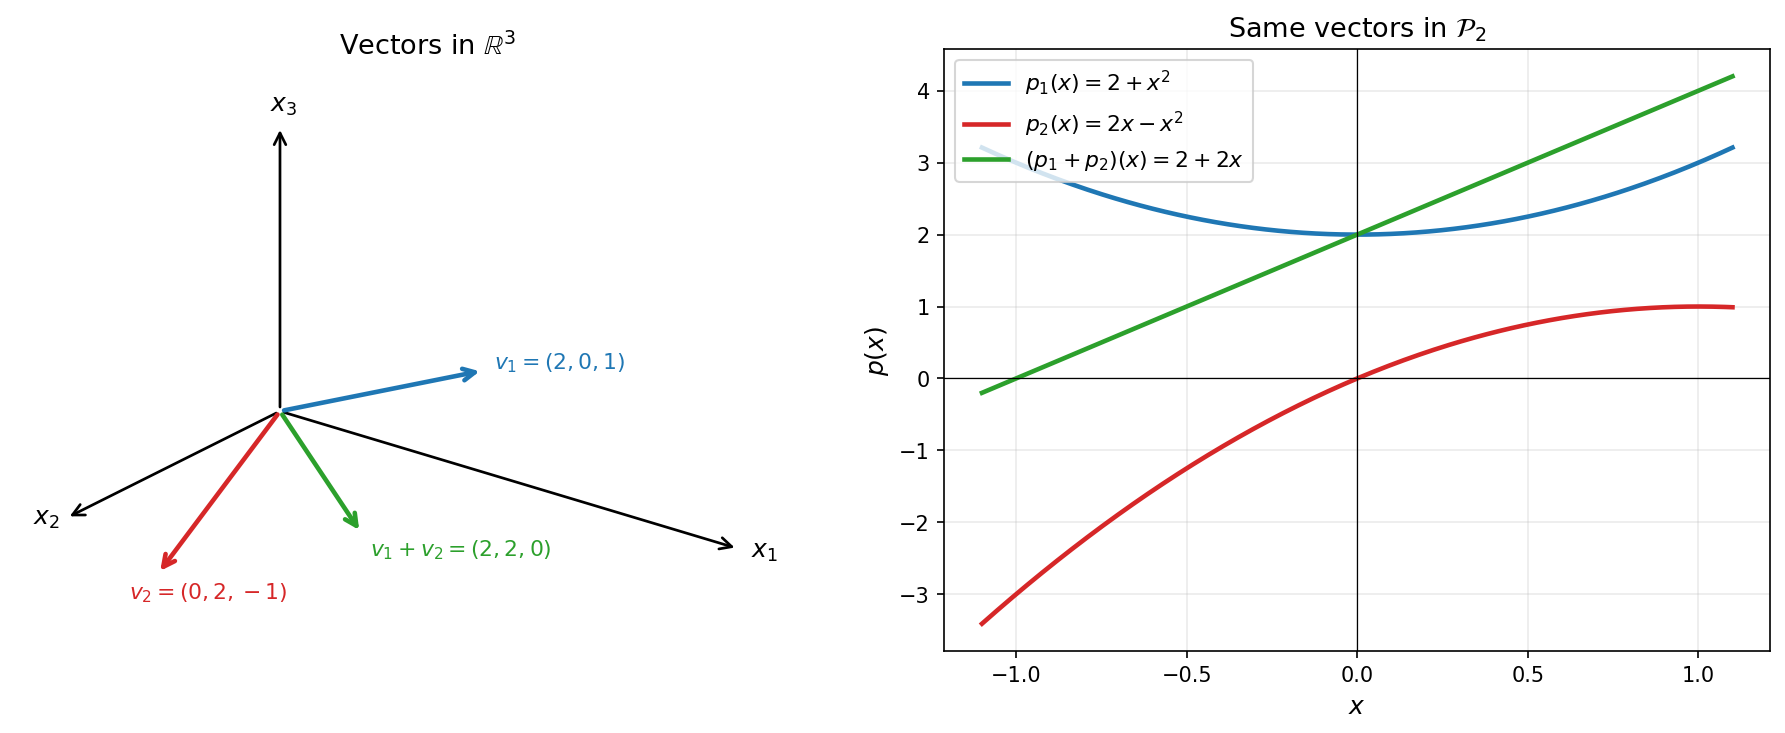
\includegraphics[width=\textwidth]{figures/fig01_vectors.png}
  \caption{The same abstract addition $v_1+v_2$ in two concrete spaces.
    \emph{Left:} arrows in $\mathbb{R}^3$ (oblique projection).
    \emph{Right:} polynomials in $\mathcal{P}_2$; the $x^2$ terms cancel,
    illustrating that the vector space axioms are the same regardless of
    what the objects ``look like''.}
\end{figure}

\begin{definition}
  A \emph{vector space} $V$ over a field $\mathbb{F}$ is a set of vectors
  equipped with two operations:
  \begin{itemize}
    \item addition $+: V\times V \to V$,
    \item scalar multiplication $\cdot\,: \mathbb{F}\times V \to V$,
  \end{itemize}
  satisfying the following eight axioms.  The quantifiers apply to
  \emph{all} $u,v,w\in V$ and \emph{all} $\lambda,\mu\in\mathbb{F}$ unless
  stated otherwise.
  \begin{enumerate}
    \item \textbf{Addition associativity:}
          $\forall\, u,v,w\in V:\quad (u+v)+w = u+(v+w)$.
    \item \textbf{Addition commutativity:}
          $\forall\, u,v\in V:\quad u+v = v+u$.
    \item \textbf{Additive identity:}
          $\exists\, 0\in V\;\forall\, v\in V:\quad v+0 = 0+v = v$.
    \item \textbf{Additive inverse:}
          $\forall\, v\in V\;\exists\, u\in V:\quad v+u = 0$.
          \hfill\textit{(we write $u=-v$)}
    \item \textbf{Scalar associativity:}
          $\forall\, \lambda,\mu\in\mathbb{F},\, v\in V:\quad
          (\lambda\mu)v = \lambda(\mu v)$.
    \item \textbf{Scalar distributivity:}
          $\forall\, \lambda,\mu\in\mathbb{F},\, v\in V:\quad
          (\lambda+\mu)v = \lambda v + \mu v$.
    \item \textbf{Vector distributivity:}
          $\forall\, \lambda\in\mathbb{F},\, u,v\in V:\quad
          \lambda(u+v) = \lambda u + \lambda v$.
    \item \textbf{Scalar identity:}
          $\exists\, 1\in\mathbb{F}\;\forall\, v\in V:\quad 1\cdot v = v$.
  \end{enumerate}
\end{definition}

\subsection*{Examples}

\begin{remark}[Examples are important]
  The axioms are necessary but dry.  Examples are where intuition lives.
  Every time you meet a new vector space, ask: what do addition and scalar
  multiplication \emph{mean} here?  What does the zero vector look like?
\end{remark}

\begin{example}\leavevmode
  \begin{enumerate}
    \item $V = \mathbb{F}^n$, $n\in\mathbb{N}$, $n\ge 1$.  This is the
      \emph{model example}: every finite-dimensional vector space is
      isomorphic to some $\mathbb{F}^n$, so understanding $\mathbb{F}^n$
      thoroughly means understanding all of finite-dimensional linear algebra.

    \item $V = \{0\}$ (the trivial vector space, with $0+0=0$ and
      $\lambda\cdot 0 = 0$).

    \item \textbf{Function spaces.}  Let $X$ be any set.  Then
      \[
        \mathbb{F}^X = \{f : X \to \mathbb{F}\}
      \]
      is a vector space under \emph{pointwise} operations:
      $(f+g)(x) = f(x)+g(x)$ and $(\lambda f)(x) = \lambda f(x)$.

      \textbf{Key sub-example.}  Take $X = [0,1]$ and $\mathbb{F}=\mathbb{R}$.
      Then $\mathbb{R}^{[0,1]}$ is the space of \emph{all} real-valued
      functions on $[0,1]$---it is \emph{infinite-dimensional}.  The
      trigonometric functions $\{1, \cos(n\pi x), \sin(n\pi x)\}_{n\ge 1}$
      form an orthogonal basis for the subspace of square-integrable
      functions (this is the starting point of \emph{Fourier analysis}).

    \item \textbf{RGB colors.}
      $c = (r,g,b)^T$ with $r,g,b\in\{0,1,\ldots,255\}$.

      \begin{exercise}
        Is the set of RGB color vectors a vector space over $\mathbb{R}$?
        If not, which axiom(s) fail?
      \end{exercise}

    \item \textbf{Polynomials of degree $\le n$.}
      \[
        \mathcal{P}_n = \{a_0 + a_1 x + \cdots + a_n x^n : a_i\in\mathbb{R}\}.
      \]
      Addition and scalar multiplication are defined coefficient-wise.
      The map
      \[
        \varphi: \mathcal{P}_n \longrightarrow \mathbb{R}^{n+1}, \qquad
        \varphi(a_0 + a_1 x + \cdots + a_n x^n) = (a_0, a_1, \ldots, a_n)^T
      \]
      is a bijection that respects both operations:
      $\varphi(\lambda p + \mu q) = \lambda\varphi(p) + \mu\varphi(q)$.
      Such a structure-preserving bijection is called an \emph{isomorphism}
      --- a ``sort of equality'' between seemingly different objects.
      So $\mathcal{P}_n \cong \mathbb{R}^{n+1}$ as vector spaces.

      \begin{exercise}
        Do polynomials of degree \emph{exactly} $n$ (i.e., $a_n \ne 0$)
        form a vector space?  Which axiom fails?
      \end{exercise}
  \end{enumerate}
\end{example}

\subsection*{Python: function spaces as vectors --- signals}
\begin{lstlisting}
import numpy as np
import matplotlib.pyplot as plt

# Discretise [0, 2pi] into N points: each signal is a vector in R^N
N = 512
t = np.linspace(0, 2 * np.pi, N)

# Two "vectors" in the function space R^[0,2pi]
f = np.sin(t)           # f(t) = sin(t)
g = np.cos(2 * t)       # g(t) = cos(2t)

# Vector addition and scalar multiplication are pointwise
h = f + 0.5 * g         # h = f + 0.5*g  (a new vector in the same space)

# Verify axiom 3 (zero vector): the zero function
zero = np.zeros(N)
print("f + zero == f:", np.allclose(f + zero, f))

# Verify axiom 4 (additive inverse): -f
print("f + (-f) == 0:", np.allclose(f + (-f), zero))

# Verify axiom 7 (distributivity): lambda*(f+g) == lambda*f + lambda*g
lam = 3.7
print("Distributivity:", np.allclose(lam * (f + g), lam * f + lam * g))

# Plot: three "vectors" in the function space
plt.figure(figsize=(8, 3))
plt.plot(t, f, label=r'$f = \sin t$')
plt.plot(t, g, label=r'$g = \cos 2t$')
plt.plot(t, h, label=r'$h = f + 0.5g$', linestyle='--')
plt.legend(); plt.title("Addition in the function space $\mathbb{R}^{[0,2\pi]}$")
plt.tight_layout(); plt.show()
\end{lstlisting}

\subsection*{Formal consequences of the axioms}

\begin{remark}[Why formal proofs?  Universality.]
  The propositions below are not hard.  The point is not the results
  themselves---they feel obvious.  The point is the \emph{technique}:
  every step must follow from the axioms alone, with no appeal to a
  specific example.  A proof that uses only the axioms works for
  \emph{every} vector space simultaneously: $\mathbb{R}^n$, function
  spaces, polynomial spaces, matrix spaces, spaces over $\mathbb{Z}_2$,
  spaces you have not yet imagined.  This is \emph{universality}.
  Abstraction is not the goal; universality is.
\end{remark}

\begin{proposition}[1.1.1 --- Uniqueness of zero]
  A vector space has a unique additive identity $0$.
\end{proposition}
\begin{proof}
  Suppose $0$ and $0'$ both satisfy axiom~3 (additive identity).  Then:
  \[
    0
    \stackrel{\text{ax.~3 on }0}{=} 0 + 0'
    \stackrel{\text{ax.~2}}{=} 0' + 0
    \stackrel{\text{ax.~3 on }0'}{=} 0'. \qedhere
  \]
\end{proof}

\begin{proposition}[1.1.2 --- Uniqueness of additive inverse]
  Every vector $v\in V$ has a unique additive inverse.
\end{proposition}
\begin{proof}
  Suppose $u$ and $w$ both satisfy axiom~4 for $v$: $v+u=0$ and $v+w=0$.
  Then:
  \[
    u
    \stackrel{\text{ax.~3}}{=} u + 0
    \stackrel{v+w=0}{=} u + (v + w)
    \stackrel{\text{ax.~1}}{=} (u + v) + w
    \stackrel{u+v=0}{=} 0 + w
    \stackrel{\text{ax.~2,~3}}{=} w. \qedhere
  \]
\end{proof}

\begin{proposition}[1.1.3]
  $\forall\, v\in V$:\; $0_{\mathbb{F}}\cdot v = 0_V$.
\end{proposition}
\begin{proof}
  In $\mathbb{F}$, $0_{\mathbb{F}} + 0_{\mathbb{F}} = 0_{\mathbb{F}}$, so:
  \[
    0_{\mathbb{F}}\cdot v
    = (0_{\mathbb{F}} + 0_{\mathbb{F}})\cdot v
    \stackrel{\text{ax.~6}}{=} 0_{\mathbb{F}}\cdot v + 0_{\mathbb{F}}\cdot v.
  \]
  Adding $-(0_{\mathbb{F}}\cdot v)$ (which exists by axiom~4) to both sides:
  $0_V = 0_{\mathbb{F}}\cdot v$.
\end{proof}

\begin{proposition}[1.1.4]
  $\forall\, \lambda\in\mathbb{F}$:\; $\lambda\cdot 0_V = 0_V$.
\end{proposition}
\begin{proof}
  By axiom~3, $0_V + 0_V = 0_V$, so:
  \[
    \lambda\cdot 0_V
    = \lambda\cdot(0_V + 0_V)
    \stackrel{\text{ax.~7}}{=} \lambda\cdot 0_V + \lambda\cdot 0_V.
  \]
  Adding $-(\lambda\cdot 0_V)$ to both sides: $0_V = \lambda\cdot 0_V$.
\end{proof}

\begin{proposition}[1.1.5]
  $\forall\, v\in V$:\; $(-1)\cdot v = -v$.
\end{proposition}
\begin{proof}
  Compute $v + (-1)\cdot v$:
  \[
    v + (-1)\cdot v
    \stackrel{\text{ax.~8}}{=} 1\cdot v + (-1)\cdot v
    \stackrel{\text{ax.~6}}{=} (1 + (-1))\cdot v
    = 0_{\mathbb{F}}\cdot v
    \stackrel{\text{Prop.~1.1.3}}{=} 0_V.
  \]
  So $(-1)\cdot v$ is an additive inverse of $v$.  By Prop.~1.1.2 the
  inverse is unique, hence $(-1)\cdot v = -v$.
\end{proof}

% ============================================================
\section{Subspaces}
% ============================================================

\begin{remark}[General philosophy]
  The ambient vector-space structure is trivial in the sense that the
  axioms are simple and few.  But within that shell, non-trivial structure
  emerges: subspaces, spans, bases, linear maps.  The game is always the
  same --- start from the universal axioms, derive consequences that hold
  for \emph{every} vector space at once.
\end{remark}

\noindent\textit{Notation.} $V$ denotes a vector space over $\mathbb{F}$
(take $\mathbb{F}=\mathbb{R}$ whenever a specific field is not mentioned).

\begin{definition}[\S1.2]
  A subset $U\subseteq V$ is a \emph{subspace} (written $U\le V$) if:
  \begin{enumerate}
    \item $0\in U$,
    \item $U$ is closed under addition:
          $\forall\, u,v\in U:\; u+v\in U$,
    \item $U$ is closed under scalar multiplication:
          $\forall\, \lambda\in\mathbb{F},\, u\in U:\; \lambda u\in U$.
  \end{enumerate}
\end{definition}

\begin{figure}[h!]
  \centering
  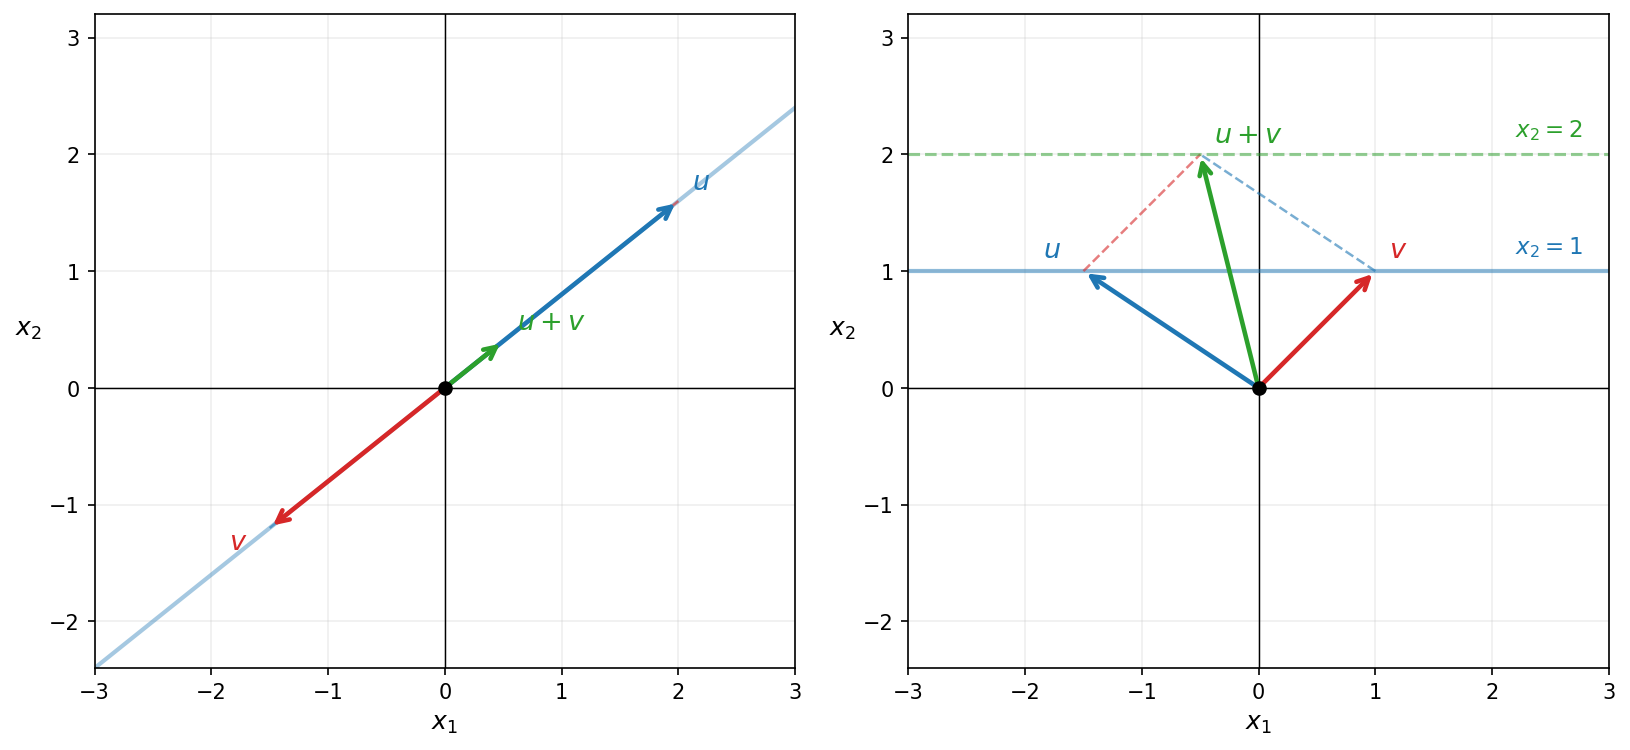
\includegraphics[width=\textwidth]{figures/fig02_subspace.png}
  \caption{Subspace vs.\ affine subspace in $\mathbb{R}^2$.
    \emph{Left:} the line through the origin is a subspace --- vectors $u$,
    $v$, and their sum $u+v$ all lie on it.
    \emph{Right:} the line $x_2=1$ is not a subspace --- $u+v$ escapes to
    $x_2=2$, violating closure under addition (and $0\notin U$).}
\end{figure}

\begin{proposition}[Subspace test --- one condition]
  A nonempty subset $U\subseteq V$ is a subspace if and only if
  \[
    \forall\, u,v\in U,\; \forall\,\lambda\in\mathbb{F}:\quad \lambda u + v\in U.
  \]
\end{proposition}
\begin{proof}
  ($\Rightarrow$) If $U$ is a subspace, closure under scalar multiplication
  gives $\lambda u\in U$, and then closure under addition gives
  $\lambda u + v\in U$.

  ($\Leftarrow$) Set $\lambda=0$: $0\cdot u + v = v\in U$, so $U$ is closed
  under addition.  Set $v=0$: $\lambda u + 0 = \lambda u\in U$, so $U$ is
  closed under scalar multiplication.  For the zero vector, pick any $u\in U$
  (nonempty) and set $\lambda=0$, $v=0$: $0\in U$.
\end{proof}

\begin{example}[Trivial subspaces]
  Every vector space $V$ has exactly two \emph{trivial subspaces}: $\{0\}$
  and $V$ itself.
  \begin{itemize}
    \item $\{0\}$ satisfies the definition for the dumbest possible reason:
          it contains only the zero vector, so every condition is vacuously
          or trivially met.
    \item $V$ satisfies the definition because it is already a vector space,
          so closure holds by the axioms.
  \end{itemize}
  Any subspace strictly between $\{0\}$ and $V$ is \emph{non-trivial}, and
  these are the interesting ones.
\end{example}

\begin{example}[Non-example: affine shifts are not subspaces]
  Let $U\le V$ be a subspace and $c\in V$ with $c\ne 0$.  The
  \emph{affine set}
  \[
    U + c = \{u + c : u\in U\}
  \]
  is \emph{not} a subspace: it fails condition~1, since $0 = u+c$ would
  require $u = -c\in U$, but then $c = -u\in U$ (as $U$ is closed under
  scalar mult with $\lambda=-1$), contradicting $c\notin U$ if $c\ne 0$
  and $0\notin U+c$ in general.

  \textbf{Concrete instance.}  In $\mathbb{R}^2$, the line
  $\ell = \{(x,1) : x\in\mathbb{R}\}$ is an affine shift of the $x$-axis
  (a subspace) by the vector $(0,1)^T$.  It does not pass through the
  origin, so it is not a subspace.
\end{example}

\begin{example}[$\mathcal{P}_1 \le \mathcal{P}_3$]
  Let $V = \mathcal{P}_3$ and $U = \{mx + b : m,b\in\mathbb{R}\}$
  (polynomials of degree $\le 1$).  We verify the three conditions:
  \begin{enumerate}
    \item $0\in U$: take $m=b=0$, giving the zero polynomial. \checkmark
    \item Closed under addition: $(m_1 x+b_1)+(m_2 x+b_2) = (m_1+m_2)x+(b_1+b_2)\in U$. \checkmark
    \item Closed under scalar mult: $\lambda(mx+b) = (\lambda m)x+(\lambda b)\in U$. \checkmark
  \end{enumerate}
  Hence $U = \mathcal{P}_1 \le \mathcal{P}_3$.
\end{example}

\begin{example}[Homogeneous vs.\ inhomogeneous linear constraints]
  Let $V = \mathbb{R}^4$ and $b\in\mathbb{R}$ a fixed constant.  Consider
  \[
    U_b = \{(x_1,x_2,x_3,t)^T\in\mathbb{R}^4 : x_3 = 5x_1 + b\}.
  \]
  \textbf{Claim:} $U_b$ is a subspace if and only if $b = 0$.
  \begin{proof}
    ($b=0$) The constraint $x_3 = 5x_1$ is \emph{homogeneous} (passes
    through the origin).  Check: $0\in U_0$ since $0=5\cdot 0$.  If
    $u,v\in U_0$ then $(u+v)_3 = u_3+v_3 = 5u_1+5v_1 = 5(u+v)_1$, so
    $u+v\in U_0$.  Similarly $(\lambda u)_3 = \lambda u_3 = 5\lambda u_1$,
    so $\lambda u\in U_0$.  Hence $U_0\le V$.

    ($b\ne 0$) The zero vector requires $0 = 5\cdot 0 + b = b \ne 0$,
    a contradiction.  So $0\notin U_b$, and condition~1 fails.
  \end{proof}
  \textbf{Moral:} a linear constraint defines a subspace iff it is
  \emph{homogeneous} (constant term zero).  Inhomogeneous constraints give
  affine subsets, not subspaces.
\end{example}

\subsection*{Sum and direct sum of subspaces}

\begin{definition}
  Let $V_1, V_2, \ldots, V_m \le V$ be subspaces.  Their \emph{sum} is
  \[
    V_1 + V_2 + \cdots + V_m
    = \{v_1 + v_2 + \cdots + v_m : v_i\in V_i,\; i=1,\ldots,m\}.
  \]
\end{definition}

\begin{exercise}
  What is the sum of
  \[
    U = \{(x, x, y, y)^T\in\mathbb{R}^4 : x,y\in\mathbb{R}\}
    \quad\text{and}\quad
    W = \{(x, x, x, y)^T\in\mathbb{R}^4 : x,y\in\mathbb{R}\}?
  \]
\end{exercise}

\begin{proposition}[1.2.1]
  Let $V_1,\ldots,V_m\le V$ be subspaces.  Then $V_1+\cdots+V_m$ is the
  \emph{smallest} subspace of $V$ containing each $V_i$.
\end{proposition}
\begin{proof}
  \textit{It is a subspace.}
  $0 = 0+\cdots+0\in V_1+\cdots+V_m$ (taking $v_i=0\in V_i$).
  If $w = \sum v_i$ and $w' = \sum v_i'$ are two elements, then
  $w+w' = \sum(v_i+v_i')$ with $v_i+v_i'\in V_i$, so $w+w'$ is in the sum.
  Similarly $\lambda w = \sum(\lambda v_i)$ with $\lambda v_i\in V_i$.

  \textit{It contains each $V_i$.}
  Given $v\in V_i$, write $v = 0+\cdots+0+v+0+\cdots+0$
  ($v$ in position $i$, zeros elsewhere); this is in $V_1+\cdots+V_m$.

  \textit{It is the smallest.}
  Let $W\le V$ be any subspace containing each $V_i$.  Any element
  $\sum v_i$ (with $v_i\in V_i\subseteq W$) belongs to $W$ by closure under
  addition, so $V_1+\cdots+V_m\subseteq W$.
\end{proof}

\begin{definition}[Direct sum]
  The sum $W = V_1+\cdots+V_m$ is a \emph{direct sum}, written
  $W = V_1\oplus\cdots\oplus V_m$, if every $w\in W$ can be written in
  \emph{exactly one way} as $w = v_1+\cdots+v_m$ with $v_i\in V_i$.
\end{definition}

\begin{proposition}[Equivalent characterizations of direct sum]
  The following are equivalent:
  \begin{enumerate}[label=(\roman*)]
    \item $W = V_1\oplus\cdots\oplus V_m$.
    \item $W = V_1+\cdots+V_m$ and $v_1+\cdots+v_m = 0$ with $v_i\in V_i$
          implies $v_i = 0$ for all $i$.
    \item $W = V_1+\cdots+V_m$ and
          $V_i \cap \displaystyle\sum_{j\ne i} V_j = \{0\}$ for all $i$.
  \end{enumerate}
  \textbf{Special case $m=2$:} $W = V_1\oplus V_2$ iff $W = V_1+V_2$ and
  $V_1\cap V_2 = \{0\}$.
\end{proposition}
\begin{proof}
  (i)$\Rightarrow$(ii): If the representation is unique and $v_1+\cdots+v_m=0$,
  then $0+\cdots+0=0$ is another representation, so by uniqueness each $v_i=0$.

  (ii)$\Rightarrow$(iii): Suppose $u\in V_i\cap\sum_{j\ne i}V_j$.  Then
  $u = \sum_{j\ne i}v_j$ for some $v_j\in V_j$, so
  $v_1+\cdots+(-u)+\cdots+v_m = 0$ (with $-u$ in position $i$).
  By~(ii) each term is $0$, so $u=0$.

  (iii)$\Rightarrow$(i): If $\sum v_i = \sum v_i'$ then
  $\sum(v_i-v_i')=0$, so $v_i-v_i' = -\sum_{j\ne i}(v_j-v_j')
  \in V_i\cap\sum_{j\ne i}V_j = \{0\}$, giving $v_i=v_i'$.
\end{proof}

\subsection*{Python: direct sum decomposition and uniqueness}
\begin{lstlisting}
import numpy as np

# R^4 = V1 + V2 where:
#   V1 = span{e1, e2}  (first two coords free, last two zero)
#   V2 = span{e3, e4}  (first two zero, last two coords free)
# This is a direct sum: V1 \cap V2 = {0}.

def project_V1(v): return np.array([v[0], v[1], 0, 0])
def project_V2(v): return np.array([0, 0, v[2], v[3]])

v = np.array([3., -1., 2., 5.])
v1 = project_V1(v)
v2 = project_V2(v)

print("v  =", v)
print("v1 =", v1, " (component in V1)")
print("v2 =", v2, " (component in V2)")
print("v1 + v2 == v:", np.allclose(v1 + v2, v))   # True: decomposition works
print("V1 \cap V2 = {0}:", np.allclose(project_V1(v2), 0) and
                         np.allclose(project_V2(v1), 0))

# Now a NON-direct sum: V3 = span{e1+e2}, V4 = span{e1}
# V3 + V4 = span{e1, e2} but V3 \cap V4 \neq {0}
V3_basis = np.array([1., 1.])   # in R^2 for simplicity
V4_basis = np.array([1., 0.])
w = np.array([2., 1.])

# Two different decompositions of w in V3 + V4:
# w = 1*(1,1) + 1*(1,0)  ->  coeffs (1, 1)
# w = 0*(1,1) + 2*(1,0)  -> not valid since 0*(1,1) is in V3 but
# Actually let's solve: w = a*(1,1) + b*(1,0)
# => a+b=2, a=1 => unique. But try a degenerate case:
V3b = np.array([1., 1.])
V4b = np.array([2., 2.])  # parallel to V3b -> NOT direct sum
A = np.column_stack([V3b, V4b])
print("\nParallel subspaces (not direct sum):")
print("Rank of [V3, V4]:", np.linalg.matrix_rank(A),
      " (should be 1, not 2 -> not direct sum)")
\end{lstlisting}

\subsection*{Python: numerically testing the subspace conditions}
\begin{lstlisting}
import numpy as np

rng = np.random.default_rng(42)

def is_subspace_numeric(sample_fn, n_trials=2000, tol=1e-10):
    """
    Numerically test whether a set U (described by sample_fn) looks
    like a subspace of R^n.  sample_fn() should return a random element of U.
    Tests: (1) zero in U, (2) closed under addition, (3) closed under scaling.
    """
    # Condition 1: zero vector
    zero = np.zeros_like(sample_fn())
    # We check it by seeing if 0*u is in U (i.e. looks like a sample)
    # Here we just verify sample_fn produces things near the zero-pattern

    failures = 0
    for _ in range(n_trials):
        u = sample_fn()
        v = sample_fn()
        lam = rng.uniform(-5, 5)

        # Condition 2: u + v should satisfy the same constraint as U
        # Condition 3: lam * u should satisfy the same constraint
        # We test these for two specific subspaces below.
        _ = lam * u + v   # just compute; constraint checked per-example

    return failures == 0

# Subspace: U = {(x1, x2, x3) : x3 = 5*x1}  (homogeneous -> subspace)
def sample_U():
    x1, x2 = rng.standard_normal(2)
    return np.array([x1, x2, 5 * x1])

def in_U(v, tol=1e-9):
    return abs(v[2] - 5 * v[0]) < tol

n_trials = 2000
u_fails = sum(
    not in_U(rng.uniform(-5,5) * sample_U() + sample_U())
    for _ in range(n_trials)
)
print(f"U (homogeneous): {u_fails}/{n_trials} failures  -> subspace: {u_fails==0}")

# Non-subspace: W = {(x1, x2, x3) : x3 = 5*x1 + 1}  (inhomogeneous)
def sample_W():
    x1, x2 = rng.standard_normal(2)
    return np.array([x1, x2, 5 * x1 + 1])

def in_W(v, tol=1e-9):
    return abs(v[2] - 5 * v[0] - 1) < tol

w_fails = sum(
    not in_W(rng.uniform(-5,5) * sample_W() + sample_W())
    for _ in range(n_trials)
)
print(f"W (inhomogeneous): {w_fails}/{n_trials} failures -> subspace: {w_fails==0}")
\end{lstlisting}

% ============================================================
\section{Span and Linear Independence}
% ============================================================

\begin{remark}[Theory meets computation]
  The abstract theory tells us \emph{what} subspaces are.  To actually
  \emph{find} them --- compute bases, check independence, determine whether
  a vector lies in a span --- we need row reduction and matrix algorithms.
  From here onward, theory and computation go hand in hand.
\end{remark}

\subsection*{\S1.3 Linear combinations and span}

\begin{definition}
  A \emph{linear combination} of vectors $v_1,\ldots,v_p\in V$ is any
  expression $\sum_{k=1}^p \lambda_k v_k$ with $\lambda_k\in\mathbb{F}$.
  It is \emph{trivial} if all $\lambda_k = 0$.

  The \emph{span} of $\{v_1,\ldots,v_p\}$ is the set of all their linear
  combinations:
  \[
    \operatorname{span}\{v_1,\ldots,v_p\}
    = \langle v_1,\ldots,v_p\rangle
    = \left\{\sum_{k=1}^p \lambda_k v_k : \lambda_k\in\mathbb{F}\right\}.
  \]
  A set $\{v_1,\ldots,v_p\}$ is a \emph{generating} (or \emph{spanning})
  \emph{system} for $V$ if $\operatorname{span}\{v_1,\ldots,v_p\} = V$.
\end{definition}

\begin{proposition}[Span is the smallest containing subspace]
  $\operatorname{span}\{v_1,\ldots,v_p\}$ is a subspace of $V$, and it is
  the \emph{smallest} subspace containing all of $v_1,\ldots,v_p$.
\end{proposition}
\begin{proof}
  \textit{It is a subspace.}
  $0 = \sum_k 0\cdot v_k \in \operatorname{span}$.
  If $u = \sum_k \lambda_k v_k$ and $w = \sum_k \mu_k v_k$, then
  $u + w = \sum_k(\lambda_k+\mu_k)v_k \in \operatorname{span}$ and
  $\alpha u = \sum_k (\alpha\lambda_k)v_k \in \operatorname{span}$.

  \textit{It contains each $v_i$.}
  Take $\lambda_i = 1$ and $\lambda_k = 0$ for $k\ne i$.

  \textit{It is the smallest.}
  Let $W\le V$ contain each $v_i$.  Any linear combination
  $\sum_k \lambda_k v_k$ belongs to $W$ by closure, so
  $\operatorname{span}\{v_1,\ldots,v_p\}\subseteq W$.
\end{proof}

\begin{example}[Span in $\mathbb{R}^2$]
  \leavevmode
  \begin{itemize}
    \item $\operatorname{span}\{(1,0)^T,(0,1)^T\} = \mathbb{R}^2$:
      any $(a,b)^T = a(1,0)^T + b(0,1)^T$. \quad
      These two vectors are linearly independent.
    \item $\operatorname{span}\{(1,1)^T,(2,2)^T\} = \{(t,t)^T:t\in\mathbb{R}\}
      \subsetneq \mathbb{R}^2$:
      both vectors point in the same direction, so their span is a line.
      These two vectors are linearly \emph{dependent}: $(2,2)^T = 2(1,1)^T$.
  \end{itemize}
  \textbf{Lesson:} whether a set spans depends on linear independence, not
  just on the number of vectors.
\end{example}

\begin{figure}[h!]
  \centering
  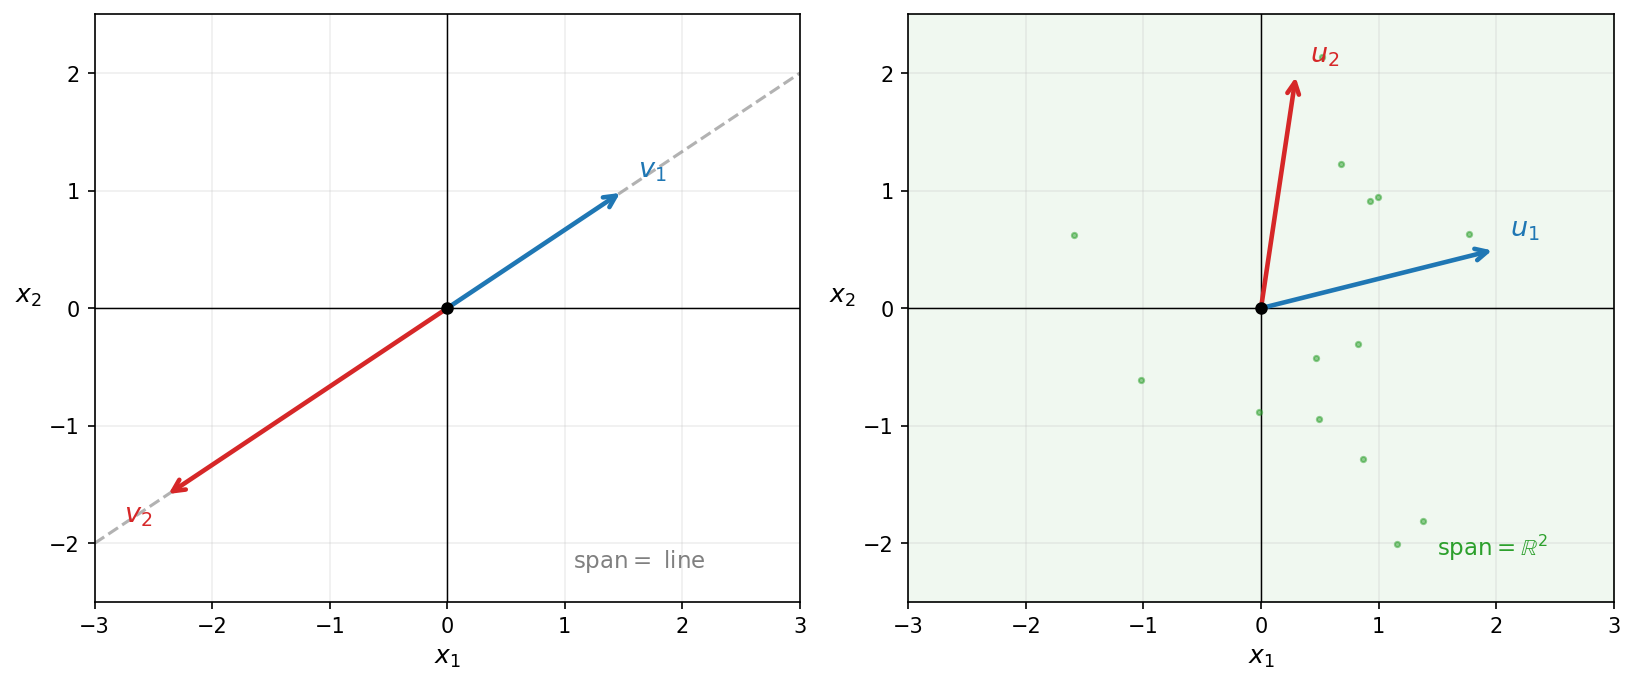
\includegraphics[width=\textwidth]{figures/fig03_span.png}
  \caption{Span in $\mathbb{R}^2$.
    \emph{Left:} collinear $v_1,v_2$ --- span is a line.
    \emph{Right:} linearly independent $u_1,u_2$ --- span fills $\mathbb{R}^2$
    (shaded, with sample points).}
\end{figure}

\subsection*{Python: checking span via rank}
\begin{lstlisting}
import numpy as np

# Do v1, v2, v3 span R^3?
V = np.array([[1, 0, 1],
              [0, 1, 1],
              [0, 0, 0]], float)   # columns are the vectors
rank = np.linalg.matrix_rank(V)
n = V.shape[0]
print("rank =", rank, "  spans R^3:", rank == n)
# rank=2, so they do NOT span R^3

# Does a target vector b lie in the span?
b = np.array([1, 1, 0], float)
# Augment and check if rank increases
aug = np.column_stack([V, b])
print("b in span:", np.linalg.matrix_rank(aug) == rank)
\end{lstlisting}

\begin{definition}
  A set of vectors $\{v_1,\ldots,v_p\}$ is \emph{linearly dependent} if
  there exist scalars $\lambda_1,\ldots,\lambda_p$, \emph{not all zero},
  such that $\sum_{k=1}^p \lambda_k v_k = 0$.

  The set is \emph{linearly independent} if the only solution to
  $\sum_{k=1}^p \lambda_k v_k = 0$ is the trivial one ($\lambda_k=0$ for
  all $k$).
\end{definition}

\begin{proposition}[Linear dependence $\iff$ one vector is redundant]
  A set $\{v_1,\ldots,v_p\}\subset V$ is linearly dependent if and only if
  there exists an index $k\in\{1,\ldots,p\}$ such that
  \[
    v_k = \sum_{\substack{j=1\\j\ne k}}^p \beta_j\, v_j.
  \]
\end{proposition}
\begin{proof}
  ($\Rightarrow$) Suppose $\sum_{i=1}^p \lambda_i v_i = 0$ with some
  $\lambda_k\ne 0$.  Then
  \[
    \lambda_k v_k = -\sum_{j\ne k}\lambda_j v_j
    \implies
    v_k = \sum_{j\ne k}\left(-\frac{\lambda_j}{\lambda_k}\right)v_j.
  \]

  ($\Leftarrow$) If $v_k = \sum_{j\ne k}\beta_j v_j$, then
  \[
    \sum_{j\ne k}\beta_j v_j + (-1)\cdot v_k = 0,
  \]
  which is a nontrivial relation (the coefficient of $v_k$ is $-1\ne 0$).
\end{proof}

\begin{example}
  \leavevmode
  \begin{itemize}
    \item In $\mathcal{P}_n$: the monomials $\{1, x, x^2, \ldots, x^n\}$
      are linearly independent, since a polynomial identically equal to zero
      has all coefficients zero.
    \item In $\mathbb{R}^3$: the standard basis vectors
      $\{e_1,e_2,e_3\}$ are independent; $\{(1,0,0)^T,(2,0,0)^T\}$ are
      dependent since $(2,0,0)^T = 2(1,0,0)^T$.
  \end{itemize}
\end{example}

\begin{example}[Uniqueness of representation]
  If $V = \langle v_1,\ldots,v_p\rangle$ and $\{v_1,\ldots,v_p\}$ is
  linearly independent, then every $x\in V$ has a \emph{unique}
  representation $x = \sum_k \lambda_k v_k$.
  \begin{proof}
    If $\sum_k \lambda_k v_k = x = \sum_k \mu_k v_k$, then
    $\sum_k(\lambda_k-\mu_k)v_k = 0$.  Linear independence forces
    $\lambda_k = \mu_k$ for all $k$.
  \end{proof}
  This uniqueness is exactly why we care about independent spanning sets
  (bases): they give a \emph{coordinate system}.
\end{example}

% ============================================================
\section{Bases and Dimension}
% ============================================================

\begin{definition}[Basis via direct sum]
  A set $\{v_1,\ldots,v_n\}\subset V$ is a \emph{basis} of $V$ if
  \[
    V = \langle v_1\rangle \oplus \langle v_2\rangle \oplus \cdots
        \oplus \langle v_n\rangle,
  \]
  where $\langle v_i\rangle = \{\lambda v_i : \lambda\in\mathbb{F}\}$ is the
  one-dimensional subspace spanned by $v_i$.
\end{definition}

\begin{remark}[Coordinates]
  The direct sum condition says exactly that every $v\in V$ has a
  \emph{unique} representation
  \[
    v = \lambda_1 v_1 + \lambda_2 v_2 + \cdots + \lambda_n v_n,
    \qquad \lambda_i\in\mathbb{F}.
  \]
  The map
  \[
    \varphi_B : V \longrightarrow \mathbb{F}^n,
    \qquad
    v \longmapsto (\lambda_1,\ldots,\lambda_n)^T
  \]
  is an isomorphism --- it identifies $V$ with $\mathbb{F}^n$.  Different
  bases give different isomorphisms, i.e.\ different coordinate systems.
  This is why all $n$-dimensional vector spaces over $\mathbb{F}$ are
  ``the same'': they are all isomorphic to $\mathbb{F}^n$.
\end{remark}

\begin{proposition}[Basis characterization --- two definitions agree]
  The following are equivalent for a set $\{v_1,\ldots,v_n\}\subset V$:
  \begin{enumerate}[label=(\roman*)]
    \item $V = \langle v_1\rangle\oplus\cdots\oplus\langle v_n\rangle$
          (basis via direct sum).
    \item $\{v_1,\ldots,v_n\}$ is a linearly independent spanning set.
    \item $\{v_1,\ldots,v_n\}$ is a \emph{minimal} spanning set (removing
          any one vector destroys span).
    \item $\{v_1,\ldots,v_n\}$ is a \emph{maximal} linearly independent
          set (adding any vector creates dependence).
  \end{enumerate}
\end{proposition}
\begin{proof}
  (i)$\iff$(ii): The direct sum $V=\bigoplus_i\langle v_i\rangle$ means every
  $v\in V$ is uniquely $\sum_i\lambda_i v_i$.  This is spanning.  Uniqueness
  with $v=0$ gives $\sum_i\lambda_i v_i=0\Rightarrow\lambda_i=0$ for all $i$,
  which is linear independence.  Conversely, independence + spanning gives
  uniqueness of representation, which is the direct sum condition.

  (ii)$\Rightarrow$(iii): If some $v_k$ can be removed and the rest still
  span, then $v_k\in\operatorname{span}\{v_j:j\ne k\}$, contradicting independence.

  (iii)$\Rightarrow$(ii): A minimal spanning set must be independent (otherwise
  remove a redundant vector by the previous proposition and still span).

  (ii)$\Rightarrow$(iv): Adding any $w\in V$ to the set: write $w=\sum\lambda_i v_i$
  (by spanning); then $w - \sum\lambda_i v_i = 0$ is a nontrivial relation.

  (iv)$\Rightarrow$(ii): Maximality forces every $w\in V$ to be in the span
  (otherwise $\{v_1,\ldots,v_n,w\}$ would be independent, contradicting maximality).
\end{proof}

\subsection*{Python: coordinates in a basis}
\begin{lstlisting}
import numpy as np

# Basis vectors as columns of B
B = np.array([[1, 1, 0],
              [0, 1, 1],
              [1, 0, 1]], float)

v = np.array([3, 2, 1], float)

# Coordinates of v in basis B: solve B @ coords = v
coords = np.linalg.solve(B, v)
print("Coordinates:", coords)

# Verify: reconstruct v from coordinates
print("Reconstructed:", B @ coords)    # should equal v

# Different basis => different coordinates for the same vector
B2 = np.eye(3)                         # standard basis
coords2 = np.linalg.solve(B2, v)
print("Standard coords:", coords2)     # just v itself
\end{lstlisting}

\subsection*{Python: differentiation as a matrix --- and nilpotency}
\begin{lstlisting}
import numpy as np

# Build the differentiation matrix D for P_n in the monomial basis
# {1, x, x^2, ..., x^n}  (represented as coefficient vectors in R^{n+1})
# D(x^k) = k * x^{k-1},  D(1) = 0

def diff_matrix(n):
    """(n+1) x (n+1) matrix of D: P_n -> P_n in monomial basis."""
    D = np.zeros((n + 1, n + 1))
    for k in range(1, n + 1):
        D[k - 1, k] = k   # coefficient of x^{k-1} in D(x^k) is k
    return D

D = diff_matrix(5)
print("D =\n", D.astype(int))

# Verify: D * [0,0,1,0,0,0]^T = coeff vector of D(x^2) = 2x = [0,2,0,0,0,0]
x2_coeffs = np.array([0, 0, 1, 0, 0, 0], float)
print("D(x^2) coeffs:", D @ x2_coeffs)   # should be [0, 2, 0, 0, 0, 0]

# D is NILPOTENT: D^{n+1} = 0
print("D^6 = 0:", np.allclose(np.linalg.matrix_power(D, 6), 0))

# Show the staircase of powers
for k in range(1, 7):
    Dk = np.linalg.matrix_power(D, k)
    rank = np.linalg.matrix_rank(Dk)
    print(f"  rank(D^{k}) = {rank}")   # 5, 4, 3, 2, 1, 0

# Integrate back: J = right inverse of D.  J(x^k) = x^{k+1}/(k+1)
def antideriv_matrix(n):
    """(n+2) x (n+1) matrix of J: P_n -> P_{n+1}."""
    J = np.zeros((n + 2, n + 1))
    for k in range(n + 1):
        J[k + 1, k] = 1.0 / (k + 1)
    return J

J = antideriv_matrix(5)
D6 = diff_matrix(6)   # D acting on P_6 (to compose with J: P_5->P_6)
print("D o J = I:", np.allclose(D6 @ J, np.eye(6)))   # True: FTC
\end{lstlisting}

\begin{remark}[A basis makes everything computable]
  Once a basis $\{v_1,\ldots,v_n\}$ of $V$ is fixed, the coordinate
  isomorphism $\varphi_B: V\to\mathbb{F}^n$ turns every abstract vector
  into a concrete column of numbers, and every linear map into a matrix.
  The choice of basis is the choice of coordinate system; the mathematics
  is independent of that choice, but the computations depend on it.
  A good basis (e.g.\ an orthonormal one; see \S3) makes computations fast and
  numerically stable.
\end{remark}

\subsection*{\S1.9 Matrices --- a practical bridge}

\begin{example}[Digital images as matrices]
  A \textbf{color image} $N = (R,G,B)$ is stored as three separate
  $m\times n$ arrays of pixel intensities, one per channel.  Each entry
  is an integer in $\{0,\ldots,255\}$.

  A \textbf{grayscale image} collapses to a single $m\times n$ array:
  \[
    A \in \{0,1,\ldots,255\}^{m\times n} \subset \mathbb{R}^{m\times n}.
  \]
  A typical photograph might have $m=3024$, $n=4032$, giving over
  $12$ million entries per channel --- expensive to store or transmit raw.

  \textbf{Key observation.} Natural images are not random matrices: rows
  and columns are highly correlated (nearby pixels look similar).  This
  means the matrix $A$ is \emph{approximately low-rank}: most of its
  information lives in a small number of directions.

  \textbf{Forward pointer.} The Singular Value Decomposition (SVD) gives
  the \emph{best} low-rank approximation to any matrix:
  \[
    A \approx A_k = \sum_{i=1}^k \sigma_i u_i v_i^T, \qquad k \ll \min(m,n).
  \]
  JPEG compression, Netflix recommendations, and PCA in genomics all
  exploit this idea.  We will prove the optimality of this approximation
  (Eckart--Young theorem) later in the course.
\end{example}

\subsection*{Python: images as matrices}
\begin{lstlisting}
import numpy as np
import matplotlib.pyplot as plt

# Create a synthetic grayscale "image" (or load a real one)
rng = np.random.default_rng(0)
m, n = 64, 64
# Low-rank signal + noise: true rank is 3
U = rng.standard_normal((m, 3))
V = rng.standard_normal((n, 3))
A = U @ V.T + 0.5 * rng.standard_normal((m, n))

# SVD
u, s, vt = np.linalg.svd(A, full_matrices=False)
print("Singular values (first 6):", np.round(s[:6], 2))

# Rank-k approximations and their errors
for k in [1, 3, 10]:
    Ak = u[:, :k] @ np.diag(s[:k]) @ vt[:k, :]
    err = np.linalg.norm(A - Ak, 'fro') / np.linalg.norm(A, 'fro')
    print(f"  k={k:2d}  relative Frobenius error: {err:.3f}")
\end{lstlisting}

\begin{definition}
  A \emph{matrix} over $\mathbb{F}$ is a rectangular array with $m$ rows and
  $n$ columns, with entries in $\mathbb{F}$:
  \[
    A = (a_{ij})_{\substack{i=1,\ldots,m\\j=1,\ldots,n}} \in \mathbb{F}^{m\times n}.
  \]
  The $(i,j)$-entry of $A$ is $(A)_{ij} = a_{ij}$.  The $j$-th column of
  $A$ is the vector $a_j = (a_{1j},\ldots,a_{mj})^T\in\mathbb{F}^m$.

  \textbf{Operations} (defined entry-wise):
  \begin{itemize}
    \item Addition: $(A+B)_{ij} = a_{ij} + b_{ij}$.
    \item Scalar multiplication: $(\lambda A)_{ij} = \lambda\, a_{ij}$.
  \end{itemize}
\end{definition}

\begin{proposition}
  $\mathbb{F}^{m\times n}$ is a vector space over $\mathbb{F}$ of dimension $mn$.
\end{proposition}
\begin{proof}
  \textit{Vector space.}  Define the \emph{vec} operation: stack the columns
  of $A$ into a single vector,
  \[
    \operatorname{vec}(A) = (a_{11},\ldots,a_{m1},\, a_{12},\ldots,a_{m2},\,
    \ldots,\, a_{1n},\ldots,a_{mn})^T \in \mathbb{F}^{mn}.
  \]
  Then $\operatorname{vec}$ is a bijection that respects addition and scalar
  multiplication, so $\mathbb{F}^{m\times n}\cong\mathbb{F}^{mn}$ as vector
  spaces.  All 8 axioms are inherited entry-wise from $\mathbb{F}$.

  \textit{Dimension and basis.}  Define the \emph{standard matrix units}
  $E_{ij}\in\mathbb{F}^{m\times n}$ as the matrix with $1$ in position
  $(i,j)$ and $0$ elsewhere.  Every matrix decomposes uniquely as
  \[
    A = \sum_{i=1}^m \sum_{j=1}^n a_{ij}\, E_{ij},
  \]
  so $\{E_{ij}\}$ is a basis of $\mathbb{F}^{m\times n}$ with $mn$ elements.
  Hence $\dim\mathbb{F}^{m\times n} = mn$.
\end{proof}

\begin{definition}[Transpose]
  The \emph{transpose} of $A\in\mathbb{F}^{m\times n}$ is
  $A^T\in\mathbb{F}^{n\times m}$ defined by $(A^T)_{ij} = a_{ji}$.
  Equivalently, the columns of $A^T$ are the rows of $A$, and vice versa.
\end{definition}

\begin{proposition}[Transpose properties]
  \leavevmode
  \begin{enumerate}[label=(\alph*)]
    \item $(A^T)^T = A$.
    \item $(\lambda A + \mu B)^T = \lambda A^T + \mu B^T$ (linearity).
    \item $(AB)^T = B^T A^T$ \quad (order reverses).
  \end{enumerate}
\end{proposition}
\begin{proof}
  (a) $((A^T)^T)_{ij} = (A^T)_{ji} = a_{ij}$.

  (b) Entry-wise: $(\lambda A+\mu B)^T_{ij} = \lambda a_{ji}+\mu b_{ji}
  = (\lambda A^T+\mu B^T)_{ij}$.

  (c) $((AB)^T)_{ij} = (AB)_{ji} = \sum_k a_{jk}b_{ki}
  = \sum_k (B^T)_{ik}(A^T)_{kj} = (B^TA^T)_{ij}$.
\end{proof}

\begin{remark}
  Since the column space of $A^T$ is the row space of $A$, the four
  fundamental subspaces of $A$ come in two transpose-related pairs:
  $\operatorname{col}(A)\perp\ker(A^T)$ and
  $\operatorname{row}(A)\perp\ker(A)$.
\end{remark}

\begin{definition}[Matrix-vector product]
  For $A\in\mathbb{F}^{m\times n}$ and $x\in\mathbb{F}^n$, the
  \emph{matrix-vector product} $Ax\in\mathbb{F}^m$ is
  \[
    Ax = \sum_{j=1}^n x_j\, a_j,
  \]
  where $a_j$ is the $j$-th column of $A$.  That is, $Ax$ is a
  \emph{linear combination of the columns of $A$} with coefficients
  given by $x$.
\end{definition}

\begin{remark}[Column space interpretation]
  The set $\{Ax : x\in\mathbb{F}^n\}$ is exactly $\operatorname{col}(A)$,
  the span of the columns of $A$.  So $Ax = b$ has a solution iff
  $b\in\operatorname{col}(A)$.
\end{remark}

\subsection*{Python: standard matrix units and vec}
\begin{lstlisting}
import numpy as np

m, n = 3, 4

# Standard matrix unit E_{ij}
def E(i, j, m, n):
    M = np.zeros((m, n))
    M[i, j] = 1.0
    return M

# Decompose a matrix in the E_{ij} basis
A = np.random.randint(0, 9, (m, n)).astype(float)
A_reconstructed = sum(A[i, j] * E(i, j, m, n)
                      for i in range(m) for j in range(n))
print("Reconstruction error:", np.linalg.norm(A - A_reconstructed))

# vec operation: stack columns
vec_A = A.flatten(order='F')   # column-major (Fortran order)
print("vec(A) shape:", vec_A.shape)   # should be (m*n,)

# Matrix-vector product as linear combination of columns
x = np.array([1, 2, 0, -1], float)
Ax_direct = A @ x
Ax_lincombo = sum(x[j] * A[:, j] for j in range(n))
print("Ax via @:         ", Ax_direct)
print("Ax via col combo: ", Ax_lincombo)
\end{lstlisting}

\subsection*{Matrix-matrix multiplication}

\begin{definition}
  For $A\in\mathbb{F}^{m\times n}$ and $B\in\mathbb{F}^{n\times k}$, the
  \emph{matrix product} $AB\in\mathbb{F}^{m\times k}$ is defined by
  \[
    (AB)_{ij} = \sum_{q=1}^n A_{iq}\,B_{qj}.
  \]
  Note the dimensions must be compatible: the number of columns of $A$
  must equal the number of rows of $B$.
\end{definition}

\begin{proposition}[Three equivalent views of matrix multiplication]
  Let $b_1,\ldots,b_k$ be the columns of $B$ and $a_1^T,\ldots,a_m^T$
  the rows of $A$.  Then:
  \begin{enumerate}[label=(\roman*)]
    \item \textbf{Row-dot-product view:}
      $(AB)_{ij} = a_i^T b_j$ (row $i$ of $A$ dotted with column $j$ of $B$).
    \item \textbf{Column view:}
      the $j$-th column of $AB$ is $A b_j$
      (multiply $A$ by each column of $B$ separately):
      \[
        AB = \bigl[Ab_1 \mid Ab_2 \mid \cdots \mid Ab_k\bigr].
      \]
    \item \textbf{Outer-product (rank-1) view:}
      \[
        AB = \sum_{q=1}^n a_q\, b_q^T,
      \]
      where $a_q$ is the $q$-th column of $A$ and $b_q^T$ is the $q$-th
      row of $B$.  Each term $a_q b_q^T$ is a rank-1 matrix; $AB$ is
      their sum.
  \end{enumerate}
\end{proposition}
\begin{proof}
  All three follow directly from the definition.

  (i) $(AB)_{ij} = \sum_q A_{iq}B_{qj} = a_i^T b_j$.

  (ii) The $j$-th column of $AB$ is the vector with $i$-th entry
  $(AB)_{ij} = \sum_q A_{iq}B_{qj} = (Ab_j)_i$.

  (iii) $\sum_q (a_q b_q^T)_{ij} = \sum_q A_{iq}B_{qj} = (AB)_{ij}$.
\end{proof}

\begin{remark}[Why is multiplication defined this way?]
  Matrix multiplication is not an arbitrary formula --- it is exactly
  \emph{composition of linear maps}.  If $A$ represents a map
  $T_A:\mathbb{F}^n\to\mathbb{F}^m$ and $B$ represents
  $T_B:\mathbb{F}^k\to\mathbb{F}^n$, then $AB$ represents
  $T_A\circ T_B:\mathbb{F}^k\to\mathbb{F}^m$.
  The formula $(AB)_{ij} = \sum_q A_{iq}B_{qj}$ is forced by requiring
  $(T_A\circ T_B)(x) = T_A(T_B(x))$ for all $x$.  This is why
  \begin{itemize}
    \item matrix multiplication is associative: $(AB)C = A(BC)$
          (both equal $T_A\circ T_B\circ T_C$),
    \item but generally \emph{not} commutative: $AB\ne BA$.
  \end{itemize}
\end{remark}

\subsection*{Python: three views of matrix multiplication}
\begin{lstlisting}
import numpy as np

A = np.array([[1, 2, 3],
              [4, 5, 6]], float)        # 2x3
B = np.array([[1, 0],
              [0, 1],
              [1, 1]], float)           # 3x2

# Ground truth
AB = A @ B
print("AB =\n", AB)

# (i) Row-dot-product view
AB_row = np.array([[A[i] @ B[:, j] for j in range(B.shape[1])]
                   for i in range(A.shape[0])])
print("Row view matches:", np.allclose(AB, AB_row))

# (ii) Column view: AB[:,j] = A @ B[:,j]
AB_col = np.column_stack([A @ B[:, j] for j in range(B.shape[1])])
print("Column view matches:", np.allclose(AB, AB_col))

# (iii) Outer-product (rank-1) view
AB_outer = sum(np.outer(A[:, q], B[q, :]) for q in range(A.shape[1]))
print("Outer-product view matches:", np.allclose(AB, AB_outer))
\end{lstlisting}

% ============================================================
\section{Linear Maps}
% ============================================================

\subsection*{\S1.5 Linear transformations}

\begin{remark}[A more natural view than matrices]
  Matrices are powerful computational tools, but they depend on a choice
  of basis.  Linear transformations are the \emph{basis-free} concept
  that matrices represent.  The hierarchy is:
  \[
    \text{set map} \;\subset\;
    \text{linear map (between vector spaces)} \;\subset\;
    \text{matrix (linear map in chosen bases)}.
  \]
  Understanding the linear map first, and the matrix second, is the more
  natural order.
\end{remark}

\begin{definition}[Transformation]
  A \emph{transformation} (or \emph{map}, or \emph{function}) from a set
  $X$ to a set $Y$ is a rule $T$ that assigns to each $x\in X$ exactly
  one element $T(x)\in Y$.  We write $T:X\to Y$.

  No linearity is assumed yet --- $X$ and $Y$ are just sets.
\end{definition}

\begin{definition}[Linear map]
  Let $V,W$ be vector spaces over $\mathbb{F}$.  The set $V$ is called the
  \emph{domain} of $T$ and $W$ the \emph{target space} (or \emph{codomain}).
  We write $T:V\to W$.

  $T$ is \emph{linear} if for all $u,v\in V$ and $\lambda,\mu\in\mathbb{F}$:
  \begin{enumerate}
    \item $T(u+v) = T(u)+T(v)$ \quad\textit{(additivity)},
    \item $T(\lambda v) = \lambda T(v)$ \quad\textit{(homogeneity)},
  \end{enumerate}
  or equivalently: $T(\lambda u + \mu v) = \lambda T(u) + \mu T(v)$.
\end{definition}

\begin{example}[Linear maps in the wild]
  \leavevmode
  \begin{enumerate}
    \item \textbf{Matrix multiplication.}  For $A\in\mathbb{F}^{m\times n}$,
      the map $T:\mathbb{F}^n\to\mathbb{F}^m$, $T(x) = Ax$, is linear.
      \begin{proof}
        $T(\lambda u+\mu v)=A(\lambda u+\mu v)=\lambda Au+\mu Av
        =\lambda T(u)+\mu T(v)$.
      \end{proof}
      Every linear map between finite-dimensional spaces is of this form
      (once bases are chosen).

    \item \textbf{Differentiation.}  Define $D:\mathcal{P}_n\to\mathcal{P}_n$
      by $D(p) = p'$.  Linearity follows from the linearity of the derivative:
      $D(\lambda p+\mu q)=(\lambda p+\mu q)'=\lambda p'+\mu q'
      =\lambda D(p)+\mu D(q)$.

      On the monomial basis $\{1, x, x^2,\ldots,x^n\}$:
      \[
        D(1)=0,\quad D(x)=1,\quad D(x^2)=2x,\quad\ldots,\quad D(x^k)=kx^{k-1}.
      \]
      Writing coordinates as column vectors $(a_0,a_1,\ldots,a_n)^T$,
      the matrix of $D$ in the monomial basis is the $(n+1)\times(n+1)$
      upper-shift matrix:
      \[
        [D] = \begin{pmatrix}
          0 & 1 & 0 & \cdots & 0 \\
          0 & 0 & 2 & \cdots & 0 \\
          \vdots & & & \ddots & \vdots \\
          0 & 0 & 0 & \cdots & n \\
          0 & 0 & 0 & \cdots & 0
        \end{pmatrix}.
      \]

    \item \textbf{Integration (exercise).}  Define
      $J:\mathcal{P}_n\to\mathcal{P}_{n+1}$ by
      \[
        J(p)(x) = \int_0^1 x\,p(xt)\,dt.
      \]
      Note: by the substitution $u = xt$, this equals $\int_0^x p(t)\,dt$
      (the antiderivative vanishing at $0$).

      \begin{exercise}
        \leavevmode
        \begin{enumerate}[label=(\alph*)]
          \item Show that $J$ is linear.
          \item Compute $J(x^k)$ for $k=0,1,\ldots,n$ and write the matrix
                of $J$ in the monomial bases of $\mathcal{P}_n$ and
                $\mathcal{P}_{n+1}$.
          \item Show that $D\circ J = \mathrm{id}_{\mathcal{P}_n}$
                ($J$ is a right inverse of $D$).
          \item Is $J\circ D = \mathrm{id}_{\mathcal{P}_{n+1}}$?  If not,
                what goes wrong, and what is $J\circ D$ instead?
          \item Interpret parts (c) and (d) as the Fundamental Theorem
                of Calculus.
        \end{enumerate}
      \end{exercise}
  \end{enumerate}
\end{example}

\begin{proposition}[A linear map is determined by its values on a basis]
  \label{prop:linmap-basis}
  Let $\{v_1,\ldots,v_n\}$ be a basis of $V$ and let $w_1,\ldots,w_n\in W$
  be arbitrary.  Then there exists a \emph{unique} linear map $T:V\to W$
  such that $T(v_i)=w_i$ for $i=1,\ldots,n$.
\end{proposition}
\begin{proof}
  \textit{Existence.}  Every $v\in V$ has a unique representation
  $v=\sum_i\lambda_i v_i$.  Define $T(v)=\sum_i\lambda_i w_i$.  This is
  well-defined (uniqueness of coordinates) and linear:
  \[
    T(\lambda u+\mu v)
    = T\!\Bigl(\sum_i(\lambda\alpha_i+\mu\beta_i)v_i\Bigr)
    = \sum_i(\lambda\alpha_i+\mu\beta_i)w_i
    = \lambda T(u)+\mu T(v).
  \]

  \textit{Uniqueness.}  If $S:V\to W$ is also linear with $S(v_i)=w_i$,
  then for any $v=\sum_i\lambda_i v_i$:
  \[
    S(v) = \sum_i\lambda_i S(v_i) = \sum_i\lambda_i w_i = T(v). \qedhere
  \]
\end{proof}

\begin{remark}
  This proposition is the engine behind matrix representations: to specify
  a linear map $T:\mathbb{F}^n\to\mathbb{F}^m$, it suffices to say where the
  $n$ basis vectors go.  The resulting matrix is
  $[T] = [T(e_1)\mid T(e_2)\mid\cdots\mid T(e_n)]$.
\end{remark}

\subsection*{Python: constructing a linear map from its action on a basis}
\begin{lstlisting}
import numpy as np

# Define T: R^3 -> R^2 purely by saying where the basis vectors go.
# T(e1) = (1, 2),  T(e2) = (-1, 0),  T(e3) = (3, -1)
T_e1 = np.array([1.,  2.])
T_e2 = np.array([-1., 0.])
T_e3 = np.array([3., -1.])

# The matrix of T is [T(e1) | T(e2) | T(e3)]
M_T = np.column_stack([T_e1, T_e2, T_e3])
print("Matrix of T:\n", M_T)

# Apply T to an arbitrary vector by decomposing in the standard basis
v = np.array([2., -3., 1.])
# T(v) = 2*T(e1) + (-3)*T(e2) + 1*T(e3)  (by linearity)
T_v_direct = v[0]*T_e1 + v[1]*T_e2 + v[2]*T_e3
T_v_matrix = M_T @ v
print("T(v) via linearity:", T_v_direct)
print("T(v) via M_T @ v:  ", T_v_matrix)
print("Same?", np.allclose(T_v_direct, T_v_matrix))

# Now define T on a NON-standard basis B = {b1, b2, b3} of R^3
B = np.array([[1, 1, 0],
              [0, 1, 1],
              [1, 0, 1]], float)   # columns are b1, b2, b3
# Specify T(b1), T(b2), T(b3)
T_B = np.array([[2., 0., -1.],
                [1., 3.,  0.]])    # columns are T(b_i)

# Matrix of T in standard basis: M_T = T_B @ B^{-1}
M_T_standard = T_B @ np.linalg.inv(B)
print("\nMatrix of T in standard basis (from non-standard spec):\n",
      np.round(M_T_standard, 4))
\end{lstlisting}

\subsection*{Matrix representation of a linear map}

\begin{proposition}
  Let $T:\mathbb{F}^n\to\mathbb{F}^m$ be linear and $\{e_1,\ldots,e_n\}$
  the standard basis of $\mathbb{F}^n$.  Define
  \[
    M_T = \bigl[T(e_1)\mid T(e_2)\mid\cdots\mid T(e_n)\bigr]
    \in\mathbb{F}^{m\times n}.
  \]
  Then $T(v) = M_T v$ for all $v\in\mathbb{F}^n$.
\end{proposition}
\begin{proof}
  Write $v = \sum_{i=1}^n v_i e_i$.  By linearity and the column view of
  matrix-vector multiplication:
  \[
    T(v) = \sum_{i=1}^n v_i\,T(e_i) = M_T v. \qedhere
  \]
\end{proof}

\begin{remark}
  The $i$-th column of $M_T$ is $T(e_i)$: apply $T$ to each standard
  basis vector, stack the results as columns.
\end{remark}

\subsection*{$\mathcal{L}(V,W)$ is a vector space}

\begin{proposition}
  The set $\mathcal{L}(V,W)$ of all linear maps $T:V\to W$ is a vector
  space under pointwise operations:
  $(S+T)(v)=S(v)+T(v)$ and $(\lambda T)(v)=\lambda T(v)$.
\end{proposition}
\begin{proof}
  \textit{Closure under addition:}
  $(S+T)(\lambda u+\mu v)
  =S(\lambda u+\mu v)+T(\lambda u+\mu v)
  =\lambda(S+T)(u)+\mu(S+T)(v)$,
  so $S+T$ is linear.  Similarly $\lambda T$ is linear.
  The zero map $0:v\mapsto 0_W$ is the additive identity; all eight
  axioms are inherited pointwise from $W$.
\end{proof}

\begin{remark}
  Under $T\leftrightarrow M_T$, we get
  $\mathcal{L}(\mathbb{F}^n,\mathbb{F}^m)\cong\mathbb{F}^{m\times n}$ as
  vector spaces, which is why matrix operations are defined entry-wise.
\end{remark}

\subsection*{Composition = matrix multiplication}

\begin{theorem}
  Let $T:\mathbb{F}^n\to\mathbb{F}^m$ with matrix $A=M_T$ and
  $S:\mathbb{F}^m\to\mathbb{F}^k$ with matrix $B=M_S$.  Then
  $S\circ T:\mathbb{F}^n\to\mathbb{F}^k$ is linear with
  \[
    M_{S\circ T} = BA.
  \]
\end{theorem}
\begin{proof}
  Let $a_i = T(e_i)$ be the $i$-th column of $A$.  For any
  $u=\sum_i u_i e_i\in\mathbb{F}^n$:
  \[
    (S\circ T)(u)
    = S\!\Bigl(\sum_i u_i a_i\Bigr)
    = \sum_i u_i S(a_i)
    = \sum_i u_i (Ba_i)
    = B\!\Bigl(\sum_i u_i a_i\Bigr)
    = B(Au) = (BA)u. \qedhere
  \]
\end{proof}

\begin{remark}
  Associativity of matrix multiplication ($A(BC)=(AB)C$) is now
  immediate: it is just associativity of composition of functions.
\end{remark}

\subsection*{Python: composition and matrix multiplication}
\begin{lstlisting}
import numpy as np

A = np.array([[2, 1],
              [0, 3]], float)   # matrix of T
B = np.array([[1, -1],
              [2,  0]], float)  # matrix of S

x = np.array([1, 2], float)

# S(T(x)) = (BA)x
print("S(T(x)) =", B @ (A @ x))
print("(BA)x   =", (B @ A) @ x)   # same

# Build M_T by applying T to each standard basis vector
n = 2
M_T = np.column_stack([A @ np.eye(n)[:, i] for i in range(n)])
print("M_T == A:", np.allclose(M_T, A))
\end{lstlisting}

\begin{remark}[Summary: what matrix operations mean]
  \leavevmode
  \begin{itemize}
    \item \textbf{Matrix-vector multiplication} $=$ applying a linear
          transformation: $Av = T_A(v)$.
    \item \textbf{Matrix-matrix multiplication} $=$ composing linear
          transformations: $BA = M_{S\circ T}$.
  \end{itemize}
  Every calculation with matrices is secretly a calculation with linear
  maps.  The matrix is just the coordinate representation; the map is
  the intrinsic object.
\end{remark}

\subsection*{Many questions --- the roadmap ahead}

The theory so far raises three natural questions that will drive the
rest of the course.

\begin{enumerate}
  \item \textbf{Any basis, not just $e_1,\ldots,e_n$.}
    We built $M_T$ using the standard basis.  Given a different basis
    $\{b_1,\ldots,b_n\}$, can we write a matrix for $T$?  How do the
    two matrices relate?
    \textit{This leads to: change of basis and similarity
    ($A_B = P^{-1}AP$).}

  \item \textbf{Invertibility.}
    A general function $f:X\to Y$ is invertible iff it is a bijection.
    When is a linear map invertible?  When is it \emph{not}, and what
    structure does the failure have?
    \textit{This leads to: kernel, image, rank--nullity theorem, and
    the four fundamental subspaces.}

  \item \textbf{Good examples of linear transformations.}
    The identity and zero map are trivial.  What are the interesting,
    structurally rich examples?  Can we always find a basis in which a
    linear map looks simple?
    \textit{This leads to: eigenvalues, diagonalization, the spectral
    theorem, and the SVD.}
\end{enumerate}

% ============================================================
\section{Column Space, Null Space, and Rank--Nullity}
% ============================================================
% Pages 15--19

\subsection*{\S1.6 Matrix algorithms}

Let $A \in \mathbb{R}^{n \times m}$.

The columns of $A$ span a subspace of $\mathbb{R}^n$ called the \emph{image} of $A$.
\[
  L_A(x) = Ax : \mathbb{R}^m \longrightarrow \mathbb{R}^n
  \quad\text{is a linear transform.}
\]

\begin{definition}
  \[
    \operatorname{im}_A = \operatorname{im} A
    = \{Ax : x \in \mathbb{R}^m\}
    = \bigl\langle (a_{1i},\, a_{2i},\, \ldots,\, a_{ni})^T,\; i = 1,\ldots,m \bigr\rangle.
  \]
\end{definition}

\noindent
The columns of $A$ may form a basis, or have non-trivial linear relations.
In the latter case,
\begin{equation}\label{eq:col-dep}
  \lambda_1 \begin{pmatrix}a_{11}\\a_{21}\\\vdots\\a_{n1}\end{pmatrix}
  + \cdots
  = \sum_{i=1}^{m} \lambda_i \begin{pmatrix}a_{1i}\\a_{2i}\\\vdots\\a_{ni}\end{pmatrix}
  = 0
\end{equation}
for some $(\lambda_1,\ldots,\lambda_m)^T \neq 0$.
Equation~\eqref{eq:col-dep} can be written as
\[
  Av = 0, \qquad v = (\lambda_1, \lambda_2, \ldots, \lambda_m)^T.
\]

\begin{definition}
  \[
    \ker_{L_A} = \ker A = \{x \in \mathbb{R}^m : Ax = 0\}.
  \]
\end{definition}

\begin{proposition}[1.6.1]
  $\ker A \leq \mathbb{R}^m$ \quad and \quad $\operatorname{im} A \leq \mathbb{R}^n$.
\end{proposition}
\begin{proof}
  \textit{Kernel.}
  $A \cdot 0 = 0$, so $0 \in \ker A$.
  If $Ax = 0$ and $Ay = 0$ then $A(x+y) = Ax+Ay = 0$ and $A(\lambda x) = \lambda Ax = 0$,
  so $\ker A$ is closed under addition and scalar multiplication.
  By the one-condition subspace test, $\ker A \leq \mathbb{R}^m$.

  \textit{Image.}
  $A \cdot 0 = 0 \in \operatorname{im} A$.
  If $u = Ax$ and $w = Ay$ then $u + w = A(x+y) \in \operatorname{im} A$
  and $\lambda u = A(\lambda x) \in \operatorname{im} A$.
  Hence $\operatorname{im} A \leq \mathbb{R}^n$.
\end{proof}

\subsection*{Python: kernel as the space of linear relations}
\begin{lstlisting}
import numpy as np

# Columns 1, 2, 3 satisfy: -col1 - col2 + col3 = 0
A = np.array([[1, 2, 3],
              [2, 4, 6]], float)   # rank 1: col2 = 2*col1, col3 = 3*col1

v = np.array([-1, -1, 1])         # coefficients of the relation
print("Av =", A @ v)              # -> [0. 0.]

# Verify via null space (scipy)
from scipy.linalg import null_space
K = null_space(A)
print("Basis for ker A:\n", K)    # 2-dimensional: two free variables
\end{lstlisting}

% ----- Page 16 -------------------------------------------------------
\subsection*{Column operations and echelon form}

Since $\operatorname{im} A$ is spanned by the columns of $A$ and is closed under
linear combinations, \emph{column operations that replace a column by a linear
combination of columns do not change $\operatorname{im} A$}.
Concretely, two operation types preserve the image:
\begin{enumerate}
  \item $\bar{a}_j \leftarrow \bar{a}_j + \lambda\bar{a}_i$,\quad
        or\quad $\bar{a}_i \leftarrow \lambda\bar{a}_i$ \;($\lambda \neq 0$).
  \item Column swap: $i \leftrightarrow j$.
\end{enumerate}
\begin{proof}[Why $\operatorname{im}A' = \operatorname{im}A$]
  Every column of $A'$ is a linear combination of columns of $A$, so
  $\operatorname{im}A' \subseteq \operatorname{im}A$.  Since each operation is
  invertible (the inverse is the same type), the reverse inclusion holds too.
\end{proof}

\noindent
Applying these operations repeatedly brings $A$ to \emph{echelon reduced form}
$A'$, with $\operatorname{im}A = \operatorname{im}A'$.

\medskip\noindent
\textbf{Algorithm (step 1).}
\begin{enumerate}
  \item Find the first column with a non-zero entry; take the bottom non-zero
        entry as the pivot.
  \item Swap it into the leading position; scale to make it $1$.
  \item Use operation~(1) to zero out all other entries in that row.
  \item Repeat on the remaining submatrix (next column, next row).
\end{enumerate}

\begin{example}
\[
  A = \begin{pmatrix}4&1&6&4\\2&0&1&7\\2&1&2&0\end{pmatrix}
  \;\longrightarrow\;\cdots\;\longrightarrow\;
  \begin{pmatrix}-6&1&4&0\\0&0&1&0\\0&1&0&0\end{pmatrix}.
\]
The pivot columns of the reduced form give a \textbf{basis for $\operatorname{im}A$};
the remaining (zero) columns point toward $\ker A$ (see page~17).
\end{example}

\begin{remark}[Row vs.\ column operations]
  These notes apply column operations directly to $A$ (natural, since
  $\operatorname{im}A$ is about columns).  Most textbooks instead apply
  \emph{row} operations to $A^T$, which is equivalent.  The resulting pivot
  structure is the same; only the notation differs.
\end{remark}

\subsection*{Python: column reduction and basis for the image}
\begin{lstlisting}
import numpy as np

A = np.array([[4, 1, 6, 4],
              [2, 0, 1, 7],
              [2, 1, 2, 0]], float)

# Rank and pivot columns via QR with column pivoting
Q, R, P = np.linalg.qr(A.T, mode='complete')   # QR on A^T
rank = np.linalg.matrix_rank(A)
print("rank =", rank)                           # 3

# The first `rank` columns of A (reordered by pivoting) span im A
basis = A[:, P[:rank]]
print("basis for im A:\n", basis)

# Quick check: the original columns live in the span
coeffs, res, _, _ = np.linalg.lstsq(basis, A, rcond=None)
print("residual (should be ~0):", res)
\end{lstlisting}

% ----- Page 17 -------------------------------------------------------
\subsection*{Combined algorithm for $\operatorname{im} A$ and $\ker A$}

\begin{definition}
  $I_{n\times n} = I$ is the $n\times n$ \emph{identity matrix}: $1$s on the
  diagonal, $0$s elsewhere.
\end{definition}

\noindent
Augment $A\in\mathbb{R}^{n\times m}$ with $I_m$ below it and apply column
operations to the \emph{whole} matrix simultaneously:
\[
  \begin{pmatrix}A\\\hline I_m\end{pmatrix}
  \;\xrightarrow{\text{column-reduce top block}}\;
  \begin{pmatrix}\text{pivots} & \mathbf{0}\\\hline t & *\end{pmatrix}.
\]
At the end:
\begin{itemize}
  \item \textbf{Non-zero columns} of the top block $\longrightarrow$
        basis for $\operatorname{im} A$.
  \item \textbf{Zero columns} of the top block $\longrightarrow$
        corresponding columns of the bottom block form a basis for $\ker A$.
\end{itemize}

\begin{proof}[Why the bottom block gives $\ker A$]
  Each column operation on the full matrix accumulates in the bottom block.
  After all operations, the $j$-th bottom column is a vector $v_j\in\mathbb{R}^m$
  such that $Av_j$ equals the $j$-th top column.
  If the $j$-th top column is $\mathbf{0}$, then $Av_j = 0$, so
  $v_j \in \ker A$.
  These $v_j$ are linearly independent (they are columns of an invertible
  accumulated transformation), so they form a basis for $\ker A$.
\end{proof}

\begin{example}
\[
  \left(\begin{array}{c} A \\ \hline I_4 \end{array}\right)
  =
  \left(\begin{array}{cccc}
    4&1&6&4\\2&0&1&7\\2&1&2&0\\\hline
    1&0&0&0\\0&1&0&0\\0&0&1&0\\0&0&0&1
  \end{array}\right)
  \;\longrightarrow\;\cdots\;\longrightarrow\;
  \left(\begin{array}{cc|cc}
    \multicolumn{2}{c|}{\operatorname{im}A} & \multicolumn{2}{c}{\mathbf{0}}\\
    \hline
    \multicolumn{2}{c|}{t} & \multicolumn{2}{c}{\ker A}
  \end{array}\right).
\]
The three non-zero top columns give a basis for $\operatorname{im}A$;
the one zero top column gives a basis vector for $\ker A$.
\end{example}

\begin{remark}[Basis non-uniqueness]
  Different orderings of column operations yield different bases for
  $\ker A$ and $\operatorname{im} A$.
  The \emph{subspaces} themselves are canonical; only the chosen bases vary.
\end{remark}

\begin{remark}[Special case: matrix inverse]
  When $A$ is square ($n=m$) and full rank, $\ker A = \{0\}$, and the
  algorithm reduces the top block to $I$.
  The accumulated bottom block is then exactly $A^{-1}$ — this is
  \emph{Gauss--Jordan elimination}.
  The combined im/ker algorithm is the general case; matrix inversion is
  the special case where the kernel is trivial.
\end{remark}

\subsection*{Python: image and kernel via \texttt{scipy}}
\begin{lstlisting}
import numpy as np
from scipy.linalg import orth, null_space

A = np.array([[4, 1, 6, 4],
              [2, 0, 1, 7],
              [2, 1, 2, 0]], float)

im_basis  = orth(A)          # a basis for im A
ker_basis = null_space(A)    # a basis for ker A

print("dim im A  =", im_basis.shape[1])    # 3
print("dim ker A =", ker_basis.shape[1])   # 1
print("dims sum to m =",
      im_basis.shape[1] + ker_basis.shape[1])  # 4 = m  (rank-nullity preview)

# Verify: ker vectors map to 0
print("A @ ker_basis =\n", A @ ker_basis)  # ~0
\end{lstlisting}
\begin{remark}
  \texttt{scipy.linalg.orth} and \texttt{null\_space} return bases whose
  columns happen to be mutually perpendicular and unit-length
  (\emph{orthonormal}).  This is a computational convenience, not a
  requirement: any basis for $\operatorname{im}A$ or $\ker A$ would do.
  Orthonormality will be defined properly in \S3.
\end{remark}

% ----- Page 18 -------------------------------------------------------

\noindent
The algorithm of pages 16--17 produces the block structure
\[
  \begin{array}{|c|c|}
    \hline
    \text{basis of }\operatorname{im}A & \mathbf{0} \\
    \hline
    t & \text{basis of }\ker A \\
    \hline
  \end{array}
\]
If $\dim = \#\text{basis vectors}$, this directly reads off
$\dim\operatorname{im}A$ and $\dim\ker A$.

\begin{theorem}[1.6.1 — Rank--Nullity]\label{thm:ranknullity}
  For any $A \in \mathbb{R}^{m \times n}$:
  \[
    \dim\operatorname{im}A + \dim\ker A = n.
  \]
\end{theorem}

\begin{remark}[Logical order]
  The theorem is stated here, but its proof requires knowing that $\dim$ is
  \emph{well-defined} — i.e.\ that every basis of a given subspace has the
  same number of vectors.  This is not obvious; we establish it via a rank
  argument before giving the proof.
\end{remark}

\subsection*{Rank and well-definedness of dimension}

Let $B_1$ be a basis of $V$ and $B_2$ a linearly independent set
$B_2 \subseteq V$.

\begin{definition}[Rank]
  For $A = [a_1\ a_2\ \cdots\ a_n] \in \mathbb{R}^{m \times n}$,
  \[
    \operatorname{rk} A
    = \#\text{ the largest set of linearly independent columns of } A.
  \]
\end{definition}

\begin{remark}[Two equivalent formulations of rank]
  The definition above (largest linearly independent subset of columns)
  agrees with the algorithmic one: $\operatorname{rk} A$ equals the number
  of pivot columns produced by the column-reduction algorithm of page~16.
  Both descriptions define the same number; the algorithmic one is how you
  \emph{compute} it, the set-theoretic one is what it \emph{means}.
\end{remark}

\noindent
\textbf{Key question.}  If $B_1$ has $n_1$ vectors and $B_2$ has $n_2$
vectors, what is $\operatorname{rk}[B_1 \mid B_2]$?
\emph{(Continued on page~19.)}

\subsection*{Python: rank is independent of the chosen basis}
\begin{lstlisting}
import numpy as np

# Two different bases for the same plane in R^3 (the xy-plane)
B1 = np.array([[1, 0],
               [0, 1],
               [0, 0]], float)

B2 = np.array([[1, 1],
               [1, 0],
               [0, 0]], float)   # different basis, same subspace

print(np.linalg.matrix_rank(B1))  # 2
print(np.linalg.matrix_rank(B2))  # 2 -- same rank regardless of basis
\end{lstlisting}

\begin{remark}[Steinitz exchange lemma]
  The rank argument on pages 18--19 is essentially the
  \emph{Steinitz exchange lemma}: any linearly independent set can be
  extended to a basis, and no linearly independent set can be larger than
  any spanning set.  This is the standard route to proving that dimension
  is well-defined.  See any reference on linear algebra for the full
  statement.
\end{remark}

% ----- Page 19 -------------------------------------------------------
\subsection*{Rank sandwich and well-definedness of dimension}

Continuing from page~18: let $B_1$ be a basis of $V$ with $n_1$ vectors and
$B_2$ a linearly independent set in $V$ with $n_2$ vectors.  Then:
\begin{align*}
  \operatorname{rk}[B_1 \mid B_2] &\geq n_2
  &&\text{($B_2$ is l.i., so those $n_2$ columns of $[B_1\mid B_2]$ are independent)}\\
  \operatorname{rk}[B_1 \mid B_2] &\leq n_1
  &&\text{($B_1$ spans $V$, so every column of $B_2$ is a lin.\ comb.\ of $B_1$)}
\end{align*}
Hence
\[
  n_2 \;\leq\; \operatorname{rk}[B_1 \mid B_2] \;\leq\; n_1.
\]
If $B_1$ and $B_2$ are \emph{both} bases of $V$, the roles are interchangeable:
$n_2 \leq n_1$ and $n_1 \leq n_2$, so $\boxed{n_1 = n_2}$.

\noindent
Applying this to $V = \operatorname{im}A$: if $B_1$ and $B_2$ are any two
bases for $\operatorname{im}A$, the sandwich gives $n_1 = n_2$, so
$\operatorname{rk}A = \dim\operatorname{im}A$ is independent of the chosen
basis.

\begin{theorem}[1.6.2 --- Dimension is well-defined]
  $\dim V = \#\text{basis vectors of }V$ is independent of the chosen basis.
\end{theorem}

\begin{corollary}[1.6.3]
  \leavevmode
  \begin{itemize}
    \item \textbf{Matrix form (Rank-Nullity).}
      For any $A \in \mathbb{R}^{m \times n}$:
      \[
        \operatorname{rk}A + \dim\ker A = n.
      \]
    \item \textbf{Abstract form (Im-Ker Theorem).}
      For any linear map $L : V \to W$:
      \[
        \dim\operatorname{im}L + \dim\ker L = \dim V.
      \]
  \end{itemize}
  \emph{Rank-Nullity} is the standard name in undergraduate texts and applies
  to matrices, where rank and nullity are well-defined numbers.
  \emph{Im-Ker Theorem} is the coordinate-free version: it lives at the level
  of linear maps between abstract vector spaces, where ``rank'' is not
  directly defined but $\dim\operatorname{im}L$ is.
\end{corollary}

\begin{remark}[Two routes to the same result]
  The notes prove dimension is well-defined via a \emph{rank sandwich}
  argument (comparing $\operatorname{rk}[B_1\mid B_2]$ from two sides).
  Most textbooks take a different but equivalent route via the
  \emph{Steinitz exchange lemma} directly.  Both establish the same fact;
  the rank-sandwich approach is particularly natural here because rank has
  already been defined algorithmically.
\end{remark}

\subsection*{Python: rank-nullity numerically}
\begin{lstlisting}
import numpy as np
rng = np.random.default_rng(42)

A = rng.standard_normal((5, 8))      # generic 5x8 matrix
r = np.linalg.matrix_rank(A)
null_dim = 8 - r                     # dim ker A = n - rank

print(f"rank = {r}, nullity = {null_dim}, sum = {r + null_dim}")
# rank = 5, nullity = 3, sum = 8 = n  (always)

# Also works for rank-deficient matrices
B = np.zeros((5, 8))
B[:2, :2] = np.eye(2)                # rank 2
r2 = np.linalg.matrix_rank(B)
print(f"rank = {r2}, nullity = {8 - r2}, sum = {r2 + (8 - r2)}")
# rank = 2, nullity = 6, sum = 8
\end{lstlisting}

% ----- Page 20 -------------------------------------------------------
\subsection*{Finding coordinates and solving $Ax = b$}

\textbf{Problem.} Given a basis $B = \{b_1,\ldots,b_n\}$ of $V$ and a vector
$v \in V$, find the coordinates of $v$ in $B$.

\medskip\noindent
\textbf{Algorithm.} Apply column operations to $[B \mid v]$ to zero out $v$,
tracing the same operations on $[I \mid 0]$:
\[
  \left(\begin{array}{c|c} B & v \\ \hline I & 0 \end{array}\right)
  \;\xrightarrow{\text{col.\ ops on }[B\mid v],\;\text{traced on }[I\mid 0]}\;
  \left(\begin{array}{c|c} B & 0 \\ \hline I & w \end{array}\right).
\]
The operations express $v = -\sum_{i=1}^n u_i b_i$, accumulating the
coefficient vector $u = (u_1,\ldots,u_n)^T$ in the bottom-right block.

\textbf{Solution:} $\displaystyle v = -\sum_{i=1}^n u_i\,b_i$, so $u$
(up to sign) gives the coordinates of $v$ in basis $B$.

\begin{remark}[Same algorithm, three uses]
  The coordinate-finding algorithm is the combined im/ker algorithm of
  page~17 with $v$ playing the role of an extra column to be eliminated.
  One idea — column-reduce while tracing on an identity — does three jobs:
  finding a basis for $\operatorname{im}A$, finding a basis for $\ker A$,
  and finding coordinates in a basis.
\end{remark}

\medskip\noindent
\textbf{More generally: solving $Ax = b$.}
\[
  Ax = b
  \;\Longleftrightarrow\;
  \left(\begin{array}{c|c} A & -b \\ \hline I & 0 \end{array}\right)
  \;\xrightarrow{\text{col.\ reduce}}\;
  \left(\begin{array}{c|c} A & 0 \\ \hline \cdot & x \end{array}\right)
  \quad\text{(Gaussian elimination).}
\]
The last column of the bottom block gives $x$.

\begin{remark}[Uniqueness of solution]
  If $\ker A \neq \{0\}$, the algorithm finds \emph{one} particular solution
  $x_0$; the complete solution set is $x_0 + \ker A$ (a coset, not a
  subspace).  Different column-operation orderings may yield different
  particular solutions, all differing by a vector in $\ker A$.
\end{remark}

\begin{remark}[When $b \notin \operatorname{im}A$]
  The algorithm fails: the last column cannot be zeroed out.  This is exactly
  the situation in polynomial regression (\S2): the vector of observed values
  $y$ is generally not in the column space of the feature matrix $X$, so
  exact solution is impossible and we instead minimise $\|Ax - b\|$.
  The least-squares problem is the natural generalisation.
\end{remark}

\subsection*{Python: solving $Ax = b$ via \texttt{numpy}}
\begin{lstlisting}
import numpy as np

A = np.array([[1, 2],
              [3, 4],
              [5, 6]], float)
b = np.array([1., 1., 1.])

# Exact solve when b in im A
b_exact = A @ np.array([1., -1.])          # construct b that IS in im A
x_exact, _, _, _ = np.linalg.lstsq(A, b_exact, rcond=None)
print("exact solution:", x_exact)          # [1. -1.]
print("residual:", np.linalg.norm(A @ x_exact - b_exact))  # ~0

# When b is not in im A: lstsq gives least-squares solution
x_ls, _, _, _ = np.linalg.lstsq(A, b, rcond=None)
print("least-squares solution:", x_ls)
print("residual:", np.linalg.norm(A @ x_ls - b))  # > 0
\end{lstlisting}

% ----- Page 21 -------------------------------------------------------
\subsection*{The three outcomes of solving $Ax = b$}

If $b \in \operatorname{im}A$, column-reducing
$\left(\begin{smallmatrix}A & -b \\ I & 0\end{smallmatrix}\right)$
yields:
\[
  \begin{pmatrix}A & -b \\ I & 0\end{pmatrix}
  \;\longrightarrow\;
  \begin{pmatrix}I & 0 \\ A^{-1} & x\end{pmatrix}
  \qquad\text{(when }\ker A = \{0\}\text{)}.
\]

The complete picture is a $2\times 2$ table:
\[
  \begin{array}{|l|c|c|}
    \hline
    & b \in \operatorname{im}A & b \notin \operatorname{im}A \\
    \hline
    \ker A = \{0\} & \text{unique solution } x = A^{-1}b
                   & \text{no solution}
                     \;(\text{vacuous if }A\text{ square invertible}) \\
    \hline
    \ker A \text{ non-trivial} & \text{infinitely many: } x_0 + \ker A
                               & \text{no solution} \\
    \hline
  \end{array}
\]

\begin{definition}[Matrix inverse]
  If $\ker A = \{0\}$ and $A$ is square ($n = m$), define $B = A^{-1}$ by
  \[
    AB = BA = I.
  \]
\end{definition}

\begin{remark}[Invertibility condition]
  $A^{-1}$ exists if and only if $A$ is square and $\ker A = \{0\}$.
  For a square $A$, the Im-Ker Theorem gives the equivalences:
  \[
    \ker A = \{0\}
    \;\Longleftrightarrow\;
    \operatorname{rk}A = n
    \;\Longleftrightarrow\;
    \operatorname{im}A = \mathbb{R}^n.
  \]
  Injectivity and surjectivity coincide for square matrices --- a fact
  with no analogue for infinite-dimensional spaces.
\end{remark}

\begin{remark}[Connection to Gauss--Jordan]
  The case $\ker A = \{0\}$ is exactly the page-17 combined algorithm
  applied to a square full-rank matrix: $[A \mid I] \to [I \mid A^{-1}]$.
  Computing $A^{-1}$ is not a separate algorithm --- it is the im/ker
  algorithm in the special case where the kernel is trivial.
\end{remark}

\subsection*{Python: the three cases and matrix inversion}
\begin{lstlisting}
import numpy as np
from scipy.linalg import null_space

# Case 1: ker A = {0}, b in im A -> unique solution
A = np.array([[1., 2.], [3., 4.]])
b = A @ np.array([1., -1.])        # b is in im A by construction
x = np.linalg.solve(A, b)
print("unique solution:", x)        # [1. -1.]

# Verify AB = BA = I
Ai = np.linalg.inv(A)
print("AB = I:", np.allclose(A @ Ai, np.eye(2)))   # True
print("BA = I:", np.allclose(Ai @ A, np.eye(2)))   # True

# Case 2: ker A non-trivial, b in im A -> infinitely many solutions
S = np.array([[1., 2., 3.],
              [4., 5., 6.]], float)         # rank 2, ker non-trivial
b2 = S @ np.array([1., 0., 0.])            # b2 in im S
x0, _, _, _ = np.linalg.lstsq(S, b2, rcond=None)  # one particular solution
K  = null_space(S)                          # basis for ker S
print("particular solution:", x0)
print("x0 + ker S also solves:", np.allclose(S @ (x0 + K[:, 0]), b2))  # True

# Case 3: b not in im A -> no solution (residual > 0)
b3 = np.array([1., 1.])
x3, _, _, _ = np.linalg.lstsq(S, b3, rcond=None)
print("residual:", np.linalg.norm(S @ x3 - b3))    # > 0
\end{lstlisting}

\subsection*{Orthogonal complement and the four fundamental subspaces}

Going back to the image-kernel theorem:
\begin{align*}
  \operatorname{im}A &= \operatorname{col}(A) = \text{column space of }A,\\
  \operatorname{im}(A^T) &= \operatorname{row}(A) = \text{row space of }A,\\
  \ker A &= \operatorname{null}(A) = \text{null space of }A,\\
  \ker(A^T) &= \operatorname{null}(A^T) = \text{left null space of }A.
\end{align*}

\noindent
For each subspace $U\le V$ (with inner product $\langle\cdot,\cdot\rangle$),
define the \emph{orthogonal complement}
\[
  U^\perp = \{w\in V : \langle w, u\rangle = 0\ \forall\, u\in U\}.
\]

\begin{proposition}[Homework]
  $V = U\oplus U^\perp$.
\end{proposition}

\noindent
Taking $U = \operatorname{row}(A)\le\mathbb{R}^n$:
\[
  \mathbb{R}^n = \operatorname{row}(A) \oplus \ker(A),
  \qquad
  n = \dim\operatorname{row}(A) + \dim\ker(A).
\]
This gives $\operatorname{rank}(A) = \dim\operatorname{row}(A)$.

\begin{theorem}
  Column rank of $A$ $=$ row rank of $A$ $=$ $\operatorname{rk}(A)$.
\end{theorem}

\subsection*{Python example}
\begin{lstlisting}
import numpy as np

A = np.array([[1, 2, 3],
              [2, 4, 6],
              [1, 1, 1]], float)
U, s, Vt = np.linalg.svd(A)
rank = np.sum(s > 1e-10)
nullity = A.shape[1] - rank
print("rank =", rank, "  nullity =", nullity,
      "  sum =", rank + nullity)  # should equal n=3

# Null space basis: right singular vectors for s~0
null_basis = Vt[rank:].T
print("Null space basis:\n", null_basis)
print("A @ null_basis:\n", A @ null_basis)  # should be ~0
\end{lstlisting}

% ============================================================
\section{Application: Hamming(7,4) Error-Correcting Code}
% ============================================================

The Hamming(7,4) code is one of the oldest and most elegant applications
of linear algebra over $\mathbb{Z}_2$.  It encodes 4-bit messages into
7-bit codewords in a way that allows the receiver to detect \emph{and
correct} any single-bit transmission error.  Everything --- encoding,
error detection, and correction --- reduces to kernel and image.

\subsection*{Setup: the parity-check matrix}

Work over the field $\mathbb{Z}_2 = \{0,1\}$ with addition mod~2.
Define the \emph{parity-check matrix}
\[
  H = \begin{pmatrix}
    0&0&0&1&1&1&1\\
    0&1&1&0&0&1&1\\
    1&0&1&0&1&0&1
  \end{pmatrix} \in \mathbb{Z}_2^{3\times 7}.
\]
The $j$-th column of $H$ is the 3-bit binary representation of $j$
(for $j=1,\ldots,7$).

\begin{definition}[Linear code]
  The \emph{Hamming(7,4) code} is the kernel of $H$ over $\mathbb{Z}_2$:
  \[
    \mathcal{C} = \ker(H) = \{c\in\mathbb{Z}_2^7 : Hc = 0\}.
  \]
  Elements of $\mathcal{C}$ are called \emph{codewords}.
\end{definition}

By the rank-nullity theorem (over $\mathbb{Z}_2$):
\[
  \dim\ker(H) = 7 - \operatorname{rank}(H) = 7 - 3 = 4,
\]
so $|\mathcal{C}| = 2^4 = 16$: exactly 16 codewords, one for each
4-bit message.

\subsection*{Encoding}

The \emph{generator matrix} $G\in\mathbb{Z}_2^{7\times 4}$ has columns
that form a basis for $\ker(H)$:
\[
  G = \begin{pmatrix}
    1&0&0&0\\
    0&1&0&0\\
    0&0&1&0\\
    0&0&0&1\\
    1&1&0&1\\
    1&0&1&1\\
    0&1&1&1
  \end{pmatrix}.
\]
Encoding a 4-bit message $m\in\mathbb{Z}_2^4$ produces the codeword
$c = Gm \in \mathcal{C}$.  One verifies $HG = 0$ (mod~2), confirming
every column of $G$ lies in $\ker(H)$.

\begin{remark}[Systematic form]
  The top $4\times 4$ block of $G$ is $I_4$, so the first four bits of
  the codeword $c = Gm$ are the original message $m$ unchanged.  The
  bottom three bits are \emph{parity bits} that carry redundancy.
\end{remark}

\subsection*{Error detection and correction via the syndrome}

Suppose the received word is $r = c + e\in\mathbb{Z}_2^7$, where
$c\in\mathcal{C}$ and $e$ is an error vector.  Compute the
\emph{syndrome}:
\[
  s = Hr = H(c+e) = Hc + He = 0 + He = He.
\]
\begin{itemize}
  \item $s = 0$: no error detected ($r\in\ker H$).
  \item $s \ne 0$: $s = He$ is a linear combination of columns of $H$
        weighted by $e$.
\end{itemize}

For a \emph{single-bit error} $e = e_k$ (the $k$-th standard basis
vector), $s = He = H_k$, the $k$-th column of $H$.  Since the columns
of $H$ are the numbers $1,\ldots,7$ in binary, the syndrome $s$
is exactly the binary representation of the error position $k$.

\begin{theorem}[Single-bit correction]
  If at most one bit is flipped, the syndrome $s = Hr$ is either $0$
  (no error) or the binary index of the corrupted bit.  Correcting:
  flip bit $k$ where $k = \operatorname{bin2dec}(s)$.
\end{theorem}
\begin{proof}
  The columns of $H$ are all 7 nonzero elements of $\mathbb{Z}_2^3$,
  all distinct.  For a single-bit error $e = e_k$, the syndrome
  $He = H_k$ uniquely identifies $k$.  For $e = 0$ the syndrome is $0$.
  No two single-bit errors produce the same syndrome, so correction is
  unambiguous.
\end{proof}

\begin{remark}[Why 7 bits?]
  With $r$ parity-check bits one can index $2^r - 1$ positions.  For
  $r=3$: $2^3-1=7$, which accounts for the 3 parity positions and
  leaves $7-3=4$ data bits.  This is the most efficient possible
  single-error-correcting code for 4 data bits.
\end{remark}

\subsection*{Python: encoding, flipping, correcting}
\begin{lstlisting}
import numpy as np

# All arithmetic mod 2
def z2(A): return A % 2

H = np.array([[0,0,0,1,1,1,1],
              [0,1,1,0,0,1,1],
              [1,0,1,0,1,0,1]], dtype=int)

G = np.array([[1,0,0,0],
              [0,1,0,0],
              [0,0,1,0],
              [0,0,0,1],
              [1,1,0,1],
              [1,0,1,1],
              [0,1,1,1]], dtype=int)

# Verify HG = 0 (mod 2)
print("HG mod 2:\n", z2(H @ G))   # should be all zeros

# Encode message m = [1,0,1,1]
m = np.array([1,0,1,1])
c = z2(G @ m)
print("\nmessage:  ", m)
print("codeword: ", c)
print("syndrome of codeword:", z2(H @ c))  # 0: valid codeword

# Introduce a single-bit error at position 5 (0-indexed: bit 4)
r = c.copy()
r[4] ^= 1
print("\nreceived (with error at bit 4):", r)

# Compute syndrome
s = z2(H @ r)
print("syndrome:", s)             # binary representation of error position

# Decode syndrome to error position (1-indexed)
error_pos = int("".join(map(str, s)), 2)
print("error at position:", error_pos)   # 5 (1-indexed)

# Correct
r_fixed = r.copy()
r_fixed[error_pos - 1] ^= 1
print("corrected:", r_fixed)
print("matches original codeword:", np.array_equal(r_fixed, c))  # True
\end{lstlisting}

% ============================================================
\section{Polynomial Regression}
% ============================================================
% Pages 22--

\subsection*{Setup}

Recall that $\mathcal{P}_d = \{a_0 + a_1 x + a_2 x^2 + \cdots + a_d x^d : a_i \in \mathbb{R}\}
\cong \mathbb{R}^{d+1}$ (the isomorphism $p \leftrightarrow (a_0,\ldots,a_d)^T$
was established in \S1; we now use it concretely).

\medskip\noindent
\textbf{Problem.}  Given a data cloud $(x_i, y_i)$, $i = 1,\ldots,N$, find a
polynomial $p \in \mathcal{P}_d$ that ``models'' the data.

\medskip\noindent
\textbf{Ideal requirement:} $p(x_i) = y_i$ for all $i$.
\textbf{Obstruction:} this may not be feasible.  There are two qualitatively
different failure modes:
\begin{enumerate}
  \item \textbf{Underdetermined model.}  $d$ is too small relative to $N$
    (e.g.\ $d = 3$, $N = 10^3$): we have $d+1$ unknowns but $N$ equations,
    and the system is generically overdetermined.
  \item \textbf{Inconsistent data.}  Two points share an $x$-value but have
    different $y$-values ($x_1 \approx x_2$, $y_1 \not\approx y_2$): no
    polynomial of any degree can fit both exactly.
\end{enumerate}

\noindent
\textbf{Remedy:} satisfy the equalities \emph{approximately},
$p(x_i) \approx y_i$.  This gives the system:
\begin{equation}\label{eq:polyreg-system}
  \begin{cases}
    a_0 + a_1 x_1 + a_2 x_1^2 + \cdots + a_d x_1^d = y_1 \\
    \quad\vdots \\
    a_0 + a_1 x_N + a_2 x_N^2 + \cdots + a_d x_N^d = y_N
  \end{cases}
\end{equation}
This is $N$ equations in $d+1$ unknowns --- almost a matrix equation
$X\beta = y$, which we make precise on the next page.

\begin{figure}[h!]
  \centering
  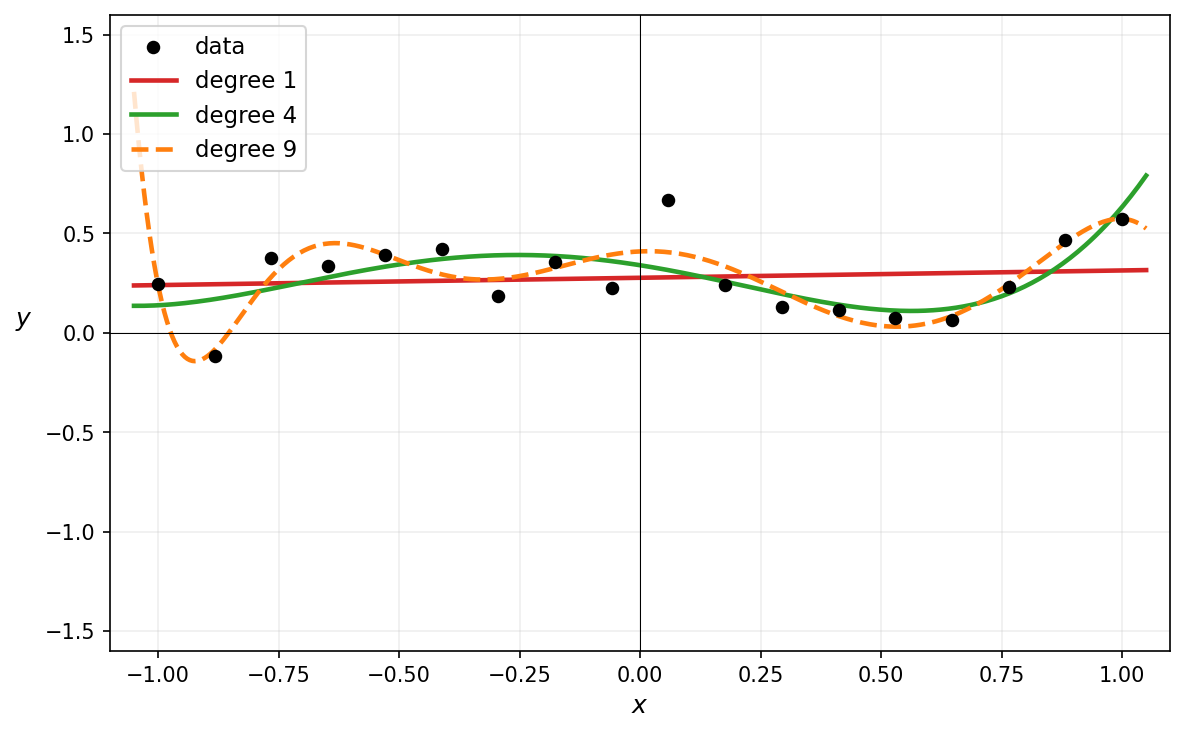
\includegraphics[width=0.88\textwidth]{figures/fig05_poly_regression.png}
  \caption{Polynomial regression on 13 noisy samples of $\sin(2\pi x)$.
    Degree~1 (red) underfits --- the linear model cannot capture the
    oscillatory signal.
    Degree~5 (green) balances bias and variance well.
    Degree~12 (orange, dashed) overfits --- it chases every data point
    and diverges wildly near the boundary.}
\end{figure}

\subsection*{Python: why exact fitting fails when $N \gg d$}
\begin{lstlisting}
import numpy as np

rng = np.random.default_rng(0)
N, d = 30, 3
x = np.linspace(-1, 1, N)
y = 2*x**2 - x + 1 + 0.3*rng.standard_normal(N)   # noisy quadratic

# Exact system: N equations, d+1 unknowns
print(f"{N} equations, {d+1} unknowns -> overdetermined, generally no exact solution")

# Least-squares fit (exact solution replaced by best approximation)
X = np.column_stack([x**k for k in range(d+1)])     # Vandermonde matrix
beta, res, rank, sv = np.linalg.lstsq(X, y, rcond=None)
print(f"fitted coefficients: {beta}")
print(f"residual ||Xbeta - y||: {np.linalg.norm(X @ beta - y):.4f}")
\end{lstlisting}

% ----- Page 23 -------------------------------------------------------
\subsection*{Matrix form and normal equations}

Encode the unknowns, data, and observations as vectors and a matrix:
\begin{align*}
  \beta &= (a_0, a_1, \ldots, a_d)^T \in \mathbb{R}^{d+1}
           &&\text{(polynomial coefficients as a vector)}\\
  X &= \begin{pmatrix}
         1 & x_1 & x_1^2 & \cdots & x_1^d \\
         \vdots & & & & \vdots \\
         1 & x_N & x_N^2 & \cdots & x_N^d
       \end{pmatrix} \in \mathbb{R}^{N\times(d+1)}
       &&\text{(feature / Vandermonde matrix)}\\
  y &= (y_1, \ldots, y_N)^T \in \mathbb{R}^N
       &&\text{(true values)}
\end{align*}

\begin{remark}[Vandermonde matrix]
  $X$ is a \emph{Vandermonde matrix}: each row $i$ evaluates the monomials
  $1, x, x^2, \ldots, x^d$ at $x_i$.  The same structure appears in
  polynomial interpolation, discrete Fourier transforms, and spectral
  methods.
\end{remark}

The exact fitting requirement $p(x_i) = y_i$ for all $i$ is:
\begin{equation}\label{eq:polyreg-matrix}
  \tag{$*$} X\beta = y,
  \qquad X \in \mathbb{R}^{N\times(d+1)},\;
  \beta \in \mathbb{R}^{d+1},\;
  y \in \mathbb{R}^N.
\end{equation}
In most cases \eqref{eq:polyreg-matrix} has no solution ($y \notin \operatorname{im}X$).

\medskip\noindent
Instead, solve the \textbf{normal equations}:
\begin{equation}\label{eq:normal}
  \tag{$**$} X^T X\,\beta = X^T y.
\end{equation}
$X^TX$ is $(d+1)\times(d+1)$ and likely invertible, giving $\beta = (X^TX)^{-1}X^Ty$.

\begin{remark}[Why the normal equations work --- forward pointer]
  Equation~\eqref{eq:normal} is not a trick: it is the condition
  $y - X\beta \perp \operatorname{im}X$, i.e.\ the residual is orthogonal
  to the column space of $X$.  The geometric interpretation --- projecting
  $y$ onto $\operatorname{im}X$ --- will be made precise once we have inner
  products and projections (\S3).
\end{remark}

\begin{remark}[Computational size reduction]
  $X$ is $N\times(d+1)$ with $N \gg d$: huge.  But $X^TX$ is only
  $(d+1)\times(d+1)$, independent of $N$.  Solving \eqref{eq:normal}
  instead of \eqref{eq:polyreg-matrix} is not only geometrically
  justified --- it is why least-squares regression is computationally
  tractable for large datasets.
\end{remark}

\subsection*{Python: Vandermonde matrix and normal equations}
\begin{lstlisting}
import numpy as np

rng = np.random.default_rng(0)
N, d = 30, 3
x = np.linspace(-1, 1, N)
y = 2*x**2 - x + 1 + 0.3*rng.standard_normal(N)

# Build Vandermonde (feature) matrix explicitly
X = np.column_stack([x**k for k in range(d + 1)])  # shape (N, d+1)
print("X shape:", X.shape)        # (30, 4)
print("X^T X shape:", (X.T @ X).shape)  # (4, 4) -- much smaller

# Solve normal equations
beta_normal = np.linalg.solve(X.T @ X, X.T @ y)

# Compare with numpy's least-squares solver
beta_lstsq, _, _, _ = np.linalg.lstsq(X, y, rcond=None)

print("normal equations:", beta_normal)
print("lstsq:           ", beta_lstsq)   # should match
\end{lstlisting}

% ----- Page 24 (bridge) -----------------------------------------------
\subsection*{From polynomial regression to inner products}

To minimise $\|X\beta - y\|$ we need a notion of distance: $\|a - b\|$
measures how close $a$ is to $b$.  The norm $\|X\beta - y\|$ we want to
minimise is $\sqrt{\langle X\beta - y,\, X\beta - y\rangle}$ under the
standard inner product on $\mathbb{R}^N$ --- the abstract definition below
directly powers this computation.

Thus, we don't need merely vector spaces; we need vector spaces
\textbf{with inner products and norms}.

% ============================================================
\section{Inner Products and Norms (\S2.1)}
% ============================================================
% Pages 24--

\subsection*{Definition and axioms}

\textbf{Toy example.}  $\mathbb{R}^2$ with the usual dot product:
$v = (a, b)$, $\|v\|^2 = a^2 + b^2 = v \cdot v$.

\begin{definition}[Inner product]
  Let $V$ be a vector space over $F = \mathbb{R}$ or $\mathbb{C}$.
  An \emph{inner product} on $V$ is a function
  $\langle\cdot,\cdot\rangle : V \times V \to F$ satisfying:
  \begin{enumerate}
    \item \textbf{Positivity} (positive definiteness):
      $\langle v, v\rangle \geq 0\ \forall\,v \in V$,
      with $\langle v, v\rangle = 0 \Leftrightarrow v = 0$.
    \item \textbf{Linearity in the first argument}:
      \begin{align*}
        \langle u + v,\, w\rangle &= \langle u, w\rangle + \langle v, w\rangle
          &&\forall\, u,v,w \in V,\\
        \langle \lambda u,\, v\rangle &= \lambda\langle u, v\rangle
          &&\forall\, \lambda \in F,\; u,v \in V.
      \end{align*}
    \item \textbf{Symmetry}:
      $\langle u, v\rangle = \langle v, u\rangle$ if $F = \mathbb{R}$;
      \quad
      $\langle u, v\rangle = \overline{\langle v, u\rangle}$
      if $F = \mathbb{C}$ (Hermitian symmetry).
  \end{enumerate}
\end{definition}

\begin{remark}[Linearity convention]
  Axiom~2 places linearity in the \emph{first} argument.  Physicists
  (Dirac bra-ket notation) conventionally put linearity in the second;
  mathematicians in the first.  Both conventions appear in standard
  references --- always check which one is in use.
\end{remark}

\begin{remark}[Conjugate-linearity in the second argument]
  Axioms~2 and~3 together imply:
  \[
    \langle u,\, \lambda v\rangle = \bar\lambda\,\langle u, v\rangle
    \quad \forall\,\lambda \in F.
  \]
  For $F = \mathbb{R}$ this is ordinary linearity; for $F = \mathbb{C}$
  it is \emph{conjugate-linearity} (sesquilinearity).
  The inner product is \emph{bilinear} only over $\mathbb{R}$.
\end{remark}

\subsection*{Python: inner product axioms}
\begin{lstlisting}
import numpy as np

def inner(u, v, W=None):
    """Standard (W=None) or weighted inner product u^T W v on R^n."""
    if W is None:
        return float(u @ v)
    return float(u @ W @ v)

u = np.array([1., 2., 3.])
v = np.array([4., 5., 6.])
W = np.diag([1., 2., 3.])        # positive definite weight matrix

print("standard <u,v>:", inner(u, v))
print("weighted <u,v>:", inner(u, v, W))

# Verify axioms for weighted inner product
print("positivity <u,u> >= 0:", inner(u, u, W) >= 0)   # True
print("symmetry <u,v>==<v,u>:", np.isclose(inner(u, v, W), inner(v, u, W)))  # True
lam = 3.0
print("linearity:", np.isclose(inner(lam*u, v, W), lam * inner(u, v, W)))    # True
\end{lstlisting}

% ----- Page 25 -------------------------------------------------------
\subsection*{Examples of inner products}

\begin{example}[Euclidean inner product on $\mathbb{R}^n$]
  \[
    \langle (x_1,\ldots,x_n)^T,\, (y_1,\ldots,y_n)^T\rangle
    = \sum_{i=1}^n x_i y_i.
  \]
\end{example}

\begin{example}[Weighted Euclidean inner product]
  If $c_1,\ldots,c_n > 0$, then
  $\langle x, y\rangle_c = \sum_{i=1}^n c_i x_i y_i$
  defines an inner product on $\mathbb{R}^n$.
  \begin{remark}[Connection to weighted regression]
    This is the inner product underlying \emph{weighted least squares}:
    setting $c_i$ to the confidence in data point $i$ assigns higher
    weight to more reliable observations.  The normal equations
    $X^TXb = X^Ty$ become $X^TCXb = X^TCy$ with diagonal weight matrix
    $C = \operatorname{diag}(c_1,\ldots,c_N)$.
  \end{remark}
\end{example}

\begin{example}[Inner products on $\mathcal{P}_n$]
  \leavevmode
  \begin{itemize}
    \item $\langle p, q\rangle = p(0)q(0) + \displaystyle\int_{-1}^1 p'(x)q'(x)\,dx$.
    \item $\langle p, q\rangle = \displaystyle\int_0^\infty p(x)q(x)e^{-x}\,dx$
          \quad ($L^2$ with exponential weight).
    \item Via the isomorphism $\phi(p) = (a_0,a_1,\ldots,a_n)^T$:
          $\langle p, q\rangle = \phi(p)\cdot\phi(q)$
          (standard dot product on $\mathbb{R}^{n+1}$).
  \end{itemize}
  \begin{proof}[Positivity check for the first variant]
    $\langle p, p\rangle = p(0)^2 + \int_{-1}^1 (p')^2\,dx = 0$
    requires $p(0) = 0$ and $p'(x) = 0$ for all $x \in [-1,1]$,
    which forces $p = 0$.  So the definiteness axiom holds.
  \end{proof}
\end{example}

\begin{definition}[Inner product space]
  An \emph{inner product space} is a vector space $V$ equipped with an
  inner product.
\end{definition}

\begin{proposition}[3.1.1]
  \leavevmode
  \begin{enumerate}
    \item[(a)] For any fixed $u \in V$, the map $f(v) = \langle v, u\rangle : V \to F$
               is a linear functional.
    \item[(b)] $\langle 0, v\rangle = 0$ and $\langle v, 0\rangle = 0$ for all $v \in V$.
  \end{enumerate}
\end{proposition}
\begin{proof}
  (a) follows directly from axiom~2 (linearity in the first argument).

  (b) $\langle 0, v\rangle = \langle 0\cdot u, v\rangle = 0\cdot\langle u, v\rangle = 0$
  for any $u \in V$.
  For the second: $\langle v, 0\rangle = \overline{\langle 0, v\rangle} = \bar{0} = 0$
  by symmetry/Hermitian symmetry.
\end{proof}

\subsection*{Python: polynomial inner products}
\begin{lstlisting}
import numpy as np
from scipy.integrate import quad

# Two polynomials: p = 1 + 2x + x^2, q = x - x^2
# Represented as coefficient vectors (a0, a1, a2)
p_c = np.array([1., 2., 1.])
q_c = np.array([0., 1., -1.])

# Inner product via phi isomorphism (coefficient dot product)
print("coeff dot <p,q>:", p_c @ q_c)   # = 0*1 + 1*2 + (-1)*1 = 1

# L^2 weighted inner product: integral_0^inf p(x)q(x)e^{-x} dx
p = np.poly1d(p_c[::-1])   # np.poly1d uses highest-degree first
q = np.poly1d(q_c[::-1])
val, _ = quad(lambda x: p(x) * q(x) * np.exp(-x), 0, np.inf)
print("L2 weighted <p,q>:", round(val, 6))  # different value: different inner product
\end{lstlisting}

% ----- Page 26 -------------------------------------------------------
\subsection*{Derived properties, norm, orthogonality}

The following properties are consequences of the axioms (not additional
assumptions):
\begin{itemize}
  \item[(c)] $\langle u, v+w\rangle = \langle u,v\rangle + \langle u,w\rangle$,
             $\quad\forall\, u,v,w\in V$.
  \item[(d)] $\langle u, \lambda v\rangle = \bar\lambda\,\langle u,v\rangle$,
             $\quad\forall\,\lambda\in F,\; u,v\in V$.
\end{itemize}
(Both follow from axioms~2 and~3: apply linearity in the first argument to
$\langle v+w, u\rangle$ and $\langle \lambda v, u\rangle$, then use symmetry.)

\begin{definition}[Norm induced by an inner product]
  \[
    \|v\|^2 = \langle v, v\rangle, \qquad \|v\| = \sqrt{\langle v, v\rangle}.
  \]
\end{definition}

\begin{proposition}[3.1.2]
  For any $v \in V$ and $\lambda \in F$:
  \begin{enumerate}
    \item[(a)] $\|v\| = 0 \Longleftrightarrow v = 0$.
    \item[(b)] $\|\lambda v\| = |\lambda|\,\|v\|$.
  \end{enumerate}
\end{proposition}
\begin{proof}
  (a) $\|v\| = 0 \Leftrightarrow \langle v,v\rangle = 0 \Leftrightarrow v = 0$
  by the positivity axiom.

  (b) $\|\lambda v\|^2 = \langle \lambda v, \lambda v\rangle
      = \lambda\,\langle v, \lambda v\rangle
      = \lambda\bar\lambda\,\langle v,v\rangle
      = |\lambda|^2\|v\|^2$.
  Taking square roots gives $\|\lambda v\| = |\lambda|\,\|v\|$.
\end{proof}

\begin{definition}[Orthogonality]
  $u, v \in V$ are \emph{orthogonal}, written $u \perp v$, if
  $\langle u, v\rangle = 0$.
\end{definition}

\begin{example}
  $0$ is orthogonal to every $v \in V$ (by Prop~3.1.1(b)).
  It is the \emph{only} vector orthogonal to itself: if $\langle v,v\rangle = 0$
  then $v = 0$ by positivity.
\end{example}

\begin{theorem}[3.1.3 — Pythagorean theorem]
  If $u \perp v$, then $\|u + v\|^2 = \|u\|^2 + \|v\|^2$.
\end{theorem}
\begin{proof}
  \[
    \|u+v\|^2
    = \langle u+v,\, u+v\rangle
    = \|u\|^2 + \langle u,v\rangle + \langle v,u\rangle + \|v\|^2
    = \|u\|^2 + 0 + 0 + \|v\|^2. \qedhere
  \]
\end{proof}

\begin{definition}[Orthogonal projection onto $v \neq 0$]
  \[
    \operatorname{proj}_v(u)
    = \frac{\langle u, v\rangle}{\|v\|^2}\,v.
  \]
\end{definition}

\begin{remark}[Why this formula]
  $\operatorname{proj}_v(u)$ is the unique scalar multiple of $v$ closest
  to $u$.  The residual $u - \operatorname{proj}_v(u)$ is orthogonal to $v$:
  \[
    \Bigl\langle u - \tfrac{\langle u,v\rangle}{\|v\|^2}v,\; v\Bigr\rangle
    = \langle u,v\rangle - \tfrac{\langle u,v\rangle}{\|v\|^2}\|v\|^2 = 0.
  \]
  This residual-orthogonality is the same condition as the normal equations
  $X^TXb = X^Ty$: the projection of $y$ onto $\operatorname{im}X$ makes
  the residual $y - Xb$ orthogonal to every column of $X$.
\end{remark}

\begin{figure}[h!]
  \centering
  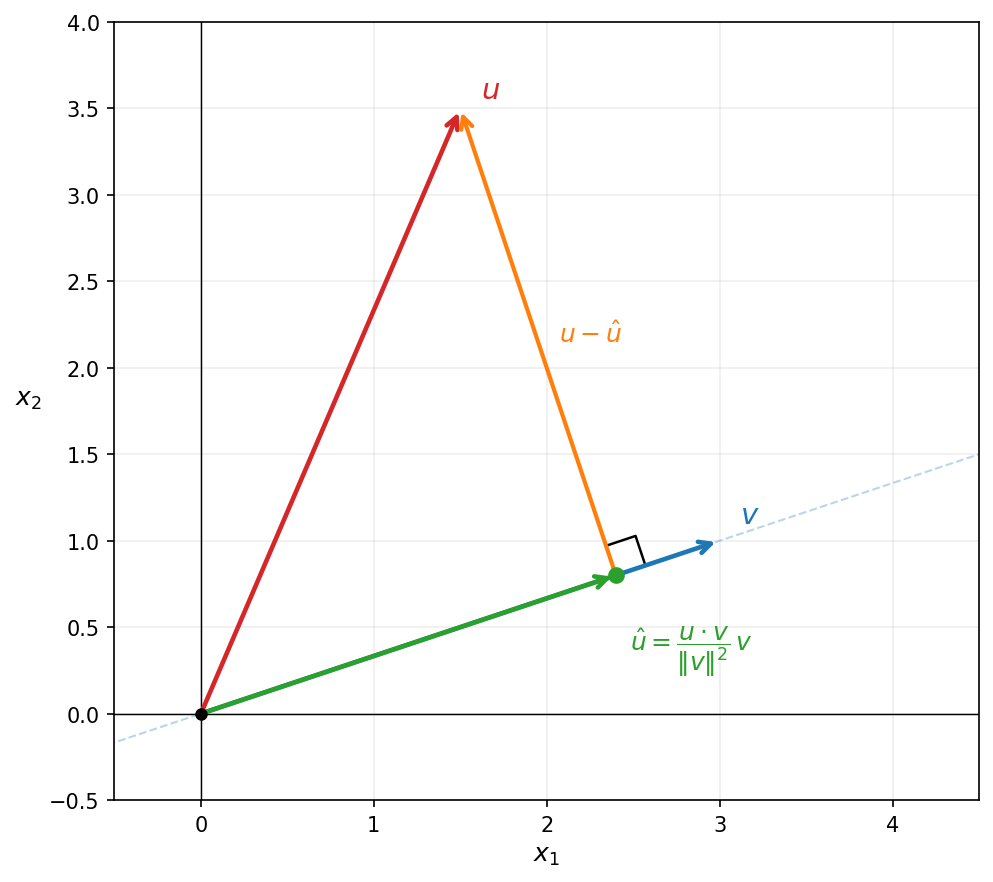
\includegraphics[width=0.6\textwidth]{figures/fig04_projection.png}
  \caption{Orthogonal projection of $u$ onto $v$ in $\mathbb{R}^2$.
    The projection $\hat u = \frac{\langle u,v\rangle}{\|v\|^2}v$ is the
    foot of the perpendicular from $u$ to the line spanned by $v$;
    the residual $u - \hat u$ is orthogonal to $v$.}
\end{figure}

\begin{remark}[Geometry as a guide to abstraction]
  Figure above depicts projection in $\mathbb{R}^2$, where we can draw
  arrows and right angles.  Other vector spaces --- polynomials, matrices,
  sequences --- do not come with a ready-made picture.  Yet the formula
  $\hat u = \frac{\langle u,v\rangle}{\|v\|^2}v$ holds in \emph{any}
  inner product space, and the residual is always perpendicular to $v$ in
  that space's inner product.  The power of the axiomatic framework is
  precisely this: we develop intuition in $\mathbb{R}^2$, encode it in
  abstract algebra, and then apply it for free in every vector space at once.
\end{remark}

\subsection*{Python: projection and orthogonality of residual}
\begin{lstlisting}
import numpy as np

u = np.array([3., 2.])
v = np.array([1., 0.])          # project onto x-axis

proj = (np.dot(u, v) / np.dot(v, v)) * v
residual = u - proj

print("proj_v(u):", proj)                              # [3. 0.]
print("residual:", residual)                           # [0. 2.]
print("residual perp v:", np.isclose(np.dot(residual, v), 0))  # True
print("Pythagorean check:", np.isclose(
    np.dot(u, u),
    np.dot(proj, proj) + np.dot(residual, residual)))  # True
\end{lstlisting}

% ----- Page 27 -------------------------------------------------------
\begin{proposition}[3.1.4]
  If $v \neq 0$, then $\operatorname{proj}_v(u)$ and
  $w = u - \operatorname{proj}_v(u)$ are orthogonal for all $u \in V$.
\end{proposition}
\begin{proof}
  \[
    \bigl\langle u - \operatorname{proj}_v(u),\; v\bigr\rangle
    = \langle u, v\rangle
      - \frac{\langle u,v\rangle}{\|v\|^2}\,\langle v,v\rangle
    = \langle u,v\rangle - \langle u,v\rangle = 0. \qedhere
  \]
\end{proof}

\begin{theorem}[3.1.5 --- Cauchy--Schwarz]
  For all $u, v \in V$:
  \[
    |\langle u, v\rangle| \leq \|u\|\,\|v\|,
  \]
  with equality if and only if $u = \lambda v$ for some $\lambda \in F$.
\end{theorem}
\begin{proof}
  If $v = 0$ both sides are $0$.  Assume $v \neq 0$.
  For any $\lambda \in \mathbb{R}$, positivity gives
  \[
    0 \leq \|u - \lambda v\|^2
      = \|u\|^2 - 2\lambda\operatorname{Re}\langle u,v\rangle
        + \lambda^2\|v\|^2.
  \]
  This is a quadratic in $\lambda$ that is always $\geq 0$, so its
  discriminant is non-positive:
  \[
    4(\operatorname{Re}\langle u,v\rangle)^2 - 4\|u\|^2\|v\|^2 \leq 0
    \;\Longrightarrow\;
    |\langle u,v\rangle|^2 \leq \|u\|^2\|v\|^2.
  \]
  Equality holds iff the quadratic has a real root, i.e.\ $u = \lambda v$.
\end{proof}

\begin{theorem}[3.1.6 --- Triangle Inequality]
  For all $u, v \in V$: $\|u + v\| \leq \|u\| + \|v\|$,
  with equality iff $u = \lambda v$ for some $\lambda > 0$.
\end{theorem}
\begin{proof}
  \[
    \|u+v\|^2
    = \|u\|^2 + 2\operatorname{Re}\langle u,v\rangle + \|v\|^2
    \leq \|u\|^2 + 2|\langle u,v\rangle| + \|v\|^2
    \leq \|u\|^2 + 2\|u\|\|v\| + \|v\|^2
    = \bigl(\|u\| + \|v\|\bigr)^2,
  \]
  where the last inequality is Cauchy--Schwarz.  Take square roots.
\end{proof}

\begin{exercise}[Parallelogram equality]
  Show that for all $u, v \in V$:
  \[
    \|u+v\|^2 + \|u-v\|^2 = 2\|u\|^2 + 2\|v\|^2.
  \]
\end{exercise}

\begin{remark}[Parallelogram law characterises inner product norms]
  The Jordan--von Neumann theorem states that a normed space has its norm
  induced by an inner product \emph{if and only if} the parallelogram
  equality holds.  Consequently, $L^p$ norms for $p \neq 2$ do \emph{not}
  come from inner products --- a fact that matters in functional analysis,
  robust regression, and any setting where $\|\cdot\|_p$ with $p \neq 2$
  appears.
\end{remark}

\begin{definition}[Orthogonal complement]
  If $U \leq V$, the \emph{orthogonal complement} of $U$ is
  \[
    U^\perp = \{v \in V : \langle v, u\rangle = 0\; \forall\, u \in U\}.
  \]
\end{definition}

% ----- Page 28 -------------------------------------------------------
\subsection*{Back to polynomial regression: why the normal equations work}

Let $U = \operatorname{im}X \leq \mathbb{R}^N$ be the column space of the
feature matrix.  We want $\hat\beta$ minimising $\|y - X\beta\|$.

\medskip\noindent
\textbf{Geometric argument.}
Project $y$ onto $U$: the projection $\hat{y} = \operatorname{proj}_U(y)$
always exists (inner product space, finite dimension) and is unique.
By definition of projection, $y - \hat{y} \perp U$, i.e.\
$\langle y - \hat{y}, Xv\rangle = 0$ for all $v\in\mathbb{R}^{d+1}$.
Write $\hat{y} = X\hat\beta$; then
\[
  \langle y - X\hat\beta,\, Xv\rangle = 0
  \;\;\forall\, v
  \;\;\Longrightarrow\;\;
  X^T(y - X\hat\beta) = 0
  \;\;\Longrightarrow\;\;
  X^TX\hat\beta = X^Ty.
\]
The minimiser satisfies the normal equations.  $\hat{y}$ is unique;
$\hat\beta$ need not be if $\ker X \neq \{0\}$.

\medskip\noindent
\textbf{Algebraic argument (normal equations always have a solution).}
It is not obvious that $X^Ty \in \operatorname{im}(X^TX)$.  The following
lemma shows it.

\begin{proposition}[$\ker(X^TX) = \ker(X)$]
  For any $X \in \mathbb{R}^{N\times(d+1)}$:
  \[
    \ker(X^TX) = \ker(X).
  \]
\end{proposition}
\begin{proof}
  $\ker(X) \subseteq \ker(X^TX)$: if $Xv = 0$ then $X^TXv = 0$. \\
  $\ker(X^TX) \subseteq \ker(X)$: if $X^TXv = 0$, then
  $\|Xv\|^2 = \langle Xv, Xv\rangle = v^TX^TXv = 0$,
  so $Xv = 0$.
\end{proof}

\begin{corollary}
  $\operatorname{im}(X^TX) = \operatorname{im}(X^T)$, so
  $X^Ty \in \operatorname{im}(X^TX)$ for every $y$.
  Hence the normal equations always have a solution.
\end{corollary}
\begin{proof}
  By the Im-Ker Theorem,
  $\operatorname{rk}(X^TX) = \operatorname{rk}(X) = \operatorname{rk}(X^T)$.
  Since $\operatorname{im}(X^TX) \subseteq \operatorname{im}(X^T)$ and both
  have the same dimension, they are equal.
  Finally $X^Ty = X^T \cdot y \in \operatorname{im}(X^T)$ trivially.
\end{proof}

\medskip\noindent
The complete chain of equivalences:
\[
  \|y - X\beta\| \to \min
  \;\Longleftrightarrow\;
  y - X\beta \perp \operatorname{im}X
  \;\Longleftrightarrow\;
  X^TX\beta = X^Ty.
\]

\begin{definition}[Hat matrix / projection matrix]
  The \emph{hat matrix}
  $H = X(X^TX)^{-1}X^T$ (when $X$ has full column rank) satisfies
  $\hat{y} = Hy$ and:
  \[
    H^2 = H \quad\text{(idempotent)}, \qquad H^T = H \quad\text{(symmetric)}.
  \]
  These two properties characterise orthogonal projections.
\end{definition}

\subsection*{Python: hat matrix and projection}
\begin{lstlisting}
import numpy as np

rng = np.random.default_rng(0)
N, d = 30, 3
x  = np.linspace(-1, 1, N)
y  = 2*x**2 - x + 1 + 0.3*rng.standard_normal(N)
X  = np.column_stack([x**k for k in range(d + 1)])

# Hat matrix
H     = X @ np.linalg.solve(X.T @ X, X.T)
y_hat = H @ y                         # projection of y onto im X
resid = y - y_hat

print("H^2 = H:", np.allclose(H @ H, H))         # True
print("H^T = H:", np.allclose(H.T, H))            # True
print("resid perp im X:", np.allclose(X.T @ resid, 0))  # True (normal eqs)
print("||resid||:", np.linalg.norm(resid).round(4))
\end{lstlisting}

% ----- Page 29 -------------------------------------------------------
\subsection*{Completing the normal equations derivation}

\begin{lemma}\label{lem:zero-inner}
  For a fixed $a \in \mathbb{R}^n$: if $\langle a, b\rangle = 0$ for all
  $b \in \mathbb{R}^n$, then $a = 0$.
\end{lemma}
\begin{proof}
  Take $b = a$: then $\langle a, a\rangle = 0$, so $a = 0$ by positivity.
\end{proof}

\noindent
Applying Lemma~\ref{lem:zero-inner}: from
$\langle X^TX\beta - X^Ty,\, v\rangle = 0$ for all $v \in \mathbb{R}^{d+1}$
we conclude $X^TX\beta - X^Ty = 0$, i.e.\ $X^TX\beta = X^Ty$.

\medskip\noindent
\textbf{Question:} in most cases $X^TX$ has an inverse.  Why?

\begin{proposition}[Invertibility of $X^TX$]
  $X^TX$ is invertible if and only if $\operatorname{rk}(X) = d+1$
  (columns of $X$ are linearly independent).
\end{proposition}
\begin{proof}
  $X^TX$ is invertible iff $\ker(X^TX) = \{0\}$ iff $\ker(X) = \{0\}$
  (by the proposition on page~28) iff $\operatorname{rk}(X) = d+1$.
\end{proof}

\begin{remark}[When is this satisfied?]
  The columns of $X$ are linearly independent when the nodes $x_1,\ldots,x_N$
  are \emph{distinct} and $N \geq d+1$.  A Vandermonde matrix with distinct
  nodes is always full rank (its determinant is $\prod_{i<j}(x_j-x_i)\neq 0$).
  ``In most cases'' means precisely this: the degenerate cases are repeated
  $x$-values or fewer data points than parameters.
\end{remark}

\noindent
\textbf{Summary.}  The full chain:
\[
  \|y - X\beta\| \to \min
  \;\Longleftrightarrow\;
  y - X\beta \perp \operatorname{im}X
  \;\Longleftrightarrow\;
  X^TX\beta = X^Ty
  \;\xRightarrow{\,X^TX \text{ invertible}\,}\;
  \beta^* = (X^TX)^{-1}X^Ty.
\]
This closes the loop opened on page~23.

\subsection*{Python: rank of $X^TX$ for good vs.\ degenerate data}
\begin{lstlisting}
import numpy as np

d = 3   # degree

# Generic case: distinct nodes, N >> d+1
x_good = np.linspace(-1, 1, 30)
X_good = np.column_stack([x_good**k for k in range(d + 1)])
print("rank(X^TX) good:", np.linalg.matrix_rank(X_good.T @ X_good))  # 4

# Degenerate: all nodes the same
x_bad = np.zeros(30)
X_bad = np.column_stack([x_bad**k for k in range(d + 1)])
print("rank(X^TX) bad:", np.linalg.matrix_rank(X_bad.T @ X_bad))     # 1

# Degenerate: fewer points than parameters
x_few = np.array([-1., 0., 1.])   # only 3 points, d+1 = 4 unknowns
X_few = np.column_stack([x_few**k for k in range(d + 1)])
print("rank(X^TX) few:", np.linalg.matrix_rank(X_few.T @ X_few))     # 3 < 4
\end{lstlisting}

% ============================================================
\section{Im-Ker Theorem: Full Proof}
% ============================================================
% Pages 30--31

\subsection*{Terminology and statement}

Going back to Theorem~1.6 (Im-Ker / Rank-Nullity), we now give the full
proof in the abstract linear map setting.

\medskip\noindent
Recall the terminology:
\begin{align*}
  \operatorname{im}A &= \operatorname{col}(A) = \text{column space of }A,\\
  \operatorname{im}A^T &= \operatorname{row}(A) = \text{row space of }A,\\
  \operatorname{null}A &= \dim\ker A \quad\text{(``nullity'' of }A),\\
  \ker A &= \text{``null-space'' of }A.
\end{align*}

\begin{remark}[Row rank equals column rank]
  The equality $\operatorname{rk}A = \dim\operatorname{im}A
  \stackrel{?}{=} \dim\operatorname{im}A^T$ is a genuine theorem, not
  obvious.  It follows from combining the Im-Ker Theorem applied to both
  $A$ and $A^T$ with the identity $\operatorname{rk}(A^TA) = \operatorname{rk}(A)$
  proved on page~28 (via $\ker(A^TA) = \ker(A)$).
\end{remark}

\begin{theorem}[1.6, matrix form]
  For any $A \in \mathbb{R}^{m \times n}$:
  $\operatorname{rk}A + \operatorname{null}A = n$.
\end{theorem}

\begin{theorem}[1.6, linear transform form --- Im-Ker Theorem]
  For any $L \in \mathcal{L}(V, W)$:
  $\dim\operatorname{im}L + \dim\ker L = \dim V$.
\end{theorem}

\begin{proof}
  \textbf{Proof strategy:} split $V = \ker L \oplus C$ (complement),
  then show $\{L(u_1),\ldots,L(u_r)\}$ is a basis for $\operatorname{im}L$.

  Let $V_1 = \ker L \leq V$ and $\dim V_1 = k \leq n = \dim V$.
  Pick a basis $\{b_1,\ldots,b_k\}$ for $V_1$.
  By the Steinitz extension (pages~18--19), extend to a basis of $V$
  by adjoining $\{u_1,\ldots,u_r\}$ with $k + r = n$:
  \[
    V = \langle b_1\rangle\oplus\cdots\oplus\langle b_k\rangle
        \oplus\langle u_1\rangle\oplus\cdots\oplus\langle u_r\rangle.
  \]
  Every $v \in V$ writes uniquely as
  $v = \sum_{i=1}^k \lambda_i b_i + \sum_{j=1}^r \mu_j u_j$.
  \emph{(Proof continues on page~31.)}
\end{proof}

\subsection*{Python: row rank equals column rank}
\begin{lstlisting}
import numpy as np
rng = np.random.default_rng(0)

A = rng.standard_normal((5, 8))
print("col rank (rank of A):  ", np.linalg.matrix_rank(A))    # e.g. 5
print("row rank (rank of A^T):", np.linalg.matrix_rank(A.T))  # same

# True for any matrix -- a non-trivial theorem
B = rng.standard_normal((7, 3))
print("col rank:", np.linalg.matrix_rank(B))    # 3
print("row rank:", np.linalg.matrix_rank(B.T))  # 3
\end{lstlisting}

% ----- Page 31 -------------------------------------------------------
\subsection*{Proof of Im-Ker Theorem (conclusion)}

\begin{proof}[Proof (continued from page~30)]
  Let $V_1 = \ker L$ and $V_2 = \operatorname{span}\{u_1,\ldots,u_r\}$,
  so that $V = V_1 \oplus V_2$ (direct sum from the basis construction).

  \textbf{Step 1: $\operatorname{im}L = \operatorname{span}\{L(u_1),\ldots,L(u_r)\}$.}
  Since $b_i \in \ker L$, applying $L$ to the decomposition of $v$ gives
  \[
    L(v) = \sum_{i=1}^k \lambda_i \underbrace{L(b_i)}_{=\,0}
           + \sum_{j=1}^r \mu_j L(u_j)
         = \sum_{j=1}^r \mu_j L(u_j).
  \]
  So every $L(v) \in \operatorname{span}\{L(u_1),\ldots,L(u_r)\}$, giving
  $\operatorname{im}L \subseteq \operatorname{span}\{L(u_1),\ldots,L(u_r)\}$;
  the reverse inclusion is immediate.

  \textbf{Step 2: $\{L(u_1),\ldots,L(u_r)\}$ is linearly independent.}
  Suppose $\sum_{j=1}^r \mu_j L(u_j) = 0$.  Then
  $L\!\bigl(\sum_j \mu_j u_j\bigr) = 0$, so
  $u := \sum_j \mu_j u_j \in \ker L = V_1$.
  But also $u \in V_2$ by construction.
  Since $V = V_1 \oplus V_2$ we have $V_1 \cap V_2 = \{0\}$, so $u = 0$.
  The $u_j$ are linearly independent, so $\mu_j = 0$ for all $j$.

  \textbf{Conclusion.}  Steps 1 and 2 together show
  $\{L(u_1),\ldots,L(u_r)\}$ is a \emph{basis} for $\operatorname{im}L$,
  giving $\dim\operatorname{im}L = r$.
  With $\dim\ker L = k$ and $k + r = n = \dim V$:
  \[
    \dim\operatorname{im}L + \dim\ker L = r + k = n = \dim V. \qedhere
  \]
\end{proof}

\begin{remark}[Connection to column reduction]
  The proof constructs exactly what the algorithm of pages~16--17 computes:
  $V_2 = \operatorname{span}\{u_1,\ldots,u_r\}$ corresponds to the
  \emph{pivot columns} (a basis for $\operatorname{im}A$), while the
  \emph{free columns} (zero top-block columns) generate $\ker A$.
  The abstract decomposition $V = V_1 \oplus V_2$ is what the column
  reduction algorithm realises concretely.
\end{remark}

\begin{remark}[First isomorphism theorem]
  The proof shows that the restricted map
  $L|_{V_2} : V_2 \to \operatorname{im}L$ is an isomorphism.
  Equivalently, $L$ induces a well-defined bijection on the
  \emph{quotient space} $V/\ker L \xrightarrow{\;\sim\;} \operatorname{im}L$,
  which is the \textbf{first isomorphism theorem} for vector spaces.
  The dimension count $\dim\operatorname{im}L = \dim V - \dim\ker L$ is
  its immediate corollary.
\end{remark}

% ----- Page 32 -------------------------------------------------------
\subsection*{Row space, orthogonal complements, and the four subspaces}

Recall that $Ax$ is a linear combination of the columns of $A$, but also:
\[
  Ax = \begin{pmatrix}a_1^T x\\\vdots\\a_m^T x\end{pmatrix},
  \qquad a_i = i\text{-th row of }A = i\text{-th column of }A^T.
\]
Hence
\[
  Ax = 0
  \;\Longleftrightarrow\;
  a_i^T x = 0\;\;\forall\,i
  \;\Longleftrightarrow\;
  x \perp \langle a_1,\ldots,a_m\rangle = \operatorname{row}(A).
\]
So $\ker A = \bigl(\operatorname{row}(A)\bigr)^\perp$ inside $\mathbb{R}^m$.

\begin{proposition}[3.1.7, Homework]
  $U^\perp \leq V$.
\end{proposition}
\begin{proof}
  $\langle 0, u\rangle = 0$ for all $u$, so $0 \in U^\perp$.
  If $v,w \in U^\perp$ and $\lambda \in F$, then for all $u \in U$:
  $\langle v+w, u\rangle = \langle v,u\rangle + \langle w,u\rangle = 0$
  and $\langle \lambda v, u\rangle = \lambda\langle v,u\rangle = 0$.
  So $U^\perp$ is closed under addition and scaling.
\end{proof}

\begin{proposition}[3.1.8, Homework]
  $V = U \oplus U^\perp$.
\end{proposition}
\begin{proof}[Proof sketch]
  \textit{$U\cap U^\perp = \{0\}$:} if $v\in U\cap U^\perp$ then
  $\langle v,v\rangle = 0$, so $v = 0$ by positivity.

  \textit{$V = U + U^\perp$:} let $\{e_1,\ldots,e_k\}$ be an orthonormal
  basis for $U$ (existence via Gram--Schmidt, \S3.2).
  For any $v\in V$, set $u = \sum_i \langle v,e_i\rangle e_i \in U$.
  Then $v - u \perp e_j$ for each $j$ (direct computation), so
  $v - u \in U^\perp$ and $v = u + (v-u)$.
\end{proof}

\noindent
Taking $U = \operatorname{row}(A) \leq \mathbb{R}^m$:
\[
  \mathbb{R}^m = \operatorname{row}(A) \oplus \ker(A).
\]
Hence $m = \dim\operatorname{row}(A) + \dim\ker(A) = \dim\operatorname{row}(A) + \operatorname{null}(A)$.
By Thm~1.6, $m = \operatorname{rk}(A) + \operatorname{null}(A)$, giving:
\[
  \boxed{\operatorname{rk}(A) = \dim\operatorname{row}(A).}
  \qquad\text{(row rank = column rank)}
\]

\begin{remark}[Strang's four fundamental subspaces]
  Applying $V = U \oplus U^\perp$ to both $A$ and $A^T$ gives the full picture:
  \begin{align*}
    \mathbb{R}^m &= \operatorname{row}(A) \oplus \ker(A), \\
    \mathbb{R}^n &= \operatorname{col}(A) \oplus \ker(A^T).
  \end{align*}
  The four subspaces --- column space, row space, null space, left null
  space --- come in two orthogonal pairs, one pair in $\mathbb{R}^m$,
  one in $\mathbb{R}^n$.  Their dimensions are fixed by
  $\operatorname{rk}(A)$ alone.
\end{remark}

\begin{remark}[$V = U \oplus U^\perp$ as a recurring theme]
  This decomposition is the structural engine behind Gram--Schmidt
  (building orthonormal bases), orthogonal projections, the normal
  equations, and eventually SVD.  The fact that every subspace has an
  orthogonal complement --- and that the two together fill the whole
  space --- is what makes inner product spaces so much richer than plain
  vector spaces.
\end{remark}

\begin{figure}[h!]
  \centering
  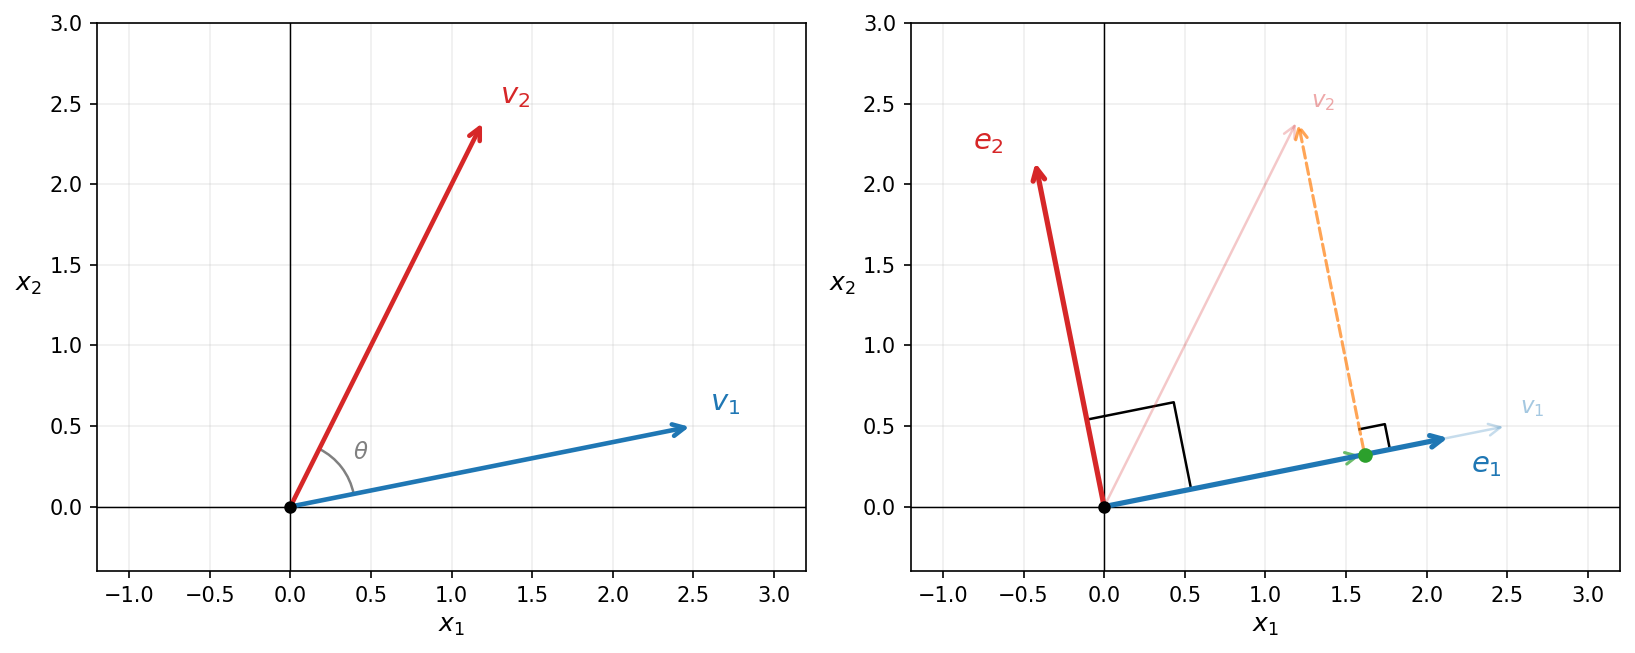
\includegraphics[width=\textwidth]{figures/fig06_gram_schmidt.png}
  \caption{Gram--Schmidt orthogonalization in $\mathbb{R}^2$.
    \emph{Left:} original vectors $v_1, v_2$ at angle $\theta$.
    \emph{Right:} the green dashed arrow is the projection of $v_2$ onto
    $e_1$; the orange dashed arrow is the residual $v_2 - \operatorname{proj}_{e_1}v_2$,
    perpendicular to $e_1$ (right-angle marker at the foot).
    Normalizing the residual gives $e_2$.}
\end{figure}

\subsection*{Python: the four fundamental subspaces are mutually orthogonal}
\begin{lstlisting}
import numpy as np
from scipy.linalg import null_space, orth

rng = np.random.default_rng(0)
A = rng.standard_normal((4, 6))      # 4x6, rank 4 generically

row_A  = orth(A.T)                   # basis for row(A)   in R^6
ker_A  = null_space(A)               # basis for ker(A)   in R^6
col_A  = orth(A)                     # basis for col(A)   in R^4
lnul_A = null_space(A.T)             # basis for ker(A^T) in R^4

print("row(A)  perp ker(A):", np.allclose(row_A.T  @ ker_A,  0))  # True
print("col(A)  perp ker(A^T):", np.allclose(col_A.T @ lnul_A, 0))  # True

# Dimension check
print(f"R^6: dim row={row_A.shape[1]}, dim ker={ker_A.shape[1]}, sum={row_A.shape[1]+ker_A.shape[1]}")   # 4+2=6
print(f"R^4: dim col={col_A.shape[1]}, dim lnul={lnul_A.shape[1]}, sum={col_A.shape[1]+lnul_A.shape[1]}") # 4+0=4
\end{lstlisting}

% ----- Page 33 (conclusion of Im-Ker section) -------------------------

\begin{theorem}[3.1.9 --- Row rank equals column rank]
  For any $A \in \mathbb{R}^{m\times n}$:
  \[
    \text{column-rank}(A) = \text{row-rank}(A) = \operatorname{rk}A,
  \]
  where column-rank$(A)$ = max $\#$ of linearly independent columns,
  and row-rank$(A)$ = max $\#$ of linearly independent rows.
\end{theorem}
\begin{proof}
  By page~32: $\mathbb{R}^m = \operatorname{row}(A)\oplus\ker(A)$, so
  $\dim\operatorname{row}(A) = m - \operatorname{null}(A)$.
  By Thm~1.6: $\operatorname{rk}(A) = m - \operatorname{null}(A)$.
  Hence $\text{row-rank}(A) = \operatorname{rk}(A) = \dim\operatorname{im}(A) = \text{column-rank}(A)$.
\end{proof}

% ============================================================
\section{Structural Properties of Linear Transformations (\S4)}
% ============================================================
% Pages 33--

\subsection*{\S4.1 Change of basis}

\textbf{Main question.}  Let $L: V \to W$ be a linear transform,
$\dim V = n$, $\dim W = m$.  Can we ``simplify'' the action of $L$ by
choosing a good basis?

\begin{remark}[What ``simpler'' means]
  The target normal forms, in increasing generality:
  \begin{itemize}
    \item \textbf{Diagonal} --- achievable when $L$ has $n$ linearly
      independent eigenvectors (diagonalisable maps, \S4.2).
    \item \textbf{Upper triangular} --- always achievable over $\mathbb{C}$
      (Schur decomposition).
    \item \textbf{Jordan normal form} --- the finest canonical form over
      $\mathbb{C}$, grouping generalised eigenvectors into Jordan blocks.
  \end{itemize}
  For now we focus on the case $V = W = \mathbb{R}^n$ and ask: in what
  basis is the matrix of $L$ simplest?
\end{remark}

\noindent
Let $A$ be the matrix of $L: x \mapsto Ax$ in the \emph{standard} basis
of $\mathbb{R}^n$.  Let $B = [b_1 \mid \cdots \mid b_n]$ be another
basis matrix (invertible, columns are the new basis vectors).

\medskip\noindent
\textbf{Change-of-basis formula.}  A vector with standard coordinates $x$
has $B$-coordinates $x' = B^{-1}x$.  Applying $L$:
\[
  x \xmapsto{L} Ax
  \;\;\Longrightarrow\;\;
  x' \xmapsto{L_B} B^{-1}AB\, x'.
\]
So the matrix of $L$ in basis $B$ is $\boxed{A_B = B^{-1}AB}$.

\begin{remark}[Similar matrices]
  Two matrices $A$ and $A_B = B^{-1}AB$ represent the \emph{same} linear
  map in different bases.  Such matrices are called \emph{similar}.
  Similarity is an equivalence relation; finding the simplest
  representative in each equivalence class is the central problem of
  \S4.
\end{remark}

\subsection*{Python: change of basis}
\begin{lstlisting}
import numpy as np

A = np.array([[2., 1.],
              [0., 3.]])        # matrix of L in standard basis

B = np.array([[1., 1.],
              [0., 1.]])        # new basis (columns are basis vectors)

A_B = np.linalg.inv(B) @ A @ B  # matrix of L in basis B
print("A in standard basis:\n", A)
print("A in new basis B:\n", A_B)

# Verify: same eigenvalues (similarity preserves eigenvalues)
print("eigenvalues of A:  ", np.linalg.eigvals(A))
print("eigenvalues of A_B:", np.linalg.eigvals(A_B))   # same
\end{lstlisting}

% ----- Page 34 -------------------------------------------------------
\subsection*{Derivation of the change-of-basis formula}

Let $P = [b_1' \mid b_2' \mid \cdots \mid b_n']$ be the change-of-basis
matrix (columns = new basis vectors, expressed in the standard basis).
A vector with standard coordinates $x$ has $B$-coordinates
$x' = P^{-1}x$; conversely $x = Px'$.

\begin{remark}[$P$ is always invertible]
  The columns of $P$ form a basis, hence are linearly independent, hence
  $P$ is square and invertible.  The change-of-basis matrix always has an
  inverse.
\end{remark}

\noindent
The commutative diagram:
\[
  \begin{array}{ccc}
    x \in \mathbb{R}^n_{\mathrm{std}} & \xrightarrow{\;A\;} &
    y \in \mathbb{R}^n_{\mathrm{std}} \\[4pt]
    {\scriptstyle P}\Big\uparrow & & \Big\uparrow{\scriptstyle P} \\[4pt]
    x' \in \mathbb{R}^n_{B} & \xrightarrow{\;A'\;} & y' \in \mathbb{R}^n_{B}
  \end{array}
\]
From $y = Ax$ and $x = Px'$, $y = Py'$:
\[
  Py' = A\,Px'
  \;\Longrightarrow\;
  y' = P^{-1}AP\,x'
  \;\Longrightarrow\;
  \boxed{A' = P^{-1}AP.}
\]
Equivalently: $A = PA'P^{-1}$, so the standard-basis matrix is recovered
from the $B$-basis matrix by conjugation with $P$.

\begin{remark}[Two equivalent forms]
  \begin{itemize}
    \item $A' = P^{-1}AP$ \quad --- matrix of $L$ in basis $B$, given standard-basis matrix $A$.
    \item $A  = PA'P^{-1}$ \quad --- standard-basis matrix, given $B$-basis matrix $A'$.
  \end{itemize}
  Students often confuse which way the $P$ goes; checking with a simple
  example (as below) is the safest remedy.
\end{remark}

\subsection*{Python: verifying $A' = P^{-1}AP$}
\begin{lstlisting}
import numpy as np

A = np.array([[3., 1.],
              [0., 2.]])           # matrix of L in standard basis

P = np.array([[1., 2.],
              [1., 3.]])           # columns = new basis vectors (invertible)

A_prime = np.linalg.inv(P) @ A @ P   # matrix of L in basis B

# Same linear map: A applied to Px' equals P times A'x'
x_prime = np.array([1., -1.])
print("A(Px') :", A @ (P @ x_prime))
print("P(A'x'):", P @ (A_prime @ x_prime))   # must match

# Similarity preserves eigenvalues
print("eig(A)      :", np.linalg.eigvals(A))
print("eig(A_prime):", np.linalg.eigvals(A_prime))   # same
\end{lstlisting}

% ============================================================
% ============================================================
\section{Eigenvalues and Diagonalization (\S4.2)}
% ============================================================
% Pages 35--

% ----- Page 35 -------------------------------------------------------

\noindent
\textbf{Central question of \S4.}  Given $A \in \mathbb{R}^{n\times n}$,
is there an invertible $P \in \mathbb{R}^{n\times n}$ such that $P^{-1}AP$
has a simpler structure --- e.g.\ diagonal, upper triangular?

\subsection*{\S4.2 Eigenvectors and eigenvalues}

\begin{definition}
  Let $L : V \to V$ be a linear transform on a vector space $V$ over $F$.
  A vector $v \neq 0$, $v \in V$ is an \emph{eigenvector} of $L$ with
  \emph{eigenvalue} $\lambda \in F$ iff
  \[
    L(v) = \lambda v.
  \]
  The condition $v \neq 0$ is essential: $L(0) = \lambda\cdot 0$ holds for
  every $\lambda$ and would make eigenvalues meaningless.
\end{definition}

\begin{example}
  $A = \begin{pmatrix}1&2\\0&3\end{pmatrix}$ has eigenvectors
  $v_1 = (1,0)^T$ and $v_2 = (1,1)^T$:
  \[
    Av_1 = (1,0)^T = 1\cdot v_1,
    \qquad
    Av_2 = (3,3)^T = 3\cdot(1,1)^T = 3v_2.
  \]
  So $\lambda_1 = 1$ and $\lambda_2 = 3$.
\end{example}

\begin{figure}[h!]
  \centering
  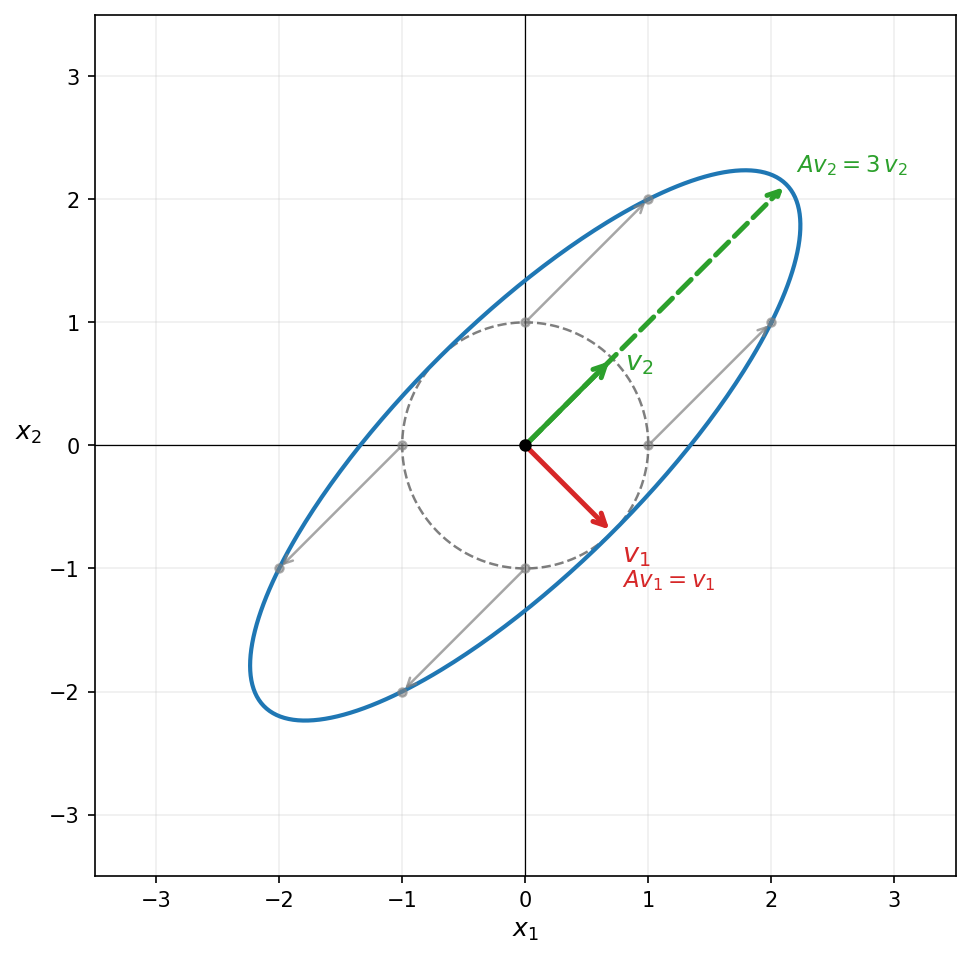
\includegraphics[width=0.62\textwidth]{figures/fig07_eigenvalues.png}
  \caption{Eigenvalues of $A = \bigl[\begin{smallmatrix}2&1\\1&2\end{smallmatrix}\bigr]$
    via the unit-circle picture.
    The dashed circle maps to the blue ellipse under $A$.
    Grey arrows connect a unit vector to its image.
    Red: $v_1$ with $Av_1 = v_1$ ($\lambda_1=1$, unchanged).
    Green solid/dashed: $v_2$ and $Av_2 = 3v_2$ ($\lambda_2=3$, tripled).
    Eigenvectors are exactly the directions that are only scaled, not rotated or sheared.}
\end{figure}

\begin{proposition}[Eigenvalue $\Leftrightarrow$ non-invertible shift]
  $\lambda$ is an eigenvalue of $L$ if and only if
  $\ker(L - \lambda I) \neq \{0\}$, i.e.\ $L - \lambda I$ is \textbf{not}
  invertible.
\end{proposition}
\begin{proof}
  $L(v) = \lambda v \Leftrightarrow (L - \lambda I)(v) = 0 \Leftrightarrow
  v \in \ker(L-\lambda I)$.
  Since $v \neq 0$, the kernel is non-trivial.
  By the Im-Ker Theorem, $L - \lambda I$ is then not injective, hence
  not invertible (for finite-dimensional $V$).
\end{proof}

\begin{remark}[Forward: eigenvectors give diagonalisation]
  If $L$ has $n$ linearly independent eigenvectors $v_1,\ldots,v_n$ with
  eigenvalues $\lambda_1,\ldots,\lambda_n$, then setting $P=[v_1|\cdots|v_n]$:
  \[
    P^{-1}AP = \operatorname{diag}(\lambda_1,\ldots,\lambda_n).
  \]
  Eigenvectors are exactly the basis that answers the simplification question.
  When such a basis exists, $L$ is called \emph{diagonalisable}.
\end{remark}

\subsection*{Python: eigenvalues and eigenvectors}
\begin{lstlisting}
import numpy as np

A = np.array([[1., 2.],
              [0., 3.]])
vals, vecs = np.linalg.eig(A)
print("eigenvalues:", vals)           # [1. 3.]
print("eigenvectors:\n", vecs)        # columns (normalised by numpy)

# Verify Av = lambda v for each eigenvector
for i in range(len(vals)):
    v = vecs[:, i]
    print(f"Av{i+1} = lam*v{i+1}:", np.allclose(A @ v, vals[i] * v))  # True

# Diagonalisation: P^{-1}AP = diag(lambda_1, lambda_2)
P   = vecs
D   = np.linalg.inv(P) @ A @ P
print("P^{-1}AP:\n", D.round(10))    # diagonal with [1, 3]
\end{lstlisting}

% ----- Page 36 -------------------------------------------------------
\subsection*{Building toward diagonalisation}

Since $v \neq 0$, we can complete it to a basis
$B = \{v, u_2, \ldots, u_n\}$.  The matrix of $L$ in basis $B$ is
formed by columns $[L]_B = [L(u_1) \mid L(u_2) \mid \cdots \mid L(u_n)]$.
Since $L(v) = \lambda v$ (i.e.\ $L(u_1) = \lambda_1 u_1$ in $B$-coordinates),
the first column is $\lambda_1 e_1$:
\[
  [L]_B =
  \begin{pmatrix}
    \lambda_1 & * & \cdots & * \\
    0         &   &        &   \\
    \vdots    &   & *      &   \\
    0         &   &        &
  \end{pmatrix}.
\]
If $u_2$ is also an eigenvector with $L(u_2) = \lambda_2 u_2$, $\lambda_2 \neq \lambda_1$,
the matrix simplifies further:
\[
  [L]_B =
  \begin{pmatrix}
    \lambda_1 & 0         & * & \cdots \\
    0         & \lambda_2 & * & \cdots \\
    0         & 0         &   &        \\
    \vdots    &           &   & *
  \end{pmatrix}.
\]
Continuing: if all $n$ basis vectors are eigenvectors, $[L]_B$ is diagonal.

\begin{remark}[Invariant subspaces]
  The zero pattern (zeros below each diagonal eigenvalue) reflects that
  $L$ maps $\operatorname{span}\{u_1,\ldots,u_k\}$ into itself for each $k$
  --- these are \emph{invariant subspaces} of $L$.  This concept will
  reappear in the Jordan normal form and SVD.
\end{remark}

\begin{proposition}[4.2.1]
  If $L(u_1) = \lambda_1 u_1$ and $L(u_2) = \lambda_2 u_2$ with
  $\lambda_1 \neq \lambda_2$, then $u_1$ and $u_2$ are linearly independent.
\end{proposition}
\begin{proof}
  Suppose $c_1 u_1 + c_2 u_2 = 0$.  Apply $L$:
  $\lambda_1 c_1 u_1 + \lambda_2 c_2 u_2 = 0$.
  Subtract $\lambda_1$ times the first equation:
  $(\lambda_2 - \lambda_1)c_2 u_2 = 0$.
  Since $u_2 \neq 0$ and $\lambda_1 \neq \lambda_2$, we get $c_2 = 0$,
  then $c_1 = 0$.
\end{proof}

\begin{corollary}
  Eigenvectors with pairwise distinct eigenvalues are linearly independent.
  Hence any $A \in \mathbb{R}^{n\times n}$ with $n$ distinct eigenvalues
  is automatically diagonalisable.
\end{corollary}

\medskip\noindent
The corollary says: as long as we keep finding eigenvectors with distinct
eigenvalues, we accumulate linearly independent vectors.  What is the
structure of $[L]_B$ when we have $k$ such eigenvectors but cannot (yet)
fill out the remaining $r = n - k$ slots with eigenvectors?

\begin{proposition}[Partial diagonalisation]\label{prop:partial-diag}
  Let $\dim V = n$.  Suppose $u_1,\ldots,u_k$ are eigenvectors of $L$
  with pairwise distinct eigenvalues $\lambda_1,\ldots,\lambda_k$.
  Extend to a basis
  \[
    B = \{u_1,\ldots,u_k,\; v_1,\ldots,v_r\}, \quad k + r = n.
  \]
  Then, in the basis $B$,
  \[
    [L]_B =
    \begin{pmatrix}
      \lambda_1 &        &           & * & \cdots & * \\
                & \ddots &           & \vdots & & \vdots \\
                &        & \lambda_k & * & \cdots & * \\
      0 & \cdots & 0         &   &        &   \\
      \vdots & & \vdots   &   & *      &   \\
      0 & \cdots & 0         &   &        &
    \end{pmatrix}
    =
    \begin{pmatrix} \Lambda & * \\ 0 & * \end{pmatrix},
  \]
  where $\Lambda = \operatorname{diag}(\lambda_1,\ldots,\lambda_k)$,
  the lower-left $r\times k$ block is zero, and the right-hand $*$ blocks
  are unconstrained.
\end{proposition}
\begin{proof}
  For each $i \le k$: in $B$-coordinates,
  $L(u_i) = \lambda_i u_i$ means the $i$-th column of $[L]_B$ is
  $\lambda_i e_i$ (eigenvalue in position $i$, zeros elsewhere).
  In particular all entries below row $k$ in those columns are zero.
  The columns corresponding to $v_1,\ldots,v_r$ are unconstrained
  (we imposed no condition on the $v_j$).
\end{proof}

\begin{remark}[Three cases by the value of $k$]
  \leavevmode
  \begin{itemize}
    \item $k = n$: every basis vector is an eigenvector,
          $[L]_B = \Lambda$ is diagonal --- $L$ is \emph{diagonalisable}.
    \item $k < n$: the lower-right $r\times r$ block $*$ captures
          the ``non-diagonalisable part''.  Understanding this block
          leads to the \emph{Jordan normal form}.
    \item $k = 0$: no eigenvectors at all over $\mathbb{R}$
          (e.g.\ a rotation in $\mathbb{R}^2$) --- must work over
          $\mathbb{C}$ to find them.
  \end{itemize}
\end{remark}

\subsection*{Python: partial diagonalisation and block structure}
\begin{lstlisting}
import numpy as np

# Matrix with only k=2 linearly independent eigenvectors out of n=3
# (repeated eigenvalue lambda=2 with 1-dim eigenspace)
A = np.array([[2., 1., 0.],
              [0., 2., 0.],
              [0., 0., 3.]], float)   # Jordan block in upper-left

vals, vecs = np.linalg.eig(A)
print("eigenvalues:", vals)           # [2. 2. 3.]
print("rank of eigenvector matrix:", np.linalg.matrix_rank(vecs))  # 2 < 3

# Distinct-eigenvalue case: partial diagonalisation is exact diagonalisation
B = np.array([[2., 1., 3.],
              [0., 4., 2.],
              [0., 0., 6.]], float)
vals2, vecs2 = np.linalg.eig(B)
D = np.linalg.inv(vecs2) @ B @ vecs2
print("P^{-1}AP (should be diagonal):\n", D.round(8))

# Verify zero pattern: lower-left block is 0
print("lower-left entries near zero:", np.allclose(D[1:, 0], 0))  # True
\end{lstlisting}

% ---- page 39: open questions ----
\subsection*{Open questions}

Three questions drive the rest of the course:

\begin{enumerate}
  \item \textbf{Which other matrices are diagonalizable?}
    Distinct eigenvalues are \emph{sufficient} but not necessary.
    The obstruction lives in the $r\times r$ block of the partial
    diagonalisation (Prop.~\ref{prop:partial-diag}): a matrix is
    diagonalizable iff that block can itself be diagonalized, i.e.\
    iff $V$ has a basis of eigenvectors.  Key positive answer:
    \emph{symmetric} (or, in general, \emph{normal}) matrices are
    always diagonalizable --- the spectral theorem, coming next.

  \item \textbf{How do we find eigenvalues and eigenvectors?}
    Theoretically: solve $\det(A - \lambda I) = 0$ for $\lambda$, then
    find $\ker(A - \lambda I)$ for each $\lambda$.  In practice: for
    $n \ge 5$ this is numerically unstable and wasteful; eigenvalues are
    computed via iterative algorithms (QR iteration), not by expanding a
    determinant.

  \item \textbf{Can we guarantee their existence?}
    Over $\mathbb{C}$: yes --- the Fundamental Theorem of Algebra says
    $\det(A - \lambda I) = 0$ always has $n$ roots (counted with
    multiplicity), so every matrix has at least one complex eigenvalue.
    Over $\mathbb{R}$: not in general --- a rotation by $90°$ in
    $\mathbb{R}^2$ has no real eigenvalues.  The guarantee is restored
    for symmetric matrices: all eigenvalues are real (proved via PSD,
    next section).
\end{enumerate}

\medskip\noindent
\textbf{Transition.}  Symmetric matrices $A = A^T$ form the class where
all three questions have clean answers: they are always diagonalizable,
their eigenvalues are always real, and there is a basis of orthonormal
eigenvectors.  This is the \emph{spectral theorem}, and it follows from
the theory of positive semidefinite matrices.

% ---- page 38 ----

\medskip\noindent
Putting it all together: if $L\colon V\to V$ has $n = \dim V$ distinct
eigenvalues $\lambda_1,\ldots,\lambda_n$ with eigenvectors $u_1,\ldots,u_n$,
then $B = \{u_1,\ldots,u_n\}$ is a basis (by Corollary above) and
\[
  [L]_B = \operatorname{diag}(\lambda_1,\lambda_2,\ldots,\lambda_n).
\]
The structure of $L$ in the eigenbasis $B$ is maximally simple, compared
with the standard-basis matrix $[L]_I = A$, which is generically dense.

\begin{definition}[Diagonalizable matrix]
  A matrix $A\in\mathbb{R}^{n\times n}$ is \emph{diagonalizable} if there
  exists an invertible $P\in\mathbb{R}^{n\times n}$ such that
  \[
    P^{-1}AP = \operatorname{diag}(\mu_1,\ldots,\mu_n).
  \]
  \textbf{Note:} the $\mu_i$ need \emph{not} be distinct.
  (Example: $A = I$ is diagonalized by any invertible $P$, with all
  $\mu_i = 1$.)
\end{definition}

\begin{remark}[Convention: $P^{-1}AP$ vs $PAP^{-1}$]
  Both conventions appear in the literature.  Our \S4.1 formula
  $A' = P^{-1}AP$ (columns of $P$ are the new basis vectors expressed in
  the old basis) is the one we use throughout.  If $P$ is the matrix whose
  $i$-th column is eigenvector $u_i$, then $P^{-1}AP = \Lambda$ —
  consistent with the change-of-basis formula.
\end{remark}

\begin{proposition}[4.2.2]
  If $A\in\mathbb{R}^{n\times n}$ has $n$ distinct eigenvalues
  $\lambda_1,\ldots,\lambda_n$ ($\lambda_i\neq\lambda_j$ for $i\neq j$),
  then $A$ is diagonalizable:
  \[
    P^{-1}AP = \operatorname{diag}(\lambda_1,\ldots,\lambda_n),
  \]
  where $P = [u_1 \mid \cdots \mid u_n]$ is the matrix of eigenvectors.
\end{proposition}
\begin{proof}
  By Corollary to Prop.\ 4.2.1, the $n$ eigenvectors are linearly
  independent, hence form a basis $B$.  In that basis $[L]_B$ is diagonal
  (Prop.~\ref{prop:partial-diag} with $k=n$, $r=0$).  The change-of-basis
  formula gives $[L]_B = P^{-1}AP = \Lambda$.
\end{proof}

\begin{definition}[Similar matrices]
  Two matrices $A, A'\in\mathbb{R}^{n\times n}$ are \emph{similar}
  (written $A'\sim A$) if $A' = P^{-1}AP$ for some invertible $P$.
  Similarity is an equivalence relation (reflexive, symmetric, transitive).
  Diagonalizable matrices are precisely those similar to a diagonal matrix.
\end{definition}

\begin{remark}[Finding eigenvalues in practice]
  The theoretical criterion $\ker(A-\lambda I)\neq\{0\}$ can be phrased as
  $\det(A-\lambda I) = 0$.  For small matrices ($n\le 4$) this gives a
  polynomial whose roots are the eigenvalues --- a clean formula.
  For $n\ge 5$ the Abel--Ruffini theorem says no closed-form root formula
  exists; for large $n$ computing the characteristic polynomial is
  numerically unstable and wasteful.  In practice, eigenvalues are found via
  iterative algorithms (QR iteration), not by expanding a determinant.
\end{remark}

\subsection*{Python: diagonalization}
\begin{lstlisting}
import numpy as np

# Diagonalization via eigenvectors
A = np.array([[1., 2.],
              [0., 3.]])
vals, P = np.linalg.eig(A)
Lambda = np.linalg.inv(P) @ A @ P
print("P^{-1}AP =\n", Lambda.round(10))   # diagonal: [1, 3]

# Similarity is an equivalence relation:
# A ~ A  (reflexive: P = I)
print("A ~ A:", np.allclose(np.linalg.inv(np.eye(2)) @ A @ np.eye(2), A))

# Eigenvalues are preserved under similarity
A2 = P @ np.diag([5., 7.]) @ np.linalg.inv(P)   # construct a similar matrix
print("eigenvalues of similar matrix:", np.linalg.eigvals(A2).round(8))  # [5, 7]
\end{lstlisting}

% ============================================================
\section{The Discrete Fourier Transform}
% ============================================================

\noindent
The DFT is the most important explicit diagonalisation in applied
mathematics.  It arises from a single observation: the cyclic shift
matrix $S$ has $N$ distinct eigenvalues, so it is diagonalisable, and
every matrix that commutes with $S$ is diagonalised by the same basis.

% ------------------------------------------------------------
\subsection*{The Shift Matrix}
% ------------------------------------------------------------

\noindent
Let $\omega = e^{2\pi i/N}$.  The \textbf{cyclic shift} on
$\mathbb{C}^N$ is $(Su)_j = u_{j+1\bmod N}$.  Its matrix is
$S_{jk}=\delta_{k,\,j+1\bmod N}$.  Since $S^N = I$, the minimal
polynomial of $S$ divides $x^N-1$, whose roots
$1,\omega,\omega^2,\ldots,\omega^{N-1}$ are distinct; hence $S$ is
diagonalisable with those eigenvalues.  A direct check shows the
corresponding unit eigenvectors are
\[
  v^{(k)}_j = \frac{1}{\sqrt{N}}\,\omega^{jk}, \qquad k=0,\ldots,N-1,
\]
and they are orthonormal: $\langle v^{(k)},v^{(\ell)}\rangle
= \frac{1}{N}\sum_j \omega^{j(k-\ell)} = \delta_{k\ell}$
(geometric series).

% ------------------------------------------------------------
\subsection*{Circulant Matrices and the Fourier Matrix}
% ------------------------------------------------------------

\begin{definition}
  $C\in M_N(\mathbb{C})$ is \textbf{circulant} with symbol $(c_0,\ldots,c_{N-1})$
  if $C_{jk}=c_{(j-k)\bmod N}$, i.e.\ each row is the previous one
  shifted right by one.  Equivalently, $C=\sum_{m=0}^{N-1}c_m S^m$.
\end{definition}

\noindent
The \textbf{Fourier matrix} $F=\frac{1}{\sqrt{N}}(\omega^{jk})_{j,k=0}^{N-1}$
is unitary ($F^*F=I$) and simultaneously diagonalises every circulant:

\begin{theorem}
  $F^*CF = \operatorname{diag}(\hat{c}_0,\ldots,\hat{c}_{N-1})$, where
  $\hat{c}_k = \sum_{j=0}^{N-1}c_j\,\omega^{jk}$ is the \textbf{DFT} of
  the symbol.
\end{theorem}
\begin{proof}
  $F^*CF = \sum_m c_m (F^*S^m F) = \sum_m c_m \Lambda_S^m$,
  where $\Lambda_S=\operatorname{diag}(1,\omega,\ldots,\omega^{N-1})$.
  The $(k,k)$ entry is $\sum_m c_m\omega^{mk}=\hat{c}_k$.
\end{proof}

\noindent
The DFT of $u\in\mathbb{C}^N$ is $\hat u_k = \sum_j u_j\omega^{-jk}$
with inverse $u_j = \frac{1}{N}\sum_k\hat u_k\omega^{jk}$.

% ------------------------------------------------------------
\subsection*{The Convolution Theorem and the FFT}
% ------------------------------------------------------------

\noindent
The \textbf{cyclic convolution} $(c*u)_j=\sum_m c_{(j-m)\bmod N}u_m$
is the circulant matrix-vector product $Cu$.
By the diagonalisation theorem:

\begin{theorem}[Convolution theorem]
  $\widehat{c*u}=\hat c\cdot\hat u$ (pointwise).
\end{theorem}
\begin{proof}
  $F^*(Cu)=F^*C(FF^*)u=(F^*CF)(F^*u)=\operatorname{diag}(\hat c)\cdot\hat u$.
\end{proof}

\noindent
This reduces cyclic convolution from $O(N^2)$ to $O(N\log N)$ once
the DFT is computed efficiently.  The \textbf{Cooley--Tukey FFT}
achieves this by splitting $u$ into even- and odd-indexed halves:
\[
  \hat u_k = \hat u^{(e)}_k + \omega^{-k}\hat u^{(o)}_k, \qquad
  \hat u_{k+N/2} = \hat u^{(e)}_k - \omega^{-k}\hat u^{(o)}_k,
\]
reducing the $N$-point DFT to two $N/2$-point DFTs.  The recurrence
$T(N)=2T(N/2)+O(N)$ solves to $T(N)=O(N\log N)$.

% ------------------------------------------------------------
\subsection*{Python: DFT, FFT, and the Convolution Theorem}
% ------------------------------------------------------------

\begin{lstlisting}
import numpy as np

N = 128
np.random.seed(0)
u = np.random.randn(N)
u_hat = np.fft.fft(u)

# Unitarity: ||u||^2 = (1/N)||u_hat||^2  (Parseval)
print("Parseval error:", abs(np.dot(u, u) - np.dot(u_hat, u_hat.conj()).real / N))

# Shift theorem: fft(roll(u,1))[k] = omega^k * u_hat[k]
omega = np.exp(2j * np.pi * np.arange(N) / N)
shift_err = np.max(np.abs(np.fft.fft(np.roll(u, 1)) - omega * u_hat))
print("Shift theorem error:", shift_err)

# Convolution theorem: circulant matrix-vector product via FFT
c = np.zeros(N); c[:4] = 0.25           # 4-tap box filter
C = np.array([[c[(j-k)%N] for k in range(N)] for j in range(N)])
conv_direct = C @ u
conv_fft    = np.real(np.fft.ifft(np.fft.fft(c) * u_hat))
print("Convolution error:", np.max(np.abs(conv_direct - conv_fft)))
\end{lstlisting}

% ------------------------------------------------------------
\subsection*{2D DFT and the Lecture~1 Transfer Rule}
% ------------------------------------------------------------

\noindent
The 2D DFT on $\mathbb{Z}_N^2$ is separable (apply 1D FFT to rows,
then columns) at cost $O(N^2\log N)$.  Any
\textbf{translation-invariant} operator $(Tu)_{m,n}=\sum_{a,b}h_{a,b}\,u_{m-a,n-b}$
is diagonalised by the 2D plane waves $e^{2\pi i(k_1 m+k_2 n)/N}$
with eigenvalue $\hat h_{k_1,k_2}$ (the 2D DFT of the kernel).

\begin{example}[Lecture~1 transfer rule]
  The rule $u_{m,n}(t+1)=p\,u_{m+1,n+1}(t)+q\,u_{m-1,n-1}(t)$ has kernel
  $h_{a,b}=p\,\delta_{a,-1}\delta_{b,-1}+q\,\delta_{a,1}\delta_{b,1}$
  with transfer function
  \[
    \hat h_{k_1,k_2}=p\,e^{i(\kappa_1+\kappa_2)}+q\,e^{-i(\kappa_1+\kappa_2)},
    \qquad \kappa_j=2\pi k_j/N.
  \]
  This depends only on $\kappa_1+\kappa_2$, which is exactly why the
  anti-diagonal direction ($\kappa_1=-\kappa_2$) gives a
  \emph{constant} $|\hat h|=p+q$ for all modes: those modes all see
  the same kernel value.  The amplification map in Lecture~1 is just
  the modulus of the 2D DFT of the kernel.  The spectrum
  $\{pe^{i\theta}+qe^{-i\theta}:\theta\in[0,2\pi)\}$ is an ellipse in
  $\mathbb{C}$ with semi-axes $p+q$ and $|p-q|$.
\end{example}

\begin{lstlisting}
import numpy as np

N, p, q = 256, 1.2, 0.8
h = np.zeros((N, N))
h[-1, -1] = p; h[1, 1] = q          # kernel (periodic indexing)
H = np.fft.fft2(h)
print(f"max |H| = {np.max(np.abs(H)):.6f}  (should be p+q = {p+q})")
print(f"min |H| = {np.min(np.abs(H)):.6f}  (should be |p-q| = {abs(p-q)})")

def step(u): return p*np.roll(np.roll(u,-1,0),-1,1)+q*np.roll(np.roll(u,1,0),1,1)
u0 = np.random.randn(N, N)*0.01
u_sim = u0.copy()
for _ in range(30): u_sim = step(u_sim)
u_fft = np.real(np.fft.ifft2(np.fft.fft2(u0) * H**30))
print(f"Prediction error at t=30: {np.max(np.abs(u_sim - u_fft)):.2e}")
\end{lstlisting}

% ============================================================
\section{Positive Semidefinite Matrices (\S4.3)}
% ============================================================
% Pages 40--

\subsection*{Definition and first properties}

\begin{definition}[PSD via factorization]
  A matrix $A\in\mathbb{R}^{n\times n}$ is called \emph{positive semidefinite}
  (PSD) if
  \[
    A = B^T B \quad \text{for some } B\in\mathbb{R}^{m\times n}.
  \]
  It is \emph{positive definite} (PD) if additionally $\ker B = \{0\}$.
\end{definition}

\begin{remark}[Two common definitions --- not always equivalent]
  Several definitions of PSD appear in the literature:
  \begin{enumerate}
    \item \textbf{(Our definition)} $A = B^T B$ for some $B$.
    \item \textbf{(Quadratic form)} $\forall x\in\mathbb{R}^n,\ x^TAx\ge 0$.
      This does \emph{not} require $A$ to be symmetric.
    \item \textbf{(Symmetric + quadratic form)} $A = A^T$ and $x^TAx\ge 0$
      for all $x$.
  \end{enumerate}
  Our definition (1) automatically gives $A^T = (B^TB)^T = B^TB = A$, so it
  implies symmetry.  Definitions (1) and (3) are equivalent for symmetric
  matrices; definition (2) is strictly weaker.  Throughout these notes we use
  definition (1)/(3): PSD means symmetric with $x^TAx\ge 0$.
\end{remark}

\noindent
\textbf{Quadratic forms.}  The expression $f(x) = x^TAx$ is called a
\emph{quadratic form}.  For a PSD matrix $A = B^TB$:
\[
  f(x) = x^T B^T B x = (Bx)^T(Bx) = \|Bx\|^2 \ge 0,
\]
using the $\ell^2$-norm $\|y\|^2 = y_1^2 + \cdots + y_m^2$.
So $f(x) \ge 0$ with minimum $f(x) = 0$ achieved precisely on $\ker B$.

\medskip\noindent
\textbf{Key example.} $A^TA$ is always PSD: take $B = A$, then
$A^TA = B^TB$.  This is the matrix in the normal equations.

\subsection*{Kernel of a PSD matrix}

\begin{proposition}
  If $A = B^TB$, then $\ker B = \ker A$.
\end{proposition}
\begin{proof}
  This is the same argument as in \S3 (normal equations): $Ax = 0$ iff
  $x^TAx = 0$ iff $\|Bx\|^2 = 0$ iff $Bx = 0$.
  More explicitly: $\ker B \subseteq \ker A$ is clear ($Bx=0\Rightarrow
  B^TBx=0$).  Conversely, $Ax = B^TBx = 0$ implies $x^TB^TBx = \|Bx\|^2 = 0$,
  so $Bx = 0$.
\end{proof}

\noindent
\textbf{Consequence.} Let $V = \mathbb{R}^n = \ker A \oplus (\ker A)^\perp$.
On $(\ker A)^\perp$, we have $f(x) = \|Bx\|^2 = 0 \Rightarrow x = 0$, so
$A$ is \emph{positive definite on $(\ker A)^\perp$}.

\subsection*{Python: three equivalent characterizations}
\begin{lstlisting}
import numpy as np

rng = np.random.default_rng(42)
B = rng.standard_normal((4, 3))     # tall matrix
A = B.T @ B                         # 3x3 PSD by construction

# (1) Check symmetry
print("symmetric:", np.allclose(A, A.T))

# (2) Check all eigenvalues >= 0
vals = np.linalg.eigvalsh(A)        # eigvalsh: symmetric matrix
print("eigenvalues:", vals.round(8))        # all >= 0

# (3) Check x^T A x >= 0 for random x
xs = rng.standard_normal((1000, 3))
quad_forms = np.einsum('ni,ij,nj->n', xs, A, xs)
print("all x^TAx >= 0:", np.all(quad_forms >= -1e-12))

# (4) ker B = ker A
from scipy.linalg import null_space
print("null_space(B) approx empty (full rank B):", null_space(B).shape[1])
\end{lstlisting}

% ---- page 41 ----

\subsection*{Invariant subspaces and restrictions}

\begin{definition}[Invariant subspace]
  A subspace $U \le V$ is \emph{invariant under} $L \in \mathcal{L}(V,V)$
  (or \emph{$L$-invariant}) if $L(U) \subseteq U$, i.e.\
  $L(u) \in U$ for every $u \in U$.
\end{definition}

\begin{example}
  $\ker A$ is always $A$-invariant: if $Au = 0$ then $A(Au) = A \cdot 0 = 0$,
  so $Au \in \ker A$.
\end{example}

\begin{definition}[Restriction]
  If $U \le V$ is $L$-invariant, the \emph{restriction} $L\big|_U \in
  \mathcal{L}(U, U)$ is defined by
  \[
    L\big|_U(u) = L(u) \quad \forall\, u \in U.
  \]
  The restriction is well-defined precisely because $U$ is invariant.
\end{definition}

\subsection*{Symmetric matrices preserve orthogonal complements}

\begin{lemma}\label{lem:perp-invariant}
  Let $A \in \mathbb{R}^{n\times n}$ be symmetric ($A^T = A$) and let
  $U \le \mathbb{R}^n$ be $A$-invariant.  Then $U^\perp$ is also $A$-invariant.
\end{lemma}
\begin{proof}
  Take $w \in U^\perp$, so $\langle w, u\rangle = 0$ for all $u \in U$.
  We must show $Aw \in U^\perp$, i.e.\ $\langle Aw, u\rangle = 0$ for all
  $u \in U$:
  \[
    \langle Aw, u\rangle = (Aw)^T u = w^T A^T u = w^T A u.
  \]
  Since $U$ is $A$-invariant, $Au \in U$; since $w \in U^\perp$,
  $w^T(Au) = 0$.  Hence $\langle Aw, u\rangle = 0$, so $Aw \in U^\perp$.
\end{proof}

\begin{remark}[Inductive sketch of the spectral theorem]
  Lemma~\ref{lem:perp-invariant} is the engine of the spectral theorem.
  Let $A$ be symmetric and take any eigenvalue $\lambda$ with eigenvector $v$.
  Set $U = \operatorname{span}\{v\}$; this is $A$-invariant.  By the lemma,
  $U^\perp$ is also $A$-invariant, so $A\big|_{U^\perp}$ is a well-defined
  symmetric map on an $(n-1)$-dimensional space.  Apply the argument
  inductively: at each step peel off one eigenvalue and restrict to the
  orthogonal complement.  The result is an orthonormal basis of eigenvectors ---
  the spectral theorem.
\end{remark}

\subsection*{Python: $U^\perp$ invariance for a symmetric matrix}
\begin{lstlisting}
import numpy as np

# Build a symmetric matrix
rng = np.random.default_rng(0)
M = rng.standard_normal((4, 4))
A = M + M.T                          # symmetric

# Find an eigenspace (A-invariant subspace U)
vals, vecs = np.linalg.eigh(A)       # orthonormal eigenvectors
U = vecs[:, :2]                      # span of first two eigenvectors

# Orthogonal complement U_perp: span of remaining eigenvectors
U_perp = vecs[:, 2:]

# Check A maps U_perp into U_perp: project A @ w onto U and check it's ~0
for i in range(U_perp.shape[1]):
    w = U_perp[:, i]
    Aw = A @ w
    component_in_U = U @ (U.T @ Aw)  # projection of Aw onto U
    print(f"||proj_U(A w_{i})||: {np.linalg.norm(component_in_U):.2e}")
    # should be ~0 (machine precision)
\end{lstlisting}

% ---- page 42 ----

\subsection*{The spectral theorem: proof via constrained optimisation}

\textbf{Goal.}  We want to show that every symmetric $A\in\mathbb{R}^{n\times n}$
has a real eigenvector.  Combined with the inductive argument
(Lemma~\ref{lem:perp-invariant}), this gives an orthonormal eigenbasis ---
the spectral theorem.

\medskip\noindent
On $U^\perp = (\ker A)^\perp$ we have $f(x) = x^TAx > 0$ for all $x\ne 0$,
so the quadratic form is a ``bowl'' with global minimum $f(0) = 0$.
(Note: this holds on $U^\perp$ specifically, not on all of $\mathbb{R}^n$.)
Consider the constrained maximum:
\[
  \max_{\|x\|=1} f(x).
\]
The unit sphere $\{x : \|x\|=1\}$ is compact and $f$ is continuous,
so the maximum is attained at some $v$ with $\|v\|=1$.

\begin{proposition}[Maximizer is an eigenvector]
  Let $v\in\mathbb{R}^n$, $\|v\|=1$, satisfy
  $f(v) = \max_{\|x\|=1} f(x)$.
  Then $Av = \lambda v$ with $\lambda = f(v) \ge 0$.
\end{proposition}
\begin{proof}
  For any $w\in\langle v\rangle^\perp$, consider the unit-normalised path
  \[
    u(t) = \frac{v + tw}{\|v + tw\|}, \quad
    g(t) = f(u(t)) = \frac{(v+tw)^T A(v+tw)}{\|v+tw\|^2}.
  \]
  Since $w \perp v$ we have $\|v+tw\|^2 = \|v\|^2 + t^2\|w\|^2 = 1 + t^2\|w\|^2$, so
  \[
    g(t) = \frac{v^TAv + 2t\,w^TAv + t^2\,w^TAw}{1 + t^2\|w\|^2}.
  \]
  Since $v$ is a maximizer on the unit sphere, $g'(0) = 0$.

  \textbf{Exercise.}  Show using the quotient rule (and $w^Tv = 0$, $\|v\|=1$)
  that $g'(0) = 2w^TAv$.

  Hence $w^TAv = 0$ for all $w\in\langle v\rangle^\perp$, i.e.\
  $Av \perp w$ for every $w\perp v$.  This means
  $Av \in \langle v\rangle^{\perp\perp} = \langle v\rangle$,
  so $Av = \lambda v$ for some $\lambda\in\mathbb{R}$.
  Taking $w = v$: $\lambda = v^TAv = f(v) \ge 0$ (since $A$ is PSD).
\end{proof}

% ---- page 43 ----

\begin{corollary}[PSD $\Rightarrow$ eigenvalues $\ge 0$]
  If $A$ is PSD then every eigenvalue satisfies $\lambda \ge 0$.
\end{corollary}
\begin{proof}
  If $Av = \lambda v$, $v\ne 0$, then
  $\lambda \|v\|^2 = v^TAv \ge 0$, so $\lambda \ge 0$.
\end{proof}

\begin{theorem}[Spectral theorem]\label{thm:spectral}
  Let $A\in\mathbb{R}^{n\times n}$ be symmetric ($A = A^T$).  Then:
  \begin{enumerate}
    \item All eigenvalues of $A$ are real.
    \item $A$ has an orthonormal basis of eigenvectors:
          $A = Q\Lambda Q^T$ where $Q$ is orthogonal and
          $\Lambda = \operatorname{diag}(\lambda_1,\ldots,\lambda_n)$.
    \item If additionally $A$ is PSD, then $\lambda_i \ge 0$ for all $i$.
  \end{enumerate}
\end{theorem}
\begin{proof}[Proof (induction via Lemma~\ref{lem:perp-invariant})]
  The proposition gives a unit eigenvector $v_1$ with $\lambda_1 = f(v_1) \ge 0$
  (the largest eigenvalue).  Set $W = \langle v_1\rangle$; by
  Lemma~\ref{lem:perp-invariant}, $W^\perp$ is $A$-invariant and inherits
  symmetry.  Apply the proposition to $A\big|_{W^\perp}$, obtaining $v_2$
  with $v_2\perp v_1$.  Repeat $n$ times to produce an orthonormal eigenbasis
  $\{v_1,\ldots,v_n\}$.  Setting $Q = [v_1\mid\cdots\mid v_n]$ gives
  $AQ = Q\Lambda$, i.e.\ $A = Q\Lambda Q^T$.
\end{proof}

% ---- page 44 ----

\begin{definition}[Eigenspace]
  For $L\in\mathcal{L}(V,V)$ and $\lambda\in\mathbb{F}$, the
  \emph{$\lambda$-eigenspace} of $L$ is
  \[
    E_\lambda = \{v\in V : L(v) = \lambda v\} = \ker(L - \lambda\operatorname{id}).
  \]
  Note $E_\lambda \le V$.  The dimension $\dim E_\lambda$ is the
  \emph{geometric multiplicity} of $\lambda$.
\end{definition}

\begin{theorem}[4.3.1 — Spectral theorem for PSD matrices]
  Let $A\in\mathbb{R}^{n\times n}$ be PSD.  Then there exists an
  orthonormal eigenbasis $\{v_1,\ldots,v_n\}$ (i.e.\
  $v_i^Tv_j = \delta_{ij}$) such that $Av_i = \lambda_i v_i$,
  $\lambda_i \ge 0$.  Setting $P = [v_1\mid\cdots\mid v_n]$ (orthogonal,
  $P^TP = I$, $P^{-1} = P^T$):
  \[
    P^T A P = \operatorname{diag}(\lambda_1,\ldots,\lambda_n), \quad
    \lambda_i \ge 0.
  \]
\end{theorem}

\begin{figure}[h!]
  \centering
  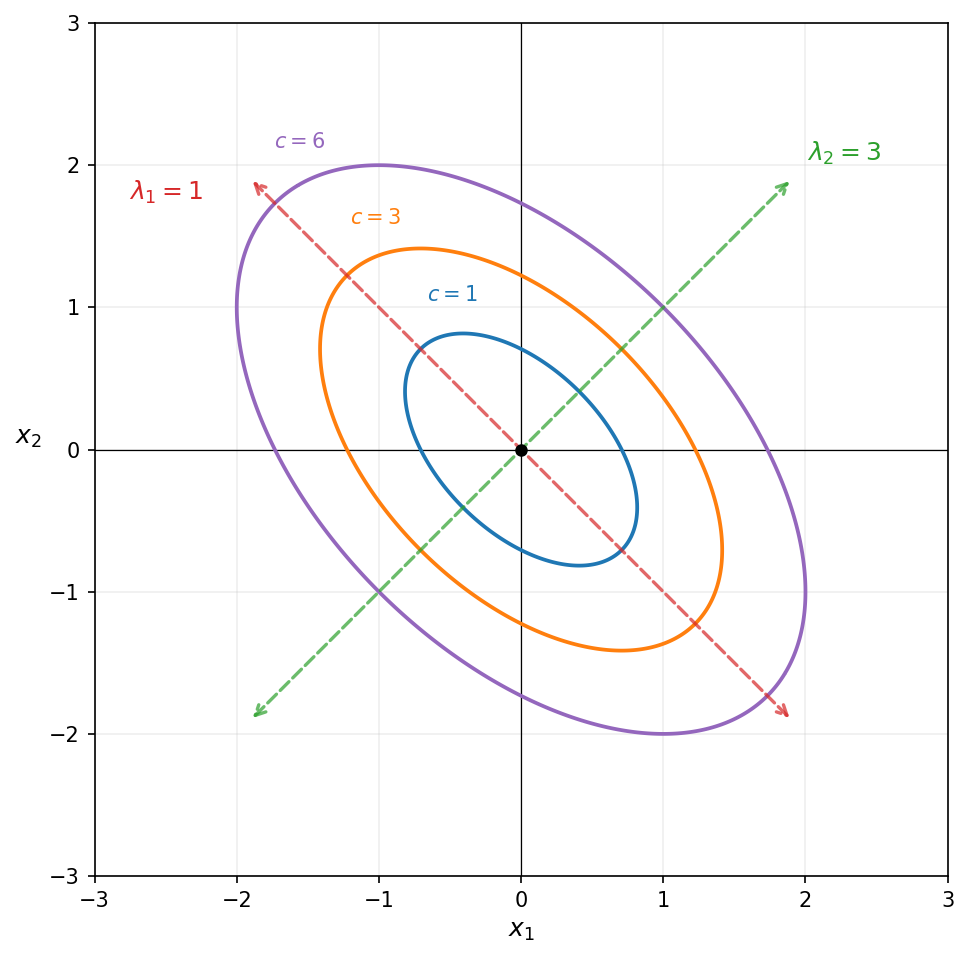
\includegraphics[width=0.62\textwidth]{figures/fig08_psd_quadratic.png}
  \caption{Level curves $x^T\!Ax = c$ for $A = \bigl[\begin{smallmatrix}2&1\\1&2\end{smallmatrix}\bigr]$,
    $c = 1, 3, 6$.
    The curves are ellipses whose principal axes align with the eigenvectors
    (dashed lines).
    The semi-axis length along eigenvector $v_i$ equals $\sqrt{c/\lambda_i}$,
    so the larger eigenvalue $\lambda_2 = 3$ corresponds to the \emph{shorter} axis.}
\end{figure}

\begin{remark}[$P^TAP$ vs $P^{-1}AP$]
  Because $P$ is orthogonal ($P^T = P^{-1}$), the change-of-basis formula
  $P^{-1}AP = \Lambda$ simplifies to $P^TAP = \Lambda$.  This is a strictly
  stronger form of diagonalizability: the eigenbasis is not only a basis but an
  \emph{orthonormal} one.  General diagonalizable matrices only have
  $P^{-1}AP = \Lambda$ with $P$ possibly non-orthogonal.
\end{remark}

\begin{remark}[Forward pointer: SVD]
  For a PSD matrix, the SVD coincides with the eigendecomposition:
  $A = Q\Lambda Q^T$ with $\Lambda = \Sigma^2$.  For a general rectangular
  matrix $A\in\mathbb{R}^{m\times n}$, the SVD $A = U\Sigma V^T$ replaces
  the eigendecomposition --- applying the spectral theorem to $A^TA$ and
  $AA^T$ simultaneously.  This is the subject of \S4.4.
\end{remark}

\subsection*{Python: largest eigenvector as constrained maximum}
\begin{lstlisting}
import numpy as np

rng = np.random.default_rng(7)
M = rng.standard_normal((4, 4))
A = M + M.T                          # symmetric 4x4

# True largest eigenvalue and eigenvector
vals, vecs = np.linalg.eigh(A)       # eigenvalues in ascending order
lambda_max = vals[-1]
v_max = vecs[:, -1]
print(f"lambda_max = {lambda_max:.6f},  f(v_max) = {v_max @ A @ v_max:.6f}")

# Sample random unit vectors and compute f(x) = x^T A x
N = 100_000
X = rng.standard_normal((N, 4))
X /= np.linalg.norm(X, axis=1, keepdims=True)   # project onto unit sphere
fvals = np.einsum('ni,ij,nj->n', X, A, X)

print(f"max f(x) over {N} samples: {fvals.max():.6f}")
print(f"ratio (should be close to 1): {fvals.max() / lambda_max:.6f}")

# ------------------------------------------------------------------
# Theorem 4.3.1: P^T A P = Lambda, P^T P = I  (PSD matrix)
B = rng.standard_normal((5, 4))
A_psd = B.T @ B                      # 4x4 PSD by construction
vals_psd, Q = np.linalg.eigh(A_psd)  # Q orthogonal, vals >= 0

print("\nSpectral theorem verification:")
print("eigenvalues (>= 0):", vals_psd.round(8))
print("P^T P = I:", np.allclose(Q.T @ Q, np.eye(4)))
Lambda = Q.T @ A_psd @ Q
print("P^T A P diagonal:", np.allclose(Lambda, np.diag(vals_psd)))
print("diagonal entries:", np.diag(Lambda).round(8))
\end{lstlisting}

% ============================================================
\section{Trace}
% ============================================================

\begin{definition}[Axiomatic characterization]
  The \emph{trace} is the unique linear map
  $\operatorname{tr}: \mathbb{F}^{n\times n}\to\mathbb{F}$ satisfying:
  \begin{enumerate}
    \item $\operatorname{tr}(AB) = \operatorname{tr}(BA)$ for all $A,B$.
    \item $\operatorname{tr}(I) = n$.
  \end{enumerate}
\end{definition}

\begin{proposition}
  $\operatorname{tr}(A) = \sum_i a_{ii}$ (sum of diagonal entries).
\end{proposition}
\begin{proof}
  Let $E_{ij}$ be the standard matrix units.  By linearity, it suffices to
  compute $\operatorname{tr}(E_{ij})$.  If $i\ne j$:
  $\operatorname{tr}(E_{ij}) = \operatorname{tr}(E_{ii}E_{ij}) =
  \operatorname{tr}(E_{ij}E_{ii}) = 0$.
  For $i=j$: for any $i,j$ there is a permutation matrix $P$ with
  $P^{-1}E_{jj}P = E_{ii}$.  By cyclicity,
  $\operatorname{tr}(E_{ii}) = \operatorname{tr}(P^{-1}E_{jj}P) = \operatorname{tr}(E_{jj})$.
  So all $\operatorname{tr}(E_{ii})$ are equal; since $I = \sum_i E_{ii}$ and
  $\operatorname{tr}(I) = n$, we get $\operatorname{tr}(E_{ii}) = 1$.
  Hence $\operatorname{tr}(A) = \sum_i a_{ii}$.
\end{proof}

\begin{proposition}[Similarity invariance]
  $\operatorname{tr}(P^{-1}AP) = \operatorname{tr}(A)$.
\end{proposition}
\begin{proof}
  $\operatorname{tr}(P^{-1}AP) = \operatorname{tr}(APP^{-1}) = \operatorname{tr}(A)$.
\end{proof}

\begin{corollary}
  If $A$ is diagonalizable with eigenvalues $\lambda_1,\ldots,\lambda_n$, then
  $\operatorname{tr}(A) = \sum_i \lambda_i$.
\end{corollary}

% ============================================================
\section{Singular Value Decomposition (\S4.4)}
% ============================================================

\subsection*{Motivation: symmetric is not enough}

The spectral theorem (Thm.~\ref{thm:spectral}) gives a complete
orthonormal eigenbasis for \emph{symmetric} matrices.  Most matrices in
practice --- data matrices, regression matrices, image matrices --- are
rectangular and not symmetric.  The SVD extends the spectral theorem to
every $A\in\mathbb{R}^{m\times n}$.

\subsection*{Step 1: $A^TA$ is PSD}

\begin{lemma}
  For any $A\in\mathbb{R}^{m\times n}$, the matrices $A^TA\in\mathbb{R}^{n\times n}$
  and $AA^T\in\mathbb{R}^{m\times m}$ are both symmetric PSD.
\end{lemma}
\begin{proof}
  $(A^TA)^T = A^T(A^T)^T = A^TA$, so symmetric.
  $x^T(A^TA)x = (Ax)^T(Ax) = \|Ax\|^2 \ge 0$, so PSD.
  Identical argument for $AA^T$.
\end{proof}

\noindent
By the spectral theorem, $A^TA$ has an orthonormal eigenbasis
$\{v_1,\ldots,v_n\}$ with eigenvalues $\lambda_1 \ge \cdots \ge \lambda_n \ge 0$.

\subsection*{Step 2: right singular vectors and singular values}

Write $A^TAv_i = \lambda_i v_i$.  Define the \emph{singular values}
\[
  \sigma_i = \sqrt{\lambda_i} \ge 0, \qquad i = 1,\ldots,n.
\]
Let $r = \operatorname{rank}(A)$.  Then $\sigma_1 \ge \cdots \ge \sigma_r > 0 =
\sigma_{r+1} = \cdots = \sigma_n$ (since $\ker(A^TA) = \ker A$ by \S4.3,
so $\lambda_i = 0 \Leftrightarrow v_i \in \ker A$).

The $v_i$ are the \emph{right singular vectors} of $A$.

\subsection*{Step 3: left singular vectors}

\begin{lemma}
  For $i \le r$, define $u_i = Av_i / \sigma_i$.  Then:
  \begin{enumerate}
    \item $u_i$ is a unit vector: $\|u_i\| = 1$.
    \item $u_i \perp u_j$ for $i \ne j$.
    \item $AA^T u_i = \sigma_i^2\, u_i$ (so $u_i$ is an eigenvector of $AA^T$).
  \end{enumerate}
\end{lemma}
\begin{proof}
  (1): $\|u_i\|^2 = \|Av_i\|^2/\sigma_i^2 = v_i^T A^TAv_i/\sigma_i^2
  = \sigma_i^2/\sigma_i^2 = 1$.

  (2): $\langle u_i, u_j\rangle = (Av_i)^T(Av_j)/(\sigma_i\sigma_j)
  = v_i^T A^T A v_j / (\sigma_i\sigma_j)
  = \sigma_j^2 v_i^T v_j / (\sigma_i\sigma_j) = 0$ (since $v_i\perp v_j$).

  (3): $AA^T u_i = AA^T(Av_i/\sigma_i) = A(A^TAv_i)/\sigma_i
  = A(\sigma_i^2 v_i)/\sigma_i = \sigma_i\, Av_i = \sigma_i^2 u_i$.
\end{proof}

Extend $\{u_1,\ldots,u_r\}$ to a full orthonormal basis $\{u_1,\ldots,u_m\}$
of $\mathbb{R}^m$ (the remaining $u_{r+1},\ldots,u_m$ span $\ker(A^T)$).
These are the \emph{left singular vectors}.

\subsection*{Step 4: assembling the SVD}

Set
\[
  U = [u_1\mid\cdots\mid u_m]\in\mathbb{R}^{m\times m}, \quad
  V = [v_1\mid\cdots\mid v_n]\in\mathbb{R}^{n\times n}, \quad
  \Sigma\in\mathbb{R}^{m\times n}\ (\text{``diagonal'': }\Sigma_{ii}=\sigma_i).
\]

\begin{theorem}[Singular Value Decomposition]\label{thm:svd}
  For any $A\in\mathbb{R}^{m\times n}$ with $\operatorname{rank}(A)=r$,
  \[
    A = U\Sigma V^T,
  \]
  where $U\in\mathbb{R}^{m\times m}$ and $V\in\mathbb{R}^{n\times n}$ are
  orthogonal, and $\Sigma\in\mathbb{R}^{m\times n}$ has
  $\sigma_1\ge\cdots\ge\sigma_r>0$ on its main diagonal and zeros elsewhere.
\end{theorem}
\begin{proof}
  Check column by column.  For $i \le r$:
  $(U\Sigma V^T)v_i = U(\Sigma e_i) = \sigma_i\,U e_i = \sigma_i u_i = Av_i$.
  For $i > r$: $Av_i = 0$ (since $v_i\in\ker A$), and
  $(U\Sigma V^T)v_i = \sigma_i u_i = 0$.
  Since $\{v_i\}$ is a basis of $\mathbb{R}^n$, $A = U\Sigma V^T$.
\end{proof}

\begin{remark}[Four fundamental subspaces via SVD]
  The SVD makes the four subspaces explicit:
  \begin{align*}
    \operatorname{col}(A)   &= \operatorname{span}\{u_1,\ldots,u_r\}, \\
    \ker(A^T)               &= \operatorname{span}\{u_{r+1},\ldots,u_m\}, \\
    \operatorname{row}(A)   &= \operatorname{span}\{v_1,\ldots,v_r\}, \\
    \ker(A)                 &= \operatorname{span}\{v_{r+1},\ldots,v_n\}.
  \end{align*}
\end{remark}

\begin{remark}[Geometric picture]
  $A$ factors as three simple operations:
  \[
    \mathbb{R}^n
    \xrightarrow{V^T} \text{rotate}
    \xrightarrow{\Sigma} \text{stretch (axis $i$ by $\sigma_i$)}
    \xrightarrow{U} \text{rotate}
    \in \mathbb{R}^m.
  \]
  The image of the unit sphere under $A$ is an ellipsoid with semi-axis
  lengths $\sigma_1\ge\cdots\ge\sigma_r$ along directions $u_1,\ldots,u_r$.
\end{remark}

\begin{figure}[h!]
  \centering
  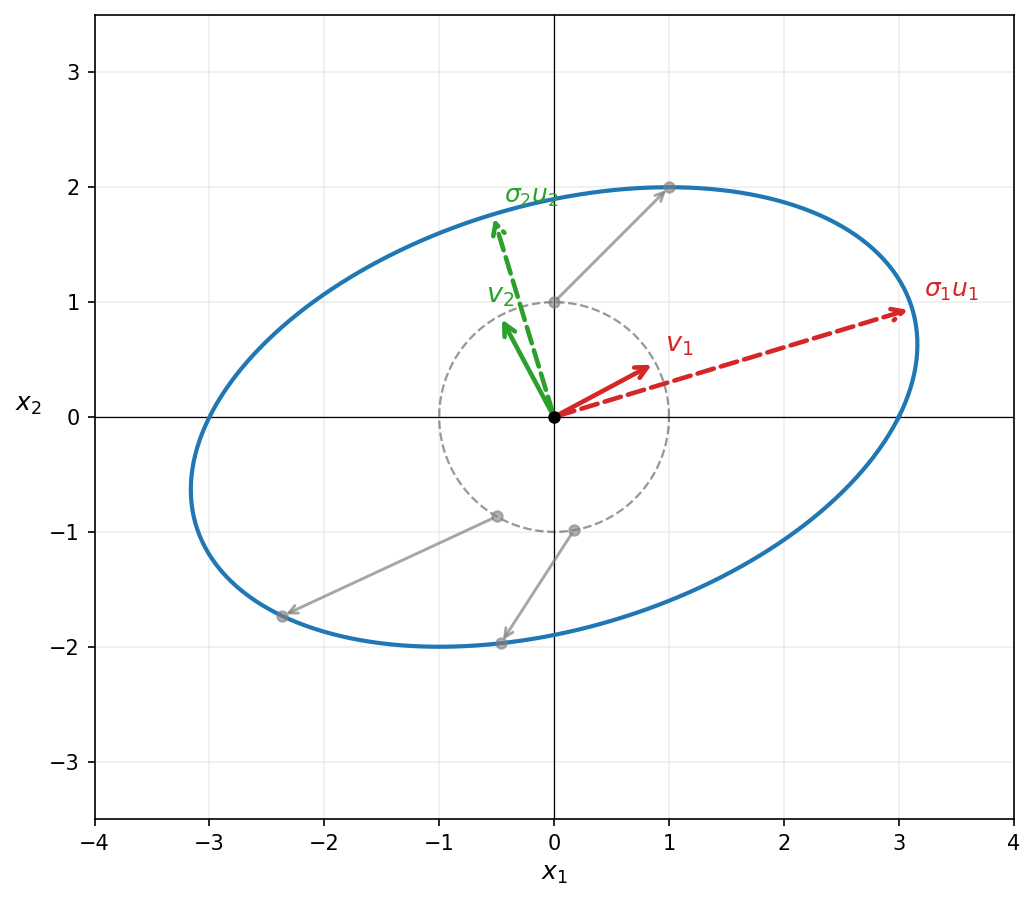
\includegraphics[width=0.62\textwidth]{figures/fig09_svd_geometry.png}
  \caption{SVD geometry for $A = \bigl[\begin{smallmatrix}3&1\\0&2\end{smallmatrix}\bigr]$.
    The dashed unit circle maps to the blue ellipse.
    Solid arrows: right singular vectors $v_1, v_2$ (input directions).
    Dashed arrows: $\sigma_i u_i$ (output directions, scaled by singular values).
    Because $A$ is not symmetric, input and output directions differ ---
    grey arrows show the rotation and stretching for three sample unit vectors.}
\end{figure}

% ============================================================
% ============================================================
\subsection*{Low-rank approximation and the Eckart--Young theorem}
% ============================================================

\subsubsection*{Outer-product expansion}

Writing $U\Sigma V^T$ column by column gives the \emph{outer-product form}:
\[
  A = \sum_{i=1}^r \sigma_i\, u_i v_i^T.
\]
Each term $\sigma_i u_i v_i^T$ is a rank-1 matrix.  The \emph{rank-$k$
truncation} keeps only the $k$ largest singular values:
\[
  A_k = \sum_{i=1}^k \sigma_i\, u_i v_i^T, \qquad k \le r.
\]

\subsubsection*{The Eckart--Young theorem}

\begin{theorem}[Eckart--Young]\label{thm:eckart-young}
  \leavevmode
  \begin{enumerate}
    \item \textup{(Error formula)} $\displaystyle\|A - A_k\|_F^2 = \sigma_{k+1}^2 + \cdots + \sigma_r^2$.
    \item \textup{(Optimality)} $A_k$ is the closest rank-$\le k$ matrix to $A$
          in the Frobenius norm:
          $A_k = \operatorname*{argmin}_{\operatorname{rank}(B)\le k} \|A - B\|_F$.
  \end{enumerate}
\end{theorem}

\begin{proof}
  \textbf{Part 1.}  $A - A_k = \sum_{i=k+1}^r \sigma_i u_i v_i^T$.
  The rank-1 terms are Frobenius-orthogonal: $\langle u_iv_i^T, u_jv_j^T\rangle_F
  = \operatorname{tr}(v_iu_i^Tu_jv_j^T) = (u_i^Tu_j)(v_i^Tv_j) = \delta_{ij}$.
  Hence $\|A-A_k\|_F^2 = \sum_{i=k+1}^r \sigma_i^2$.

  \medskip
  \textbf{Part 2.}  Let $B$ have rank $\le k$; we show
  $\|A-B\|_F^2 \ge \sum_{i=k+1}^r \sigma_i^2$.

  \emph{Step 1: find $r-k$ test vectors.}
  Since $\dim\ker(B) \ge n-k$ and $\dim\operatorname{span}\{v_1,\ldots,v_r\}=r$,
  \[
    \dim(\ker B \cap \operatorname{span}\{v_1,\ldots,v_r\})
    \ge (n-k)+r-n = r-k.
  \]
  Pick an orthonormal set $\{w_{k+1},\ldots,w_r\} \subset \ker(B) \cap
  \operatorname{span}\{v_1,\ldots,v_r\}$.

  \emph{Step 2: lower-bound the error.}
  Since $Bw_j=0$:
  \[
    \|A-B\|_F^2 \;\ge\; \sum_{j=k+1}^r \|(A-B)w_j\|^2 = \sum_{j=k+1}^r \|Aw_j\|^2.
  \]

  \emph{Step 3: expand in the $v_i$ basis.}
  Write $w_j = \sum_{i=1}^r \alpha_{ji}v_i$.  The $(r-k)\times r$ matrix
  $\Phi=[\alpha_{ji}]$ has orthonormal rows ($\Phi\Phi^T=I_{r-k}$), so
  $P=\Phi^T\Phi$ is a rank-$(r-k)$ projection with $P_{ii}=p_i\in[0,1]$
  and $\sum_i p_i = r-k$.  Then:
  \[
    \sum_{j=k+1}^r \|Aw_j\|^2
    = \sum_{j,i} \alpha_{ji}^2\sigma_i^2
    = \sum_{i=1}^r \sigma_i^2\, p_i.
  \]

  \emph{Step 4: elementary rearrangement bound.}
  Since $\sigma_1\ge\cdots\ge\sigma_r>0$ and noting that
  $\sum_{i=1}^k p_i = (r-k) - \sum_{i=k+1}^r p_i = \sum_{i=k+1}^r(1-p_i)$:
  \begin{align*}
    \sum_{i=1}^r \sigma_i^2 p_i - \sum_{i=k+1}^r\sigma_i^2
    &= \sum_{i=1}^k \sigma_i^2 p_i - \sum_{i=k+1}^r \sigma_i^2(1-p_i) \\
    &\ge \sigma_{k+1}^2\!\sum_{i=1}^k p_i
       - \sigma_{k+1}^2\!\sum_{i=k+1}^r(1-p_i) = 0.
  \end{align*}
  (The inequality uses $\sigma_i\ge\sigma_{k+1}$ for $i\le k$ and
  $\sigma_i\le\sigma_{k+1}$ for $i\ge k+1$.)
  Therefore $\|A-B\|_F^2 \ge \sum_{i=k+1}^r\sigma_i^2 = \|A-A_k\|_F^2$.
\end{proof}

\begin{figure}[h!]
  \centering
  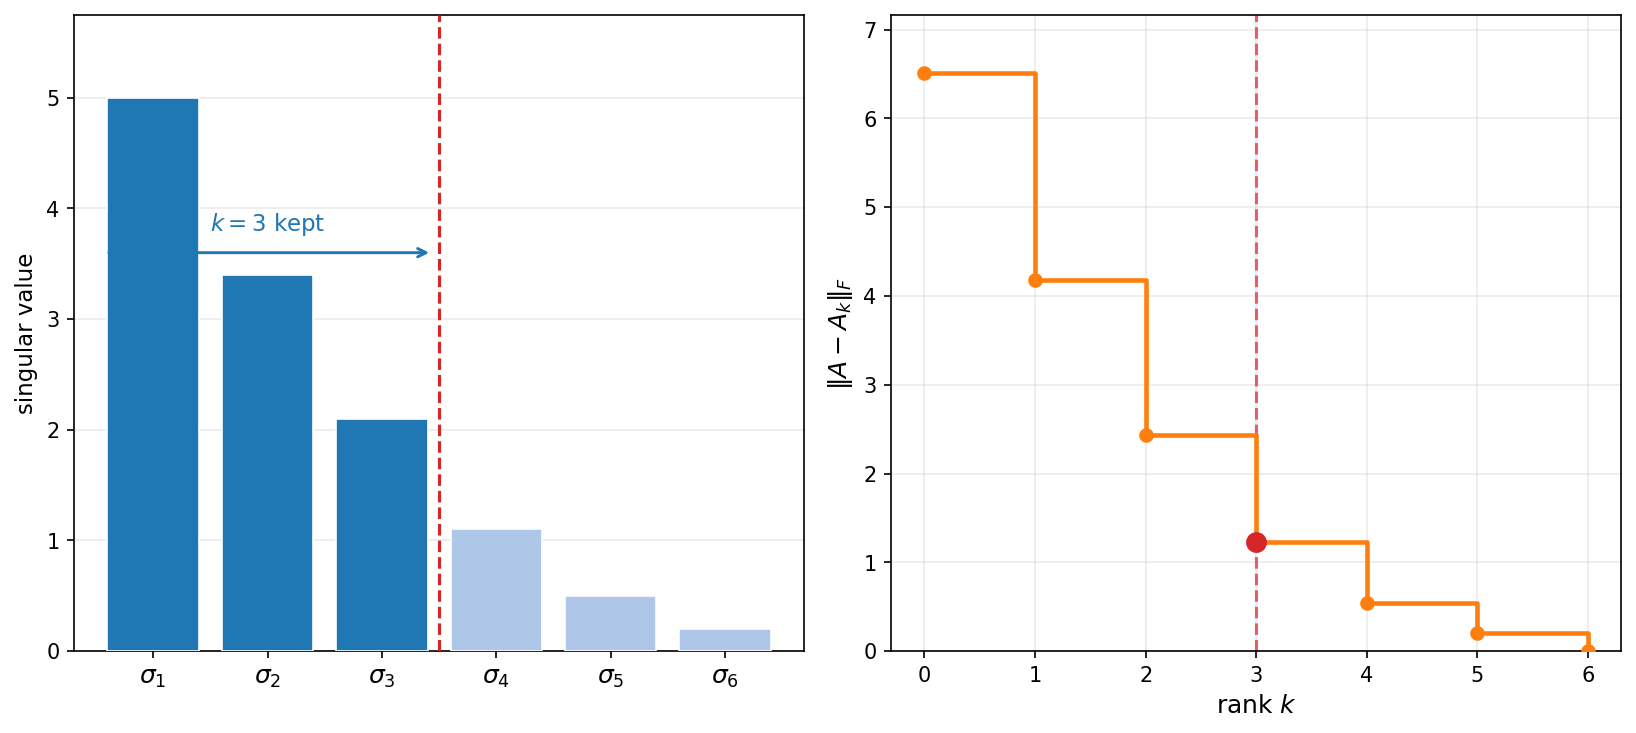
\includegraphics[width=\textwidth]{figures/fig10_eckart_young.png}
  \caption{Eckart--Young theorem illustrated on a $6\times 8$ matrix with
    prescribed singular value decay.
    \emph{Left:} singular value spectrum; blue bars ($\sigma_1,\sigma_2,\sigma_3$)
    are kept, light bars are discarded.
    \emph{Right:} Frobenius approximation error $\|A-A_k\|_F$ vs.\ rank $k$;
    the red dot marks $k=3$.
    Each step down corresponds to including one more singular value.}
\end{figure}

% ============================================================
\subsection*{Applications}
% ============================================================

\subsubsection*{1.\ Image compression}

A greyscale image is a matrix $A\in\mathbb{R}^{m\times n}$ of pixel intensities.
Storing all $mn$ entries is expensive.  The rank-$k$ approximation $A_k$
requires storing $U_k$ ($m\times k$), $\Sigma_k$ ($k$ values), and $V_k$
($n\times k$): a total of $k(m+n+1)$ numbers.

\medskip\noindent
\textbf{Compression ratio:} $\dfrac{mn}{k(m+n+1)} \approx \dfrac{\min(m,n)}{2k}$
for square images.  Breakeven (no saving) at $k \approx mn/(m+n)$.

\medskip\noindent
\textbf{Quality:} Eckart--Young guarantees the truncation error $\|A-A_k\|_F^2 =
\sum_{i>k}\sigma_i^2$.  For natural images, singular values decay rapidly, so
even $k\ll \min(m,n)$ captures most of the visual content.

\begin{lstlisting}
import numpy as np
import matplotlib.pyplot as plt

# Synthetic "image": sum of low-rank structures + noise
rng = np.random.default_rng(1)
m, n = 128, 128
# True signal: rank-5
U0 = np.linalg.qr(rng.standard_normal((m, 5)))[0]
V0 = np.linalg.qr(rng.standard_normal((n, 5)))[0]
s0 = np.array([100., 60., 30., 15., 5.])
A_true = U0 @ np.diag(s0) @ V0.T
A_noisy = A_true + 3 * rng.standard_normal((m, n))

U, s, Vt = np.linalg.svd(A_noisy, full_matrices=False)

fig, axes = plt.subplots(1, 4, figsize=(14, 3))
axes[0].imshow(A_true, cmap='gray'); axes[0].set_title('True (rank 5)')
for ax, k in zip(axes[1:], [2, 5, 20]):
    Ak = U[:, :k] @ np.diag(s[:k]) @ Vt[:k, :]
    ax.imshow(Ak, cmap='gray')
    err = np.linalg.norm(A_noisy - Ak, 'fro')
    storage_pct = 100 * k * (m + n + 1) / (m * n)
    ax.set_title(f'k={k}, {storage_pct:.1f}% storage\nerr={err:.1f}')
plt.tight_layout(); plt.show()

# Singular value decay
plt.figure(figsize=(5, 3))
plt.semilogy(s[:30], 'o-')
plt.axvline(5, color='r', linestyle='--', label='true rank')
plt.xlabel('index $i$'); plt.ylabel('$\\sigma_i$')
plt.title('Singular value decay'); plt.legend(); plt.show()
\end{lstlisting}

% ------------------------------------------------------------------
\subsubsection*{2.\ Principal Component Analysis (PCA)}

\textbf{Setup.}  Given a data matrix $X\in\mathbb{R}^{N\times d}$ ($N$ samples,
$d$ features), first \emph{centre}: subtract the column means so each feature
has mean zero.  The (scaled) sample covariance is
\[
  C = \tfrac{1}{N}X^TX \in \mathbb{R}^{d\times d},
\]
which is PSD.  By the spectral theorem $C = V\Lambda V^T$ with $V$ orthogonal
and $\Lambda = \operatorname{diag}(\lambda_1,\ldots,\lambda_d)$, $\lambda_1\ge\cdots\ge 0$.

\medskip\noindent
\textbf{Connection to SVD.}  The SVD of $X/\sqrt{N} = U\Sigma V^T$ gives
$C = V\Sigma^2 V^T$, so the right singular vectors $v_i$ of $X$ \emph{are}
the eigenvectors of $C$.  The $i$-th \emph{principal component} is $v_i$
(direction of $i$-th most variance).  The variance along $v_i$ is $\sigma_i^2/N$.

\medskip\noindent
\textbf{Dimensionality reduction.}  Project the data onto the top $k$
components:
\[
  \tilde{X} = X V_k \in \mathbb{R}^{N\times k}, \quad
  V_k = [v_1\mid\cdots\mid v_k].
\]
Fraction of variance retained: $\sum_{i=1}^k \sigma_i^2 / \sum_i \sigma_i^2$.
Eckart--Young guarantees $\tilde{X}$ is the best rank-$k$ summary of $X$.

\begin{lstlisting}
import numpy as np
import matplotlib.pyplot as plt

rng = np.random.default_rng(2)

# 2D data: elongated cloud at 45 degrees
N = 300
t = rng.standard_normal(N)
X_raw = np.column_stack([3*t + 0.3*rng.standard_normal(N),
                         3*t + 0.3*rng.standard_normal(N)])
X = X_raw - X_raw.mean(axis=0)  # centre

# SVD of X
U, s, Vt = np.linalg.svd(X, full_matrices=False)
print("Singular values:", s.round(2))
print("Variance explained by PC1:", (s[0]**2 / np.sum(s**2) * 100).round(1), "%")

# First principal component = first row of Vt
pc1 = Vt[0]
print("PC1 direction:", pc1.round(3))   # approx [1/sqrt(2), 1/sqrt(2)]

# Projected (1D) data
X_proj = (X @ pc1[:, None]) * pc1[None, :]   # rank-1 reconstruction

plt.figure(figsize=(5, 4))
plt.scatter(X[:, 0], X[:, 1], alpha=0.3, s=10, label='data')
plt.plot(*X_proj.T, 'r.', markersize=3, label='projection onto PC1')
plt.quiver(0, 0, *pc1*6, angles='xy', scale_units='xy', scale=1,
           color='k', width=0.02, label='PC1')
plt.axis('equal'); plt.legend(); plt.title('PCA on elongated data'); plt.show()
\end{lstlisting}

\begin{figure}[h!]
  \centering
  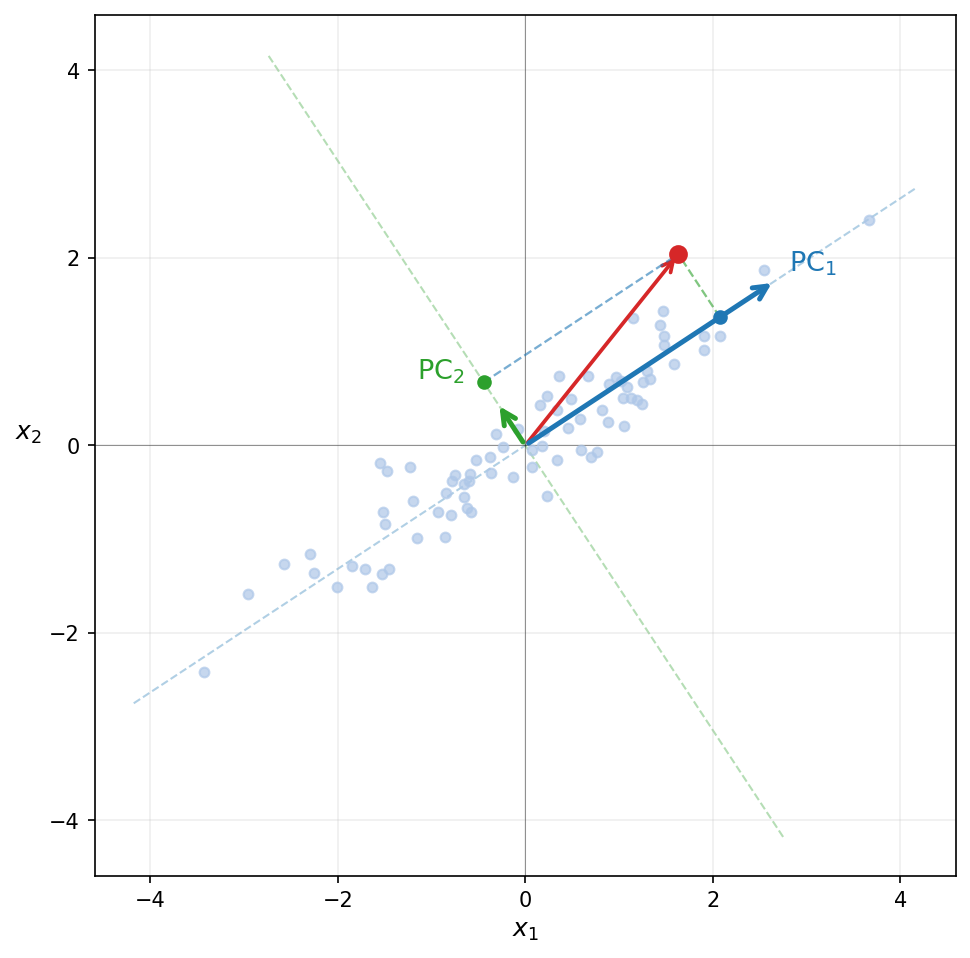
\includegraphics[width=0.72\textwidth]{figures/fig11_pca.png}
  \caption{PCA on a correlated 2D data cloud.
    $\mathrm{PC}_1$ (blue) points along the direction of maximum variance;
    $\mathrm{PC}_2$ (green) is orthogonal.
    Dashed lines extend each axis across the full plot.
    The red point decomposes as $x = z_1\,\mathrm{PC}_1 + z_2\,\mathrm{PC}_2$:
    the blue dot is its foot on the $\mathrm{PC}_1$ axis (score $z_1$),
    the green dot is its foot on the $\mathrm{PC}_2$ axis (score $z_2$).}
\end{figure}

% ------------------------------------------------------------------
% Sections 3 (Denoising) and 4 (LoRA) removed to lab exercises.
% See TODO.md for lab ideas.
\subsubsection*{Further applications (lab ideas)}

\begin{itemize}
  \item \textbf{Denoising.}  Model $M = A_{\text{signal}} + E$ (low-rank signal
        plus noise).  Compute the SVD of $M$ and look for an ``elbow'' in the
        singular value plot to pick the truncation rank $k$.
  \item \textbf{LoRA (Low-Rank Adaptation).}  In large language models, weight
        updates $\Delta W = AB^T$ are constrained to rank $r \ll \min(m,n)$,
        reducing trainable parameters from $mn$ to $r(m+n)$.  This is Eckart--Young
        applied to gradient updates.
\end{itemize}

\subsection*{Python: SVD basics and error formula}
\begin{lstlisting}
import numpy as np

rng = np.random.default_rng(0)

# ---- Verify A = U Sigma V^T ----
A = rng.standard_normal((4, 6))
U, s, Vt = np.linalg.svd(A, full_matrices=True)
Sigma = np.zeros_like(A, dtype=float)
np.fill_diagonal(Sigma, s)
print("A = U Sigma V^T:", np.allclose(A, U @ Sigma @ Vt))
print("U orthogonal:", np.allclose(U.T @ U, np.eye(U.shape[0])))
print("V orthogonal:", np.allclose(Vt @ Vt.T, np.eye(Vt.shape[0])))

# ---- Eckart-Young error formula ----
B = rng.standard_normal((5, 3))
M = B @ rng.standard_normal((3, 8)) + 0.2 * rng.standard_normal((5, 8))
U2, s2, Vt2 = np.linalg.svd(M, full_matrices=False)
print("\nSingular values:", s2.round(3))
for k in [1, 2, 3, 4]:
    Mk = U2[:, :k] @ np.diag(s2[:k]) @ Vt2[:k, :]
    err_frob   = np.linalg.norm(M - Mk, 'fro')
    err_formula = np.sqrt(np.sum(s2[k:]**2))
    print(f"k={k}: ||A-Ak||_F={err_frob:.4f}  formula={err_formula:.4f}  match={np.isclose(err_frob, err_formula)}")
\end{lstlisting}

% ============================================================
\section{Determinants (Geometric Approach)}
% ============================================================

\begin{definition}[Multilinear alternating form]
  For $A = [a_1\mid\cdots\mid a_n]$ with columns $a_i\in\mathbb{R}^n$, the
  \emph{determinant} is the unique function
  $\det:\mathbb{R}^{n\times n}\to\mathbb{R}$ such that:
  \begin{enumerate}
    \item $\det$ is \emph{multilinear} in the columns.
    \item $\det$ is \emph{alternating}: swapping two columns flips the sign;
          repeated columns give $0$.
    \item $\det(I) = 1$.
  \end{enumerate}
\end{definition}

\begin{remark}[Geometric meaning]
  $|\det(A)|$ is the \emph{volume-scaling factor} of the linear map
  $x\mapsto Ax$.  The sign records orientation.
  For $n=2$: $|\det(A)|$ is the area of the parallelogram spanned by the columns.
\end{remark}

\begin{figure}[h!]
  \centering
  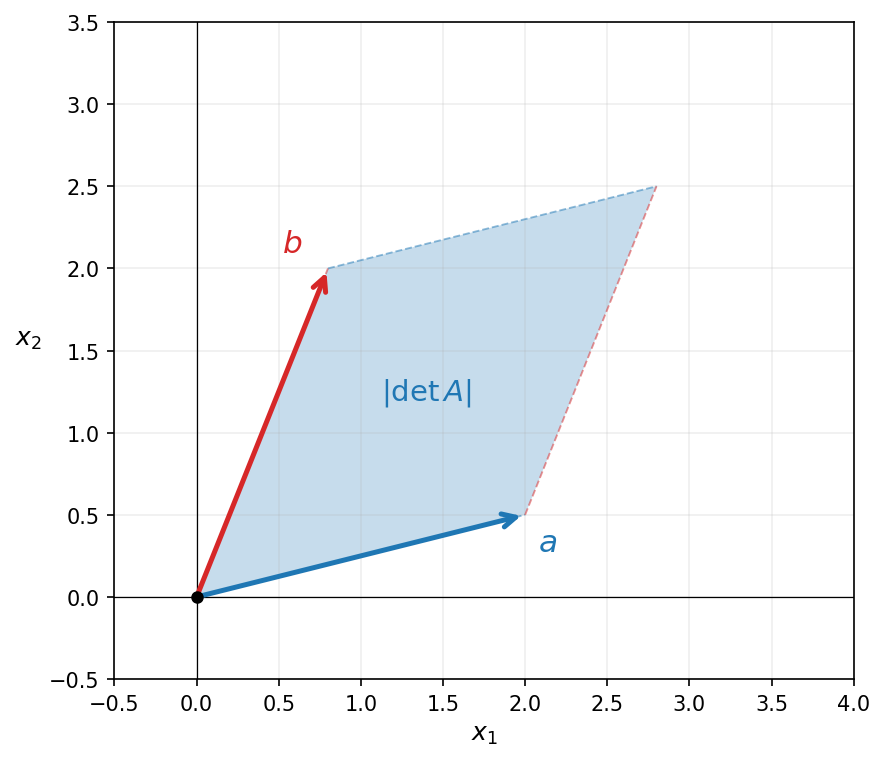
\includegraphics[width=0.55\textwidth]{figures/fig12_determinant.png}
  \caption{Determinant as area in $\mathbb{R}^2$.
    Vectors $a$ (blue) and $b$ (red) span the shaded parallelogram;
    its area equals $|\det[a\mid b]| = |a_1 b_2 - a_2 b_1|$.}
\end{figure}

\begin{proposition}
  $\det(A) = 0$ iff the columns of $A$ are linearly dependent.
\end{proposition}

\begin{proposition}[Multiplicativity]
  $\det(AB) = \det(A)\det(B)$.
\end{proposition}
\begin{proof}
  Both sides are multilinear alternating in the columns of $B$ and agree when
  $B = I$, so they are equal by uniqueness.
\end{proof}

\begin{remark}[Leibniz formula and cofactor expansion]
  The Leibniz formula:
  \[
    \det(A) = \sum_{\pi\in S_n}\operatorname{sgn}(\pi)\prod_{i=1}^n a_{i,\pi(i)}.
  \]
  Cofactor expansion along row $i$:
  \[
    \det(A) = \sum_{j=1}^n (-1)^{i+j} a_{ij}\det(M_{ij}),
  \]
  where $M_{ij}$ is the $(n-1)\times(n-1)$ minor obtained by deleting row $i$
  and column $j$.
\end{remark}

\subsection*{Python example}
\begin{lstlisting}
import numpy as np

A = np.array([[2, 1],
              [1, 3]], float)
print("det(A) =", np.linalg.det(A))  # = 5

# 2D area scaling
x = np.array([1.0, 0.0])
y = np.array([0.0, 1.0])
area_before = abs(np.linalg.det(np.column_stack([x, y])))
area_after  = abs(np.linalg.det(A @ np.column_stack([x, y])))
print("area before:", area_before, "  after:", area_after)
# area_after / area_before == |det(A)| == 5
\end{lstlisting}

% ----------------------------------------------------------------
\subsection*{The symmetric group $S_n$ and the sign of a permutation}
% ----------------------------------------------------------------

A \emph{permutation} of $\{1,\ldots,n\}$ is a bijection
$\pi:\{1,\ldots,n\}\to\{1,\ldots,n\}$.
The set of all $n!$ such bijections, together with composition as the group
operation, is the \emph{symmetric group} $S_n$.

\begin{definition}[Transposition]
  A \emph{transposition} is a permutation that swaps exactly two elements
  and fixes all others.  Every permutation can be written as a (non-unique)
  product of transpositions.
\end{definition}

\begin{definition}[Sign / signature]
  Although the decomposition into transpositions is not unique, the
  \emph{parity} of the number of transpositions is an invariant of $\pi$.
  The \emph{sign} (or \emph{signature}) of $\pi$ is
  \[
    \operatorname{sgn}(\pi)
    \;=\;
    \begin{cases}
      +1 & \text{if $\pi$ is a product of an \emph{even} number of transpositions,}\\
      -1 & \text{if $\pi$ is a product of an \emph{odd} number of transpositions.}
    \end{cases}
  \]
  Equivalently, $\operatorname{sgn}(\pi) = \prod_{i<j}\frac{\pi(j)-\pi(i)}{j-i}
  \in\{+1,-1\}$.
\end{definition}

\begin{remark}[Sign is a group homomorphism]
  $\operatorname{sgn}:S_n\to\{+1,-1\}$ is a group homomorphism:
  $\operatorname{sgn}(\pi\circ\sigma)=\operatorname{sgn}(\pi)\,\operatorname{sgn}(\sigma)$.
  The \emph{even} permutations (sign $+1$) form the \emph{alternating group}
  $A_n\trianglelefteq S_n$ of index~$2$ and order $n!/2$.
\end{remark}

\begin{example}[$S_3$]
  $S_3$ has $6$ elements.
  The identity $e$ and the two $3$-cycles $(123),(132)$ are even
  (sign $+1$); the three transpositions $(12),(13),(23)$ are odd
  (sign $-1$).
\end{example}

% ----------------------------------------------------------------
\subsection*{Uniqueness: the three axioms pin down $\det$}
% ----------------------------------------------------------------

The definition stated three axioms.  We now show they are enough to
determine $\det$ completely --- and derive the Leibniz formula as a
consequence.

\begin{proposition}[Uniqueness and Leibniz formula]
  The three axioms (multilinearity, alternating, normalisation
  $\det(I)=1$) determine $\det$ uniquely.  Every function satisfying
  them equals
  \[
    \det(A)
    = \sum_{\pi\in S_n}\operatorname{sgn}(\pi)\prod_{i=1}^n a_{i,\pi(i)},
  \]
  where $S_n$ is the set of all permutations of $\{1,\ldots,n\}$ and
  $\operatorname{sgn}(\pi)\in\{+1,-1\}$ is the \emph{signature} of $\pi$
  ($+1$ if $\pi$ is a product of an even number of transpositions,
  $-1$ otherwise).
\end{proposition}
\begin{proof}
  Write each column in the standard basis:
  $a_j = \sum_{i=1}^n a_{ij}e_i$.
  Expand $\det(a_1,\ldots,a_n)$ by multilinearity in every column
  simultaneously:
  \[
    \det(A)
    = \sum_{i_1=1}^n\cdots\sum_{i_n=1}^n
      a_{i_1 1}\,a_{i_2 2}\cdots a_{i_n n}
      \;\det(e_{i_1},e_{i_2},\ldots,e_{i_n}).
  \]
  There are $n^n$ terms.  By the alternating axiom,
  $\det(e_{i_1},\ldots,e_{i_n})=0$ whenever any two indices coincide.
  Only the $n!$ terms in which $(i_1,\ldots,i_n)$ is a permutation
  $\pi$ of $\{1,\ldots,n\}$ survive.

  For any permutation $\pi$, decompose it into transpositions.
  Each transposition swaps two columns and flips the sign once, so
  \[
    \det(e_{\pi(1)},\ldots,e_{\pi(n)})
    = \operatorname{sgn}(\pi)\,\det(e_1,\ldots,e_n)
    = \operatorname{sgn}(\pi)\cdot 1.
  \]
  Collecting all surviving terms:
  \[
    \det(A) = \sum_{\pi\in S_n}\operatorname{sgn}(\pi)
              \prod_{i=1}^n a_{i,\pi(i)}.
  \]
  This formula is forced by the axioms; there is no freedom left.
  Hence $\det$ is unique.
\end{proof}

\begin{example}[$n=2$]
  $S_2 = \{\mathrm{id}, (12)\}$ with signatures $+1,-1$:
  \[
    \det\begin{pmatrix}a&b\\c&d\end{pmatrix}
    = (+1)\cdot a\cdot d + (-1)\cdot b\cdot c = ad-bc.
  \]
\end{example}

% ----------------------------------------------------------------
\subsection*{Computing $\det$ via column reduction}
% ----------------------------------------------------------------

The same column operations from \S1.6 (which preserved $\operatorname{im}A$)
have a precise and simple effect on $\det$.

\begin{proposition}[Effect of column operations on $\det$]
  \leavevmode
  \begin{enumerate}
    \item \textbf{Add a multiple:}
          $\bar a_j \leftarrow \bar a_j + \lambda\bar a_i$, $i\ne j$:
          \quad $\det$ is \emph{unchanged}.
    \item \textbf{Scale a column:}
          $\bar a_j \leftarrow \lambda\bar a_j$:\quad $\det$ is
          \emph{multiplied by $\lambda$}.
    \item \textbf{Swap:}
          $\bar a_i \leftrightarrow \bar a_j$:\quad $\det$
          \emph{changes sign}.
  \end{enumerate}
\end{proposition}
\begin{proof}
  (1) By multilinearity in column $j$:
  \[
    \det(\ldots,\,a_j+\lambda a_i,\,\ldots)
    = \det(\ldots,a_j,\ldots)
    + \lambda\det(\ldots,a_i,\ldots,a_i,\ldots).
  \]
  The second term has column $i$ repeated, so it vanishes by the
  alternating axiom.

  (2) Multilinearity in column $j$:
  $\det(\ldots,\lambda a_j,\ldots)=\lambda\det(\ldots,a_j,\ldots)$.

  (3) Direct consequence of the alternating axiom.
\end{proof}

\begin{remark}[Algorithm for $\det$]
  Column-reduce $A$ to upper-triangular $T$ using the operations above.
  Track all scalings $\lambda_1,\ldots,\lambda_s$ and the number of
  swaps $k$.  Then
  \[
    \det(A)
    = (-1)^k \cdot
      \frac{1}{\lambda_1\cdots\lambda_s}
      \cdot \prod_{i=1}^n t_{ii}.
  \]
  A zero pivot appears iff the columns are linearly dependent, giving
  $\det(A)=0$.  This is what \texttt{np.linalg.det} computes internally
  (via LU factorisation with partial pivoting).
\end{remark}

\begin{proposition}
  $\det(A^T) = \det(A)$.
\end{proposition}
\begin{proof}
  In the Leibniz formula, $(A^T)_{i,\pi(i)} = a_{\pi(i),i}$.
  Substitute $\sigma = \pi^{-1}$; as $\pi$ ranges over $S_n$, so does
  $\sigma$, and $\operatorname{sgn}(\pi^{-1})=\operatorname{sgn}(\pi)$.
  Setting $j=\pi(i)$ (equivalently $i=\sigma(j)$):
  \[
    \prod_{i=1}^n a_{\pi(i),i}
    = \prod_{j=1}^n a_{j,\sigma(j)}.
  \]
  Hence $\det(A^T)
  = \sum_\sigma \operatorname{sgn}(\sigma)\prod_j a_{j,\sigma(j)}
  = \det(A)$.
\end{proof}

\begin{remark}
  Transposing interchanges rows and columns, so $\det(A^T)=\det(A)$
  means the alternating property holds equally in the rows.  All results
  stated for columns have row analogues.
\end{remark}

\begin{proposition}[$|\det A| = $ product of singular values]
\label{prop:det-svd}
  For $A\in\mathbb{R}^{n\times n}$ with singular values
  $\sigma_1\ge\cdots\ge\sigma_n\ge 0$:
  \[
    |\det(A)| = \sigma_1\sigma_2\cdots\sigma_n.
  \]
\end{proposition}
\begin{proof}
  Write $A = U\Sigma V^T$ (SVD, Thm.~\ref{thm:svd}).
  By multiplicativity of $\det$:
  \[
    \det(A) = \det(U)\cdot\det(\Sigma)\cdot\det(V^T).
  \]
  Since $U^TU = I$, taking $\det$ gives $\det(U)^2=1$, so
  $\det(U)\in\{+1,-1\}$.  Likewise $\det(V^T)\in\{+1,-1\}$.
  Thus
  \[
    |\det(A)| = |\det(\Sigma)| = \prod_{i=1}^n\sigma_i.
  \]
\end{proof}

\begin{corollary}
  $\det(A)=0$ iff $A$ is singular iff some $\sigma_i=0$
  iff $\operatorname{rank}(A)<n$.
  This connects the determinant criterion for invertibility to the
  kernel/image criterion of \S1.6 and the spectral criterion of \S4.2.
\end{corollary}

\subsection*{Python: determinants in practice}
\begin{lstlisting}
import numpy as np
from itertools import permutations

def leibniz_det(A):
    """Compute det(A) via the Leibniz formula (slow, illustrative)."""
    n = A.shape[0]
    total = 0.0
    for pi in permutations(range(n)):
        inv = sum(1 for i in range(n) for j in range(i+1, n) if pi[i] > pi[j])
        sign = (-1) ** inv
        prod = 1.0
        for i in range(n):
            prod *= A[i, pi[i]]
        total += sign * prod
    return total

A = np.array([[2., 1., 0.],
              [1., 3., 1.],
              [0., 1., 2.]])

print("Leibniz:     ", round(leibniz_det(A), 10))   # 8.0
print("np.linalg:   ", round(np.linalg.det(A), 10)) # 8.0

# |det| = product of singular values
s = np.linalg.svd(A, compute_uv=False)
print("prod sigma_i:", round(np.prod(s), 10))        # 8.0

# Column operations tracking det
B = A.copy()
B[:, 0] *= 2        # scale col 0 by 2: det(B) = 2 * det(A) = 16
print("After scaling col 0:", round(np.linalg.det(B), 10))   # 16.0

C = A[:, [1, 0, 2]] # swap columns 0 and 1: det changes sign
print("After swap col 0<->1:", round(np.linalg.det(C), 10))  # -8.0
\end{lstlisting}


% ================================================================
% NEW SECTION: Tensor Products
% ================================================================

\section{Tensor Products}

\subsection*{Motivation: bilinear maps}

Linear maps take one vector input and are linear in it.  Many natural
operations in the course take \emph{two} vector inputs and are linear in
each:
\begin{itemize}
  \item The inner product $\langle u,v\rangle: V\times V\to\mathbb{R}$
        (bilinear, symmetric --- \S3).
  \item Matrix multiplication $(A,B)\mapsto AB:
        \mathbb{R}^{m\times n}\times\mathbb{R}^{n\times p}
        \to\mathbb{R}^{m\times p}$ (bilinear).
  \item The outer product $(u,v)\mapsto uv^T:
        \mathbb{R}^m\times\mathbb{R}^n\to\mathbb{R}^{m\times n}$
        (bilinear; appears in the SVD outer-product expansion).
\end{itemize}

\begin{definition}[Bilinear map]
  A map $T: V\times W \to Z$ is \emph{bilinear} if it is linear in each
  argument with the other held fixed:
  \[
    T(\lambda u + \mu v,\, w) = \lambda T(u,w)+\mu T(v,w), \quad
    T(v,\, \lambda u + \mu w) = \lambda T(v,u)+\mu T(v,w).
  \]
  More generally, $T: V_1\times\cdots\times V_k\to Z$ is
  \emph{$k$-multilinear} if it is linear in each argument separately.
\end{definition}

\begin{remark}
  A bilinear map is \emph{not} a linear map from $V\times W$: linearity
  would require $T(u+v, w+x) = T(u,w)+T(u,x)+T(v,w)+T(v,x)$, but the
  bilinear condition only gives $T(u+v,w) = T(u,w)+T(v,w)$ (one slot
  at a time).  The difference is the mixed/crossed terms.
\end{remark}

% ----------------------------------------------------------------
\subsection*{The tensor product $V\otimes W$}
% ----------------------------------------------------------------

The tensor product packages the data of all bilinear maps into a single
linear-algebra object.

\begin{definition}[Tensor product of vector spaces]
  Let $V=\mathbb{R}^m$ with standard basis $\{e_1,\ldots,e_m\}$ and
  $W=\mathbb{R}^n$ with standard basis $\{f_1,\ldots,f_n\}$.
  The \emph{tensor product} $V\otimes W$ is the vector space of dimension
  $mn$ with basis
  \[
    \bigl\{e_i\otimes f_j : 1\le i\le m,\; 1\le j\le n\bigr\}.
  \]
  For $v=\sum_i v_i e_i\in V$ and $w=\sum_j w_j f_j\in W$, define
  \[
    v\otimes w
    \;=\; \sum_{i,j} v_i w_j\,(e_i\otimes f_j)
    \;\in\; V\otimes W.
  \]
\end{definition}

\begin{remark}[Tensor product = outer product, concretely]
  The coefficient array of $v\otimes w$ is $(v_i w_j)$, which is exactly
  the \emph{outer product matrix} $vw^T\in\mathbb{R}^{m\times n}$.
  So $V\otimes W \cong \mathbb{R}^{m\times n}$ as a vector space, with
  simple tensors corresponding to rank-1 matrices.
\end{remark}

\begin{remark}[Not every tensor is a simple tensor]
  The element $e_1\otimes f_1 + e_2\otimes f_2\in V\otimes W$ corresponds
  to the matrix $\begin{pmatrix}1&0\\0&1\end{pmatrix}$, which has rank 2
  and cannot be written as a single $vw^T$.  The general element of
  $V\otimes W$ is $\sum_{i,j}t_{ij}(e_i\otimes f_j)$, corresponding to an
  arbitrary matrix $T\in\mathbb{R}^{m\times n}$.

  The \emph{tensor rank} of $T$ is the minimum number of simple tensors
  needed; this equals the matrix rank.  The SVD outer-product expansion
  $A = \sum_{k=1}^r \sigma_k u_k v_k^T$ is a decomposition of $A$ into
  $r$ simple tensors --- the minimum possible by Eckart--Young.
\end{remark}

\begin{proposition}[Universal property]
  Every bilinear map $T: V\times W\to Z$ factors uniquely through
  $V\otimes W$: there is a unique linear map $\tilde T: V\otimes W\to Z$
  such that $T(v,w) = \tilde T(v\otimes w)$ for all $v,w$.

  Conversely, specifying a linear map on $V\otimes W$ is equivalent to
  specifying a bilinear map on $V\times W$.
\end{proposition}
\begin{proof}[Proof sketch]
  Define $\tilde T$ on basis elements by
  $\tilde T(e_i\otimes f_j) = T(e_i,f_j)$ and extend by linearity.
  This is well-defined and unique.  Bilinearity of $T$ ensures
  $\tilde T(v\otimes w) = T(v,w)$ for all simple tensors, hence
  for all $V\times W$.
\end{proof}

\begin{remark}
  The universal property says: \emph{bilinear is the same as linear once
  you pass through $\otimes$}.  It is the same move made in \S1.5:
  every linear map $V\to W$ is determined by what it does to a basis.
  Here: every bilinear map $V\times W\to Z$ is determined by what it
  does to basis pairs $(e_i,f_j)$, which becomes a linear map on
  $V\otimes W$.
\end{remark}

% ----------------------------------------------------------------
\subsection*{The Kronecker product}
% ----------------------------------------------------------------

If $A: V\to V'$ and $B: W\to W'$ are linear maps, the map
$(v,w)\mapsto (Av)\otimes(Bw)$ is bilinear from $V\times W$ into
$V'\otimes W'$.  By the universal property it factors through a linear
map $A\otimes B: V\otimes W\to V'\otimes W'$.

\begin{definition}[Kronecker product]
  For $A\in\mathbb{R}^{m\times n}$ and $B\in\mathbb{R}^{p\times q}$, the
  \emph{Kronecker product} $A\otimes B\in\mathbb{R}^{mp\times nq}$ is the
  block matrix
  \[
    A\otimes B
    = \begin{pmatrix}
        a_{11}B & a_{12}B & \cdots & a_{1n}B \\
        a_{21}B & a_{22}B & \cdots & a_{2n}B \\
        \vdots  &         & \ddots & \vdots  \\
        a_{m1}B & a_{m2}B & \cdots & a_{mn}B
      \end{pmatrix}.
  \]
  It acts on simple tensors by $(A\otimes B)(v\otimes w) = (Av)\otimes(Bw)$.
\end{definition}

\begin{proposition}[Mixed-product property]
  $(A\otimes B)(C\otimes D) = (AC)\otimes(BD)$, whenever the dimensions
  are compatible.
\end{proposition}
\begin{proof}
  On simple tensors:
  $(A\otimes B)(C\otimes D)(v\otimes w)
  = (A\otimes B)((Cv)\otimes(Dw))
  = (ACv)\otimes(BDw)
  = (AC\otimes BD)(v\otimes w)$.
  Since simple tensors span, equality holds everywhere.
\end{proof}

\begin{corollary}[Eigenvalues of $A\otimes B$]
  If $Av = \lambda v$ and $Bw = \mu w$, then
  $(A\otimes B)(v\otimes w) = \lambda\mu\,(v\otimes w)$.
  In particular, if $A\in\mathbb{R}^{m\times m}$ has eigenvalues
  $\lambda_1,\ldots,\lambda_m$ and $B\in\mathbb{R}^{n\times n}$ has
  eigenvalues $\mu_1,\ldots,\mu_n$, then $A\otimes B$ has eigenvalues
  $\{\lambda_i\mu_j\}$.
\end{corollary}
\begin{proof}
  Immediate from the mixed-product property applied to $v\otimes w$.
\end{proof}

\begin{example}[Solving $AX + XB^T = C$]
  The \emph{Sylvester equation} $AX + XB^T = C$ arises in control theory
  and numerical linear algebra.  Applying $\operatorname{vec}$ (stack
  columns of $X$) and using
  $(I_n\otimes A)\operatorname{vec}(X) = \operatorname{vec}(AX)$ and
  $(B\otimes I_m)\operatorname{vec}(X) = \operatorname{vec}(XB^T)$:
  \[
    (I_n\otimes A + B\otimes I_m)\,\operatorname{vec}(X)
    = \operatorname{vec}(C).
  \]
  This is a standard $mn\times mn$ linear system.  It has a unique solution
  iff $A$ and $-B$ share no eigenvalue --- which, by the eigenvalue formula
  above, means $\lambda_i + \mu_j \ne 0$ for all $i,j$.
\end{example}

\subsection*{Python: Kronecker products}
\begin{lstlisting}
import numpy as np

A = np.array([[1., 2.],
              [3., 4.]])
B = np.array([[0., 5.],
              [6., 7.]])

K = np.kron(A, B)
print("A kron B:\n", K)
print("shape:", K.shape)   # (4, 4)

# Simple tensor = rank-1 matrix = outer product
v = np.array([1., 2., 3.])
w = np.array([4., 5.])
T = np.outer(v, w)         # v tensor w
print("\nv outer w:\n", T)
print("rank:", np.linalg.matrix_rank(T))  # 1

# Mixed-product: (A kron B)(u kron w) == (Au) kron (Bw)
A2 = np.array([[1., 0.], [0., -1.]])
B2 = np.array([[2., 1.], [0., 2.]])
u = np.array([1., 2.])
w2 = np.array([3., 4.])
lhs = np.kron(A2, B2) @ np.kron(u, w2)
rhs = np.kron(A2 @ u, B2 @ w2)
print("\nMixed-product check:", np.allclose(lhs, rhs))  # True

# Eigenvalues of A kron B = products of eigenvalues
lam_A = np.linalg.eigvals(A)
lam_B = np.linalg.eigvals(B)
expected = np.sort([a * b for a in lam_A for b in lam_B]).real
actual   = np.sort(np.linalg.eigvals(K)).real
print("Kronecker eigenvalues match:", np.allclose(expected, actual))
\end{lstlisting}


% ================================================================
% NEW SECTION: Alternating Forms and the Exterior Algebra
% ================================================================

\section{Alternating Forms and the Exterior Algebra}

\subsection*{From bilinear to alternating}

The determinant is the canonical example of an $n$-linear \emph{alternating}
form.  This section develops the full family of alternating forms, of which
$\det$ is the top member.

\begin{definition}[$k$-linear alternating form]
  A map $\omega: (\mathbb{R}^n)^k \to \mathbb{R}$ is a
  \emph{$k$-linear alternating form} (or \emph{$k$-form}) if:
  \begin{enumerate}
    \item It is linear in each of the $k$ arguments.
    \item $\omega(\ldots,v_i,\ldots,v_j,\ldots) =
          -\omega(\ldots,v_j,\ldots,v_i,\ldots)$
          whenever two arguments are swapped.
  \end{enumerate}
  Equivalently, $\omega(\ldots,v,\ldots,v,\ldots) = 0$ whenever two
  arguments coincide.  Write $\operatorname{Alt}^k(\mathbb{R}^n)$ for
  the space of all $k$-forms on $\mathbb{R}^n$.
\end{definition}

\begin{remark}[Alternating $\Leftrightarrow$ sign of $S_k$ acts]
  The alternating condition is equivalent to saying $\omega$ transforms
  under the sign representation of the symmetric group $S_k$: for any
  permutation $\pi\in S_k$,
  \[
    \omega(v_{\pi(1)},\ldots,v_{\pi(k)})
    = \operatorname{sgn}(\pi)\,\omega(v_1,\ldots,v_k).
  \]
  Each transposition contributes one sign flip, and since
  $\operatorname{sgn}$ is a homomorphism the total sign is
  $\operatorname{sgn}(\pi)$ regardless of how $\pi$ is factored.
  This is precisely why the Leibniz formula for $\det$ sums over $S_n$
  with weights $\operatorname{sgn}(\pi)$.
\end{remark}

\begin{example}
  \leavevmode
  \begin{itemize}
    \item $\operatorname{Alt}^0(\mathbb{R}^n) = \mathbb{R}$ (constants).
    \item $\operatorname{Alt}^1(\mathbb{R}^n)$: linear functionals
          $\mathbb{R}^n\to\mathbb{R}$ (the dual space).
    \item $\operatorname{Alt}^2(\mathbb{R}^2)$: every 2-form satisfies
          $\omega(u,v) = c(u_1v_2-u_2v_1)$ for some $c\in\mathbb{R}$.
          For $c=1$ this is the signed area of the parallelogram spanned
          by $u$ and $v$.
    \item $\operatorname{Alt}^n(\mathbb{R}^n)$: 1-dimensional, spanned by
          $\det$ (proved in the uniqueness theorem above).
    \item $\operatorname{Alt}^k(\mathbb{R}^n)$ for $k>n$: must be $\{0\}$,
          since any $k>n$ vectors in $\mathbb{R}^n$ are linearly dependent
          and the alternating property forces $\omega=0$.
  \end{itemize}
\end{example}

\begin{proposition}[$\dim\operatorname{Alt}^k(\mathbb{R}^n) = \binom{n}{k}$]
\label{prop:dim-alt}
  A basis for $\operatorname{Alt}^k(\mathbb{R}^n)$ is indexed by
  $k$-element subsets $I = \{i_1 < \cdots < i_k\}\subset\{1,\ldots,n\}$:
  define $\omega_I$ by
  \[
    \omega_I(v_1,\ldots,v_k)
    = \det\bigl([v_1\mid\cdots\mid v_k]_I\bigr),
  \]
  where $[\cdot]_I$ is the $k\times k$ submatrix using rows $I$.
  These $\binom{n}{k}$ forms are linearly independent and span
  $\operatorname{Alt}^k(\mathbb{R}^n)$.
\end{proposition}
\begin{proof}[Proof sketch]
  Each $\omega_I$ is $k$-linear and alternating (inherited from $\det$).
  For any $k$-form $\omega$, its values on all $k$-tuples are determined
  by $\omega(e_{i_1},\ldots,e_{i_k})$ for $i_1<\cdots<i_k$ (by
  multilinearity and alternating, exactly as in the Leibniz proof).
  There are $\binom{n}{k}$ such values, giving $\dim\le\binom{n}{k}$.
  Linear independence of the $\omega_I$ gives equality.
\end{proof}

\begin{remark}[The dimension table]
  \begin{center}
  \renewcommand{\arraystretch}{1.3}
  \begin{tabular}{c|cccccc}
    $k$ & $0$ & $1$ & $2$ & $\cdots$ & $n-1$ & $n$ \\\hline
    $\dim$ & $1$ & $n$ & $\binom{n}{2}$ & $\cdots$ & $n$ & $1$
  \end{tabular}
  \end{center}
  The table is symmetric: $\binom{n}{k}=\binom{n}{n-k}$.  The top entry
  ($k=n$, dimension 1) is why $\det$ is unique up to normalisation.
\end{remark}

% ----------------------------------------------------------------
\subsection*{The wedge product}
% ----------------------------------------------------------------

\begin{definition}[Wedge product of 1-forms]
  For linear functionals $\alpha,\beta\in(\mathbb{R}^n)^*$ (1-forms),
  their \emph{wedge product} $\alpha\wedge\beta$ is the 2-form
  \[
    (\alpha\wedge\beta)(u,v)
    = \alpha(u)\beta(v) - \alpha(v)\beta(u).
  \]
  More generally, for $\omega\in\operatorname{Alt}^j$ and
  $\eta\in\operatorname{Alt}^k$:
  \[
    (\omega\wedge\eta)(v_1,\ldots,v_{j+k})
    = \frac{1}{j!\,k!}
      \sum_{\pi\in S_{j+k}}\operatorname{sgn}(\pi)\,
      \omega(v_{\pi(1)},\ldots,v_{\pi(j)})\,
      \eta(v_{\pi(j+1)},\ldots,v_{\pi(j+k)}).
  \]
\end{definition}

\begin{example}[Basis 2-forms via wedge]
  Let $e_i^*$ denote the $i$-th coordinate functional:
  $e_i^*(v) = v_i$.  Then
  \[
    (e_i^*\wedge e_j^*)(u,v)
    = u_iv_j - u_jv_i
    = \det\begin{pmatrix}u_i & v_i \\ u_j & v_j\end{pmatrix}
    = \omega_{\{i,j\}}(u,v).
  \]
  So $\{e_i^*\wedge e_j^* : i<j\}$ is exactly the basis from
  Prop.~\ref{prop:dim-alt}.
\end{example}

\begin{proposition}[Properties of $\wedge$]
  \leavevmode
  \begin{enumerate}
    \item \textbf{Associativity:}
          $(\omega\wedge\eta)\wedge\zeta = \omega\wedge(\eta\wedge\zeta)$.
    \item \textbf{Anti-commutativity:}
          $\omega\wedge\eta = (-1)^{jk}\,\eta\wedge\omega$
          for $\omega\in\operatorname{Alt}^j$, $\eta\in\operatorname{Alt}^k$.
    \item \textbf{Top form is the determinant:}
          \[
            e_1^*\wedge e_2^*\wedge\cdots\wedge e_n^* = \det.
          \]
  \end{enumerate}
\end{proposition}
\begin{proof}[Proof of (3)]
  By the definition of $\wedge$ applied $n-1$ times:
  $(e_1^*\wedge\cdots\wedge e_n^*)(v_1,\ldots,v_n)
  = \sum_\pi \operatorname{sgn}(\pi)\prod_i e_i^*(v_{\pi(i)})
  = \sum_\pi \operatorname{sgn}(\pi)\prod_i (v_{\pi(i)})_i$.
  Re-indexing with $\sigma=\pi^{-1}$:
  $= \sum_\sigma \operatorname{sgn}(\sigma)\prod_i (v_i)_{\sigma(i)}
  = \det([v_1\mid\cdots\mid v_n])$.
\end{proof}

% ----------------------------------------------------------------
\subsection*{The determinant as a map on alternating forms}
% ----------------------------------------------------------------

A linear map $A:\mathbb{R}^n\to\mathbb{R}^n$ acts on $k$-forms by
\emph{pullback}: for $\omega\in\operatorname{Alt}^k(\mathbb{R}^n)$,
\[
  (A^*\omega)(v_1,\ldots,v_k) = \omega(Av_1,\ldots,Av_k).
\]
This is again a $k$-form, so $A^*$ maps
$\operatorname{Alt}^k\to\operatorname{Alt}^k$.

For $k=n$: since $\operatorname{Alt}^n(\mathbb{R}^n)$ is 1-dimensional
(spanned by $\det$), the map $A^*$ must be multiplication by some
scalar $c(A)$:
\[
  (A^*\det)(v_1,\ldots,v_n)
  = \det(Av_1,\ldots,Av_n)
  = c(A)\,\det(v_1,\ldots,v_n).
\]
Evaluating at $(e_1,\ldots,e_n)$ gives $c(A) = \det(A)$.

\begin{theorem}[$\det(AB) = \det(A)\det(B)$ via pullback]
  Pullback is functorial: $(AB)^* = B^*\circ A^*$.  Therefore
  \[
    \det(AB)\cdot\det = (AB)^*\det = B^*(A^*\det)
    = B^*(\det(A)\cdot\det) = \det(A)\cdot B^*\det
    = \det(A)\det(B)\cdot\det.
  \]
  Evaluating at $(e_1,\ldots,e_n)$: $\det(AB) = \det(A)\det(B)$.
\end{theorem}

\begin{remark}
  This proof works because $\operatorname{Alt}^n$ is 1-dimensional:
  the multiplicativity of $\det$ is a consequence of there being
  \emph{no room} for any other behaviour.  The Leibniz-formula proof of
  multiplicativity used the same idea implicitly; the pullback argument
  makes the structure explicit.
\end{remark}

\subsection*{Python: alternating forms and volume}
\begin{lstlisting}
import numpy as np

def wedge_2form(i, j, u, v):
    """(e_i* wedge e_j*)(u, v) = u[i]*v[j] - u[j]*v[i]"""
    return u[i]*v[j] - u[j]*v[i]

# In R^3: the three basis 2-forms
u = np.array([1., 2., 3.])
v = np.array([4., 5., 6.])
w12 = wedge_2form(0, 1, u, v)  # = 1*5 - 4*2 = -3
w13 = wedge_2form(0, 2, u, v)  # = 1*6 - 4*3 = -6
w23 = wedge_2form(1, 2, u, v)  # = 2*6 - 5*3 = -3
print("omega_{01}(u,v) =", w12)
print("omega_{02}(u,v) =", w13)
print("omega_{12}(u,v) =", w23)

# These are the components of -(u x v)
print("u x v =", np.cross(u, v))   # [-3, 6, -3]

# Top form: det([u,v,w]) = (e0*^e1*^e2*)(u,v,w)
w = np.array([7., 8., 10.])
A = np.column_stack([u, v, w])
print("\ndet([u,v,w]) =", round(np.linalg.det(A), 10))

# Pullback: det(Av_1,...,Av_n) = det(A) * det(v_1,...,v_n)
rng = np.random.default_rng(0)
M  = rng.standard_normal((4, 4))
V  = rng.standard_normal((4, 4))
lhs = np.linalg.det(M @ V)
rhs = np.linalg.det(M) * np.linalg.det(V)
print("det(MV) = det(M)*det(V):", np.isclose(lhs, rhs))  # True
\end{lstlisting}

\begin{exercise}
  \leavevmode
  \begin{enumerate}
    \item Show that $\omega(u,v) = u_1v_2 - u_2v_1$ on $\mathbb{R}^2$
          satisfies $\omega(Au,Av) = \det(A)\,\omega(u,v)$ for every
          $A\in\mathbb{R}^{2\times 2}$.  Conclude: \emph{area scales
          by $|\det(A)|$}.
    \item In $\mathbb{R}^3$, the three components of $u\times v$ are
          $(u_2v_3-u_3v_2,\; u_3v_1-u_1v_3,\; u_1v_2-u_2v_1)$.
          Express each as a basis 2-form $\omega_I(u,v)$.
          Conclude that $u\times v$ encodes all of
          $\operatorname{Alt}^2(\mathbb{R}^3)$.
  \end{enumerate}
\end{exercise}

\end{document}
